\documentclass[oneside,numbers,spanish]{ezthesis}
\usepackage[T1]{fontenc}
\usepackage[utf8]{inputenc}
\usepackage{lmodern}
\usepackage[spanish,activeacute]{babel}
\usepackage{url}
\usepackage{upquote}
\usepackage{verbatim}
\usepackage{color}
\usepackage{listings}
\usepackage{caption}
\usepackage{xcolor}
\usepackage{graphicx} % Inserccion de imagenes.
\usepackage{caption}
\usepackage{longtable}
\usepackage[refpages]{gloss} % glosario


%colores
\definecolor{gray97}{gray}{.97}
\definecolor{gray45}{gray}{.45}
\definecolor{gray75}{gray}{.75}
\definecolor{bluekeywords}{rgb}{0.13,0.13,1}
\definecolor{greencomments}{rgb}{0,0.5,0}
\definecolor{redstrings}{rgb}{0.9,0,0}

\DeclareCaptionFont{white}{\color{white}}
\DeclareCaptionFormat{listing}{\colorbox{gray}{\parbox{\textwidth}{#1#2#3}}}
\captionsetup[lstlisting]{format=listing,labelfont=white,textfont=white}


%Configuración para el lenguaje c
\lstset{language= C,
showspaces=false,
showtabs=false,
breaklines=true,
showstringspaces=false,
breakatwhitespace=true,
escapeinside={(*@}{@*)},
commentstyle=\color{greencomments},
keywordstyle=\color{bluekeywords}\bfseries,
stringstyle=\color{redstrings},
basicstyle=\ttfamily,
backgroundcolor=\color{gray97},
%%%
numberstyle=\footnotesize,
numbers=left,
stepnumber=1,
numbersep=10pt,
tabsize=2,
breaklines=true,
prebreak = \raisebox{0ex}[0ex][0ex]{\ensuremath{\hookleftarrow}},
breakatwhitespace=false,
aboveskip={1.5\baselineskip},
columns=fixed,
upquote=true,
extendedchars=true,
%frame=bottomline,
frame=lines,
%frame=Ltbr,
}

%Configuración para el lenguaje sh
\lstset{language= sh,
showspaces=false,
showtabs=false,
breaklines=true,
showstringspaces=false,
breakatwhitespace=true,
escapeinside={(*@}{@*)},
commentstyle=\color{greencomments},
keywordstyle=\color{bluekeywords}\bfseries,
stringstyle=\color{redstrings},
basicstyle=\ttfamily,
backgroundcolor=\color{gray97},
%%%
numberstyle=\footnotesize,
numbers=left,
stepnumber=1,
numbersep=10pt,
tabsize=2,
breaklines=true,
prebreak = \raisebox{0ex}[0ex][0ex]{\ensuremath{\hookleftarrow}},
breakatwhitespace=false,
aboveskip={1.5\baselineskip},
columns=fixed,
upquote=true,
extendedchars=true,
%frame=bottomline,
frame=lines,
%frame=Ltbr,
}

% minimizar fragmentado de listados
\lstnewenvironment{listing}[1][]
   {\lstset{#1}\pagebreak[0]}{\pagebreak[0]}
 


\author{Zetina Moya José Enrique - 206200773}
\title{Sistema de antivirus y antispam implementado en un FPGA}
\degree{Licenciatura en Ingeniería en Computación}
\supervisor{M. en C. Oscar Alvarado Nava}
\institution{Universidad Autónoma Metropolitana Unidad Azcapotzalco}
\faculty{División de Ciencias Básicas e Ingeniería}

\hyperlinking
\begin{document}


%% # Portada de la tesis #
%% Mirar el archivo "titlepage.tex" para los detalles.
%% ## Construye tu propia portada ##
%% 
%% Una portada se conforma por una secuencia de "Blocks" que incluyen
%% piezas individuales de informaci'on. Un "Block" puede incluir, por
%% ejemplo, el t'itulo del documento, una im'agen (logotipo de la universidad),
%% el nombre del autor, nombre del supervisor, u cualquier otra pieza de
%% informaci'on.
%%
%% Cada "Block" aparece centrado horizontalmente en la p'agina y,
%% verticalmente, todos los "Blocks" se distruyen de manera uniforme 
%% a lo largo de p'agina.
%%
%% Nota tambi'en que, dentro de un mismo "Block" se pueden cortar
%% lineas usando el comando \\
%%
%% El tama'no del texto dentro de un "Block" se puede modificar usando uno de
%% los comandos:
%%   \small      \LARGE
%%   \large      \huge
%%   \Large      \Huge
%%
%% Y el tipo de letra se puede modificar usando:
%%   \bfseries - negritas
%%   \itshape  - it'alicas
%%   \scshape  - small caps
%%   \slshape  - slanted
%%   \sffamily - sans serif
%%
%% Para producir plantillas generales, la informaci'on que ha sido inclu'ida
%% en el archivo principal "tesis.tex" se puede accesar aqu'i usando:
%%   \insertauthor
%%   \inserttitle
%%   \insertsupervisor
%%   \insertinstitution
%%   \insertdegree
%%   \insertfaculty
%%   \insertdepartment
%%   \insertsubmitdate

\begin{titlepage}
  \TitleBlock{\scshape\insertinstitution}
  \TitleBlock[\bigskip]{\scshape\insertfaculty}
  \TitleBlock{\Huge\scshape\inserttitle}
  \TitleBlock{\scshape
  \insertauthor \\
  \insertdegree \\
  Asesor \insertsupervisor }
  \TitleBlock{Octubre de \insertsubmitdate}
\end{titlepage}

%% Nota 1:
%% Se puede agregar un escudo o logotipo en un "Block" como:
%%   \TitleBlock{\includegraphics[height=4cm]{escudo_uni}}
%% y teniendo un archivo "escudo_uni.pdf", "escudo_uni.png" o "escudo_uni.jpg"
%% en alg'un lugar donde LaTeX lo pueda encontrar.

%% Nota 2:
%% Normalmente, el espacio entre "Blocks" se extiende de modo que el
%% contenido se reparte uniformemente sobre toda la p'agina. Este
%% comportamiento se puede modificar para mantener fijo, por ejemplo, el
%% espacio entre un par de "Blocks". Escribiendo:
%%   \TitleBlock{Bloque 1}
%%   \TitleBlock[\bigskip]{Bloque2}
%% se deja un espacio "grande" y de tama~no fijo entre el bloque 1 y 2.
%% Adem'as de \bigskip est'an tambi'en \smallskip y \medskip. Si necesitas
%% aun m'as control puedes usar tambi'en, por ejemplo, \vspace*{2cm}.




%% # Prefacios #

\prefacesection{Resumen}

El desarrollo de aplicaciones de c\'omputo sobre dispositivos
empotrados, como lo son los FPGAs, tiene gran inter\'es para la industria de
la seguridad inform\'atica, ya que permite crear sistemas de c\'omputo
orientados a una tarea espec\'ifica sin la necesidad de un sistema de
c\'omputo completo.

Actualmente, existen multitud de sistemas de seguridad basados en
\emph{software}. Algunos proporcionan estabilidad aceptable y están integrados
en el sistema operativo, otros por ejemplo, son únicamente interfaces gráficas
que facilitan la tarea de gestionar la seguridad de un sistema de cómputo a la
mayoría de usuarios y, además, proporcionan seguridad por defecto para un uso
básico. Estos últimos, en entornos de mayor exigencia, no proporcionan una
respuesta fiable a un ataque informático.

Hoy en d\'ia los FPGAs son dispositivos que permiten la implementaci\'on de
complejos sistemas de seguridad basados en \emph{hardware} o \emph{software}
ofreciendo a los desarrolladores una alta gama de posibilidades de implementar
sus sistemas en ellos.


\prefacesection{Abstract}

The development of computer applications on embedded devices,
such as FPGAs, is great of interest to the  industry information security,
enabling them to create computer systems targeted to a specific task 
without the need for a computing full system.

Currently, there are many security systems based on software. Some of them 
provide acceptable stability and are integrated with the operating system,
others are only a graphical interfaces that facilitate the task of
managing the security of a computer system to most users and also provide
security to default basic use. These last, in more demanding environments do not
provide a reliable response to a cyber attack.

Today, FPGAs are devices that allow the implementation of complex security
systems based on hardware or software providing developers with a high range of
possibilities to implement systems on them.
%% Las secciones del "prefacio" inician con el comando \prefacesection{T'itulo}
%% Este tipo de secciones *no* van numeradas, pero s'i aparecen en el 'indice.

\prefacesection{Agradecimientos}

\begin{itemize}
 \item A la División de Ciencias Básicas e Ingeniería de la Universidad Autónoma
Metropolitana, Unidad Azcapotzalco.
 \item Al Departamento de Sistemas.
 \item Al Departamento de Electrónica .
\end{itemize}


Este trabajo no habría sido posible sin el apoyo del profesor
Oscar Alvarado Nava, bajo cuya supervisión seleccioné este tema y comencé el
proyecto. 

Gracias a mi familia, por su  estímulo constante y amor a lo largo de mis años en la Universidad.
Estoy agradecido con los ejemplos de mi padre Miguel Angel Zetina, su convicción siempre
me inspirará, y espero seguir, a mi propio modo, el ejemplo que me ha dado en la vida, a mi 
madre Lourdes por sus incontables esfuerzos, a mi hermana Maddie quien siempre estuvo
escuchando y leyendo atentamente mis locuras y a Liliet quien me ha dado apoyo  durante la
elaboración de este proyecto. Es a ellos a quien dedico este trabajo.


%% # 'Indices y listas de contenido #

\tableofcontents
\listoffigures


%% # Cap'itulos #

\chapter{Introducción}

Con el incremento en el uso de internet han aumentado también las amenazas a los
sistemas de cómputo. Hoy en día, un sistema informático debe ser capaz de
realizar el filtrado de paquetes maliciosos en el tráfico de red. Sin embargo,
las herramientas de seguridad y aplicaciones de usuarios comparten un mismo
CPU\footnote{CPU, acrónimo de \emph{Central Processing Unit} se refiere a la
unidad central de proceso de una computadora.} con recursos para el
funcionamiento de herramientas de seguridad basadas
en \emph{software}.


Un sistema de cómputo se vuelve inseguro al encenderlo. Los huecos de
seguridad en un sistema de cómputo se manifiestan generalmente en
dos maneras:

\begin{itemize}
 \item Huecos de seguridad físicos, el problema sucede cuando se da
acceso  físico a una computadora a personas sin autorización, lo cual
le permitiría  realizar cosas que normalmente no sería capaz de hacer.
 \item Huecos de Seguridad en el \emph{Software}, donde los problemas son
causados por  puntos escritos incorrectamente en el \emph{software}, los cuales
pueden ser  utilizados para hacer cosas indebidas.
\end{itemize}

En la actualidad para evitar el acceso remoto de personas no
autorizadas a los sistemas  de c\'omputo es necesario robustecer más
los sistemas, lo que tiene repercución directa en el tiempo de
desarrollo de estos, además de hacerlos mas grandes y complejos.

Los sistemas embebidos son dispositivos de propósito específico que se utilizan
ampliamente en equipamientos de redes de datos, sensado remoto, comunicaciones,
etc. Estos equipos han sido desarrollados para llevar a cabo un conjunto de
tareas reducidas y específicas en función de su ámbito de desempeño,
característica que los diferencia de las computadoras de propósito general. El
sistema operativo embebido es quien le permite realizar sus funciones y en la
mayoría de los casos es provisto y desarrollado por el fabricante del
\emph{hardware.}

% Implementar un sistema embebido basado en un sistema operativo GNU/Linux que
% funcione de manera eficiente, robusta y sobretodo que permita modificaciones
% según necesidades puntuales es una tarea ardua y compleja.

Para resolver dichos problemas, este trabajo propone construir un sistema de
seguridad autónomo capaz de manipular y configurar reglas de seguridad en un
sistema operativo basado en \emph{Linux}, lo cual será de gran utilidad para la
administración y seguridad de una red de computadoras, ya que permitiría 
 detectar actividades mal intencionadas en el uso de la red.


\section{Motivación}

La información es hoy la materia prima de las organizaciones. Tener información
ayuda a tomar decisiones con seguridad y rapidez. Por tanto, proteger la
información en todo momento y permitir el acceso a ella sólo para las personas
que la necesiten y que, además, sea fiable, es un tema fundamental.

Los virus inform\'aticos son hoy una realidad reconocida por las empresas,
quienes saben que es un problema que mina su productividad, ya que sus
computadoras est\'an constantemente expuestas a vulnerabilidades de sus sistemas
de seguridad. El \emph{spam} afecta tambi\'en a las organizaciones, pues
eliminar todo el \emph{spam} que se recibe toma tiempo y, no s\'olo eso sino que
al ser excesivo provoca lentitud en los sistemas, lo que tiene una repercusi\'on
directa en la productividad.

El proyecto realizado describe el diseño de un sistema de seguridad de redes de
computadoras empotrado\footnote{Sistema Empotrado, traducci\'on del
ingl\'es \emph{embedded system}, es un sistema dise\~nado utilizando
componentes \emph{hardware} y \emph{software} en un \'unico m\'odulo y para una
aplicaci\'on espec\'ifica. Se pretende as\'i conseguir altas prestaciones y gran
flexibilidad con unos costos relativamente bajos y un consumo de
energ\'ia moderado.} en un FPGA\footnote{FPGA, acrónimo de \emph{Field
Programmable Gate Array}, es un dispositivo semiconductor que contiene bloques
de lógica cuya interconexión y funcionalidad pueden ser configuradas mediante un
lenguaje de descripción especializado.} con un sistema operativo \emph{Linux}
instalado, por lo que es  un sistema basado en \emph{hardware} y
\emph{software}.

El sistema es capaz de proteger la integridad, confiabilidad
y disponibilidad de los datos que ingresan o salen de una red de computadoras, 
ejecutando aplicaciones y servicios de seguridad a través de un sistema
operativo basado en \emph{Linux}. La red de computadoras que proteger\'a este
sistema puede no estar basada \emph{Linux}, lo que dar\'a al sistema la
posibilidad de proteger redes de computadoras con otros sistemas
operativos.


\section{Objetivos}

\subsection{Objetivo general}


% Diseñar e implementar un sistema de seguridad para redes de \'area local
% en la tarjeta de desarrollo NetFPGA\footnote{NetFPGA, es una plataforma de bajo
% costo, diseñada principalmente como una herramienta para la enseñanza de
% hardware de redes \cite{netfpga}.} que permita bloquear el tráfico no autorizado
% a una red y admita al mismo tiempo comunicaciones autorizadas.

Diseñar e implementar un sistema de seguridad para redes de \'area local
en la tarjeta de desarrollo \emph{XUPV2P} que permita bloquear el tráfico no
autorizado a una red y admita al mismo tiempo comunicaciones autorizadas.

\subsection{Objetivos específicos}
\begin{itemize} 

    \item Implementar un sistema operativo basado en Linux\footnote{Linux,
    es un núcleo libre usado en sistemas operativos de código
    abierto\cite{linux}.} en la tarjeta de desarrollo \emph{XUPV2P} el cual
    incluya los m\'odulos necesarios para la detecci\'on	
    de virus, filtrado de paquetes y acceso remoto.

    \item Construir en la tarjeta de desarrollo \emph{XUPV2P} un sistema capaz
    de detectar\emph{malware}\footnote{\emph{Malware}, es un tipo de software
    que tiene como objetivo infiltrarse o dañar una computadora sin el
    consentimiento de su propietario.} como troyanos\footnote{Troyano, es un
    software malicioso que se presenta al usuario como un programa aparentemente
    legítimo e inofensivo pero que al ejecutarlo ocasiona daños.},
    virus\footnote{Virus informático, es un programa con intenciones malignas,
    que es capaz de propagarse de una computadora a otra.} y otras amenazas
    maliciosas, con la finalidad de  proteger los datos que circulan por
    la red de amenazas o p\'erdidas.

    \item Configurar un \emph { firewall }\footnote{ \emph {Firewall} o
    cortafuegos, es un dispositivo configurado para permitir, limitar, cifrar y
     decifrar el tráfico de paquetes en una red de
    computadoras\cite{firewall}.} en la tarjeta de desarrollo \emph{XUPV2P},
    para filtrar paquetes y evitar intrusiones en la red.

    \item Configurar el servicio DHCP\footnote{DHCP, acrónimo de \emph{Dynamic
    Host Configuration Protocol}, es un protocolo que permite a dispositivos
    individuales en una red de direcciones IP obtener su propia información de
    configuración de red\cite{dhcp}.} en  en la tarjeta de desarrollo
    \emph{XUPV2P}, que permita  contar con una  lista de direcciones IP
    din\'amicas y asignarlas a los equipos conforme \'estas estan disponibles.

    \item Configurar en la terjeta de desarrollo \emph{XUPV2P} el servicio
    \emph{OpenSSH}\footnote{OpenSSH, acrónimo de \emph{Open Secure Shell}, es un
    conjunto de aplicaciones que permiten realizar comunicaciones cifradas a
    través de una red, usando el protocolo SSH\cite{openssh}.}, para poder
    acceder a el dispositivo de forma remota.

\end{itemize}

\chapter{FPGA}

\section{Introducción}

Las FPGAs son dispositivos semiconductores que puede ser programados después de
la fabricación. En lugar de limitarse a una función predeterminada los FPGAs
pueden adaptarse a nuevas normas, y reconfigurar el hardware para
aplicaciones específicas, incluso después de que el producto ha sido instalado.

Es posible utilizar un FPGA para implementar cualquier función lógica a
un circuito integrado y tienen la capacidad de actualizar la funcionalidad
después de la primera configuración  por lo cual ofrece ventajas para muchas
aplicaciones.

Las FPGAs actuales consisten en varias combinaciones de SRAM integrada
configurable, transmisores-receptores de alta velocidad, alta velocidad de E/S,
bloques lógicos y enrutamiento de paquetes\cite{fpga}.

\begin{figure}[h!] 
 \centering
 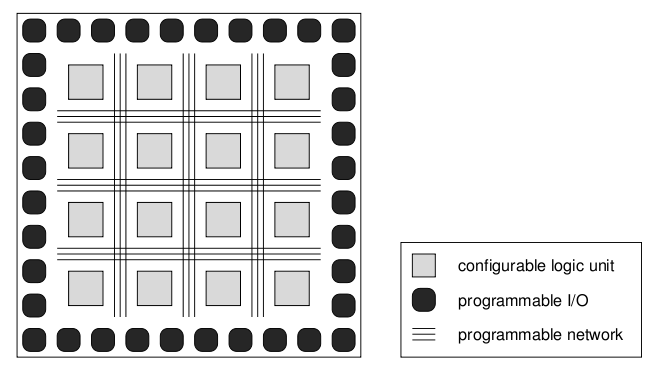
\includegraphics[scale=.50]{./figuras/Fpga.png}
 % capas.png: 607x522 pixel, 72dpi, 21.41x18.41 cm, bb=0 0 607 522
 \caption{FPGA genérico}
 \label{Tarjeta de desarrollo NetFPGA}
\end{figure}



Como uno de los más versátiles componentes de la tecnología VLSI\footnote{VLSI,
es el acrónimo \emph{Very Large Scale Integration}, integración en escala
muy grande. La integración en escala muy grande de sistemas de circuitos basados
en transistores en circuitos integrados comenzó en los años 1980, como parte de
las tecnologías de semiconductores y comunicación que se estaban
desarrollando.}, permite implementar complejos dispositivos electrónicos
diseñados mediante lenguajes de descripción de hardware como VHDL\footnote{VHDL,
es el acrónimo que representa la combinación de VHSIC y HDL, donde VHSIC es el
acrónimo de \emph{Very High Speed Integrated Circuit} y HDL es a su vez el
acrónimo de \emph{Hardware Description Language}.} o Verilog\footnote{Verilog es
un lenguaje de descripción de hardware usado para modelar sistemas electrónicos.
El lenguaje, algunas veces llamado \emph{Verilog HDL}, soporta el diseño, prueba
e implementación de circuitos analógicos, digitales y de señal mixta a
diferentes niveles de abstracción.}, además muchos de estos también contienen
dentro de sí diversos elementos como unidades de memoria que van desde simples
\emph{flip-flops} hasta bloques de memoria dinámica más complejos. También
pueden contener multiplicadores, comparadores e incluso procesadores para formar
sistemas programables en chips\cite{nava}.

% 
\section{NetFPGA}

El Proyecto NetFPGA se refiere a un esfuerzo para desarrollar un hardware de
código abierto y la plataforma de software que permite la rápida creación de
prototipos de dispositivos de red. 

NetFPGA se distingue principalmente en dos formas. En primer lugar se encuentra
en su enfoque basado en FPGA para dispositivos de red de creación de prototipos.
Esto permite a los usuarios desarrollar diseños que son capaces de procesar los
paquetes a velocidad de línea, una capacidad general no lograda por los
enfoques basados en \emph{software}. La segunda característica distintiva en el 
NetFPGA es su enfoque en el apoyo a una comunidad de \emph{hardware} de código
abierto y desarrolladores de \emph{software} que puedan compartir y construir
sobre cada uno de los proyectos y los bloques de construcción\cite{netfpga1}.

\begin{figure}[ht]
 \centering
 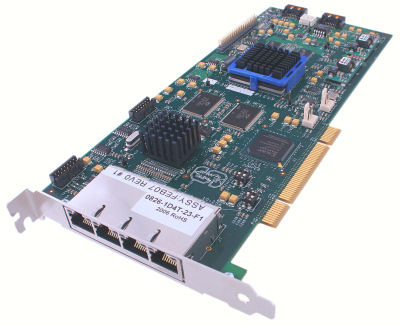
\includegraphics[scale=.50]{./figuras/netfpga.jpg}
 % capas.png: 607x522 pixel, 72dpi, 21.41x18.41 cm, bb=0 0 607 522
 \caption{Tarjeta de desarrollo NetFPGA}
 \label{Tarjeta de desarrollo NetFPGA}
\end{figure}


El NetFPGA incluye el todos los recursos de la lógica, la memoria, y
interfaces Gigabit Ethernet necesarios para construir un \emph{swtich} completo,
el router y  o  un dispositivo de seguridad. Debido a que la ruta de datos
completa se implementa en el hardware, el sistema puede soportar paquetes 
\emph{back-to-back} a velocidad completa de gigabit y tiene una
latencia de procesamiento se mide en sólo unos pocos ciclos de reloj.



Las características con las que cuenta el NetFPGA son:

  \begin{itemize}
   \item Xilinx Virtex-II Pro 50
   \item 4 puertos de red Gigabit Ethernet
   \item 4.5 MBytes SRAM
   \item 64 MBytes DDR2 DRAM
   \item 2 conectores de entrada y salida SATA
   \item Slot PCI Estándar
   \item Conector para cable JTAG Xilinx ChipScope 
  \end{itemize}

\subsection{\emph{PowerPC 405-S Embedded Processor Core}}

El procesador PowerPC 405-S de 32-bits es una implementación de la arquitectura
PowerPC. Es miembro de la familia \emph{PowerPC 400 series}, contiene 
componentes esenciales de un subsistema empotrado de alto rendimiento. Entre
otras funciones incluye memoria gestión, memoria caché y control de
temporizadores y depuración de instalaciones.

La arquitectura del procesador PowerPC 405-S implementa los registros a nivel de
usuario, un modelo de programación, tipos de datos, modos de direccionamiento, y
 32 bits de operaciones de punto fijo. Las operaciones de punto flotante y 
las excepciones que estas causan pueden ser emuladas por software, la
organización del procesador se puede observar en la figura \ref{Organización del
procesador}.

\begin{figure}[ht]
 \centering
 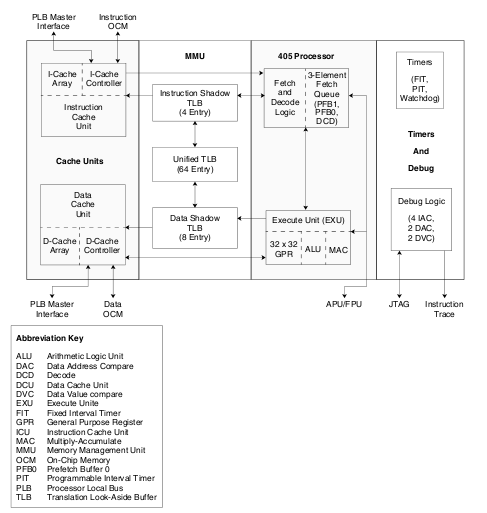
\includegraphics[scale=.60]{./figuras/arc_ppc405.png}
 % capas.png: 607x522 pixel, 72dpi, 21.41x18.41 cm, bb=0 0 607 522
 \caption{Organización del procesador \emph{PowerPC 405-S}}
 \label{Organización del procesador}
\end{figure}


\section{Compilación y carga del \emph{driver} en Linux}

Un controlador de dispositivo, llamado normalmente \emph{driver} es un programa
informático que permite al sistema operativo interactuar con un periférico,
haciendo una abstracción del hardware. Se puede esquematizar como un manual
de instrucciones que le indica al sistema operativo, cómo debe controlar y
comunicarse con un dispositivo en particular. Por tanto, es una pieza esencial,
sin la cual no se podría usar el hardware.

Debido a que el software de controladores de dispositivos se ejecuta como parte
del sistema operativo, con acceso sin restricciones a todo el equipo, resulta
esencial que sólo se permitan los controladores de dispositivos autorizados.

Los \emph{drivers} de la tarjeta de desarrollo NetFPGA se pueden obtener en la
siguiente dirección web:

\url{http://netfpga.org/foswiki/bin/view/NetFPGA/OneGig/Releases}

\subsection{Instalación de dependencias en Debian GNU/Linux}

Dependencia significa que un software necesita de otro para que funcione
adecuadamente. En Linux es común que se necesiten herramientas o librerías para
realizar un trabajo. Este problema se puede resolver, en parte, con programas
que se encargan del software instalado y que tratan de resolver las dependencias
con información proveída por personas encargadas de los paquetes.

En el caso de la tarjeta de desarrollo NetFPGA es necesaria la instalación de
dependencias en el sistema huesped con el fin de poder hacer la compilación del
código fuente del \emph{driver} de forma correcta.

A continuación se listan las dependencias requeridas en Debian GNU/Linux 6.0.4:

\begin{itemize}
 \item \textbf{libncurses5-dev}, este paquete contiene los archivos de
cabecera, bibliotecas estáticas y los enlaces simbólicos que los desarrolladores
que usan ncurses va a necesitar.\\

  \begin{verbatim}
  root@debian:~#apt-get install libncurses5-dev
  \end{verbatim}

 \item \textbf{libnet1-dev}, proporciona un marco portátil de paquete de red de
bajo nivel escritura y manipulación. libnet incluye las interfaces portátiles de
creación de paquetes en la capa IP y la capa de enlace, así como una gran
cantidad de funcionalidad adicional.

  \begin{verbatim}	
  root@debian:~\#apt-get install libnet1-dev
  \end{verbatim}

 \item \textbf{libpcap-dev}, proporciona un marco portátil de bajo nivel
red de monitoreo. Las aplicaciones incluyen estadísticas de la red
recolección, supervisión de la seguridad, la depuración de la red, etc.

  \begin{verbatim}	
  root@debian:~\#apt-get install libpcap-dev
  \end{verbatim}


\end{itemize}


\subsubsection{Compilación del \emph{driver}}

Se compila el \emph{driver}:

  \begin{verbatim}
  root@debian:~\#cd ~/netfpga/  make
  \end{verbatim}

Se instala el \emph{driver}:

  \begin{verbatim}
  root@debian:~#cd ~/netfpga/  make install >> salida_install.txt
  \end{verbatim}

Se reinicia el sistema:

  \begin{verbatim}
  root@debian:~#reboot
  \end{verbatim}

Una vez que el sistema a reiniciado se verifica la carga del \emph{driver}:

  \begin{verbatim}
  root@debian:~#lsmod  | grep nf2 
  nf2                    11925  0 
  \end{verbatim}


 \subsection{Instalación del \emph{driver} en CentOS }
  
Para hacer sencilla la instalación de los \emph{drivers}, se han creado 
paquetes \emph{RPM}\footnote{\emph{ RPM Package Manager} (o \emph{RPM},
originalmente llamado \emph{Red Hat Package Manager}) es una herramienta de
administración de paquetes pensada básicamente para \emph{GNU/Linux}. Es capaz
de instalar, actualizar, desinstalar, verificar y solicitar programas.
\emph{RPM} es el formato de paquete de partida del \emph{Linux Standard Base}.}
y un repositorio de \emph{YUM}\footnote{\emph{Yellow dog Updater, Modified} es
una herramienta libre de gestión de paquetes para sistemas \emph{Linux} basados
en \emph{RPM}.}. Se muestra a continuación los pasos a seguir para la
instalación de la tarjeta de desarrollo NetFPGA en sistemas CentOS y Fedora.

\begin{enumerate}
 \item Ingresar al sistema como usuario \emph{root}
   \begin{verbatim}
  [proyecto@CentOS ~]\$ su -
  Password: 
  [root@CentOS ~]#
  \end{verbatim}
  
 \item Instalar el repositorio \emph{RPMforge}
    \begin{verbatim}
  [root@CentOS ~]#rpm --import http://apt.sw.be/RPM-GPG-KEY.dag.txt
  \end{verbatim}
  
   \item Instalar el paquete descargado
    \begin{verbatim}
  [root@CentOS ~]#rpm -i rpmforge-release-0.5.2-2.el6.rf.*.rpm
  \end{verbatim}
  
     \item Instalar el  repositorio \emph{YUM} NetFPGA 
    \begin{verbatim}
  [root@CentOS ~]#rpm -Uhv
http://netfpga.org/yum/el5/RPMS/noarch/netfpga-repo-1-1_CentOS5.noarch.rpm 
  \end{verbatim}
  
       \item Instalar los paquetes base para la  NetFPGA 
    \begin{verbatim}
  [root@CentOS ~]#yum -y install netfpga-base
  \end{verbatim}
  
  \begin{itemize}
   \item NOTA: Es necesario instalar algunas dependencias para el correcto
funcionamiento de la tarjeta de desarrollo, YUM se encargará de instarlas
automáticamente durante este proceso.
  \end{itemize}  
\end{enumerate}

\subsubsection{Verificando la interfaces de la tarjeta de desarrollo NetFPGA}

Para comprobar que las cuatro interfaces \textbf{nf2cX} se han cargado
correctamente se utiliza el comando :

  \begin{verbatim}
  root@CentOS:~# ifconfig -a | grep nf2 
  nf2c0     Link encap:Ethernet  HWaddr 00:4e:46:32:43:00  
  nf2c1     Link encap:Ethernet  HWaddr 00:4e:46:32:43:01  
  nf2c2     Link encap:Ethernet  HWaddr 00:4e:46:32:43:02  
  nf2c3     Link encap:Ethernet  HWaddr 00:4e:46:32:43:03  
  \end{verbatim}

  
 \subsubsection{Reprogramando CPCI}
 
Una vez instalada la tarjeta de desarrollo en el sistema huesped se debe de
reprogramar el \emph{bus} \emph{CPCI} de la siguiente manera:

  \begin{verbatim}
  root@CentOS:~# /usr/local/sbin/cpci_reprogram.pl --all  
  \end{verbatim}
  
 Esperando la salida:
 
   \begin{verbatim}
   Loading the CPCI Reprogrammer on NetFPGA 0   
   Loading the CPCI on NetFPGA 0   
   CPCI on NetFPGA 0 has been successfully reprogrammed 
  \end{verbatim}
 
 Es necesario reprogramar el \emph{CPCI} cada vez que se inicie el sistema
huesped, esto se puede lograr de forma automatica agregando la siguiente liena
al archivo \emph{/etc/rc.local}:

   \begin{verbatim}
/usr/local/netfpga/lib/scripts/cpci_reprogram/cpci_reprogram.pl --all 
  \end{verbatim}
  

Con el fin de familiarizarse con la tarjeta de desarrollo durante la realizacón
del proyecto se realizaron varias pruebas con proyectos realizados
anteriormente por la comunidad de desarrolladores, estas pruebas se encuentran
documentadas en el \emph{Apéndice \ref{ApexB}}.             


% \section{XUPV5}

En este proyecto se usa la tarjeta Xilinx University Program Virtex 5 (XUPV5).
La tarjeta de desarrollo \emph{XUPV505} es un dispositivo con características
para la evaluación de proyectos de  propósito general, la plataforma de
desarrollo cuenta con memoria incrustrada e interfaces estándar de la industria
de conectividad. Cuenta con el dispositivo FPGA \emph{Virtex-5}.

\subsection{Características de la  tarjeta de desarrollo \emph{XUPV505} }

Las características con las que cuenta la tarjeta de desarrollo son:

\begin{itemize}
 \item FPGA Xilinx \emph{Virtex-5}  
 \item Dos Xilinx XCF32P Flash PROMs (32 Mbyte cada uno) para
configuraciones del dispositivo
 \item Xilinx SystemACE Compact Flash para configuraciones de control
 \item 64-bit 256Mbyte DDR2 small outline DIMM (SODIMM)
 \item 10/100/1000  Interfaces Ethernet 
 \item Intrefaz USB
 \item Sistema de reloj programable
 \item Puerto RS-232
\end{itemize}


\begin{figure}[h!]
 \centering
 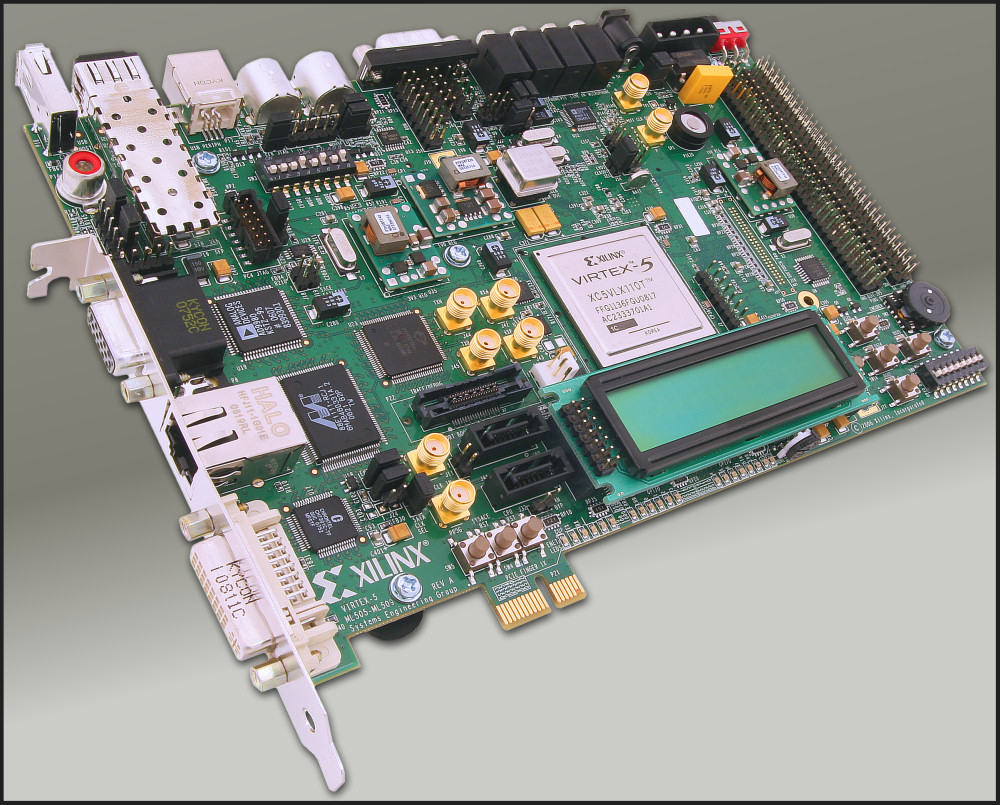
\includegraphics[scale=.30]{./figuras/V5.jpg}
 % V5.jpg: 1000x805 pixel, 72dpi, 35.28x28.40 cm, bb=0 0 1000 805
  \caption{Tarjeta de desarrollo XUPV505}
 \label{XUPV505}
\end{figure}

\section{XUPV2}

En este proyecto se usa la tarjeta Xilinx University Program Virtex 2 (XUPV2).
La tarjeta de desarrollo \emph{XUPV2} es un dispositivo con características
para la evaluación de proyectos de  propósito general, la plataforma de
desarrollo cuenta con memoria incrustrada e interfaces estándar de la industria
de conectividad. Cuenta con el dispositivo FPGA \emph{Virtex-2}.

\subsection{Características de la  tarjeta de desarrollo \emph{XUPV2} }

Las características con las que cuenta la tarjeta de desarrollo son:

\begin{itemize}
\item FPGA Virtex-2 Pro XC2VP30  con 30,816 celdas lógicas, 136 18-bit multiplicadores,
 2,448Kb bloques de RAM y 2 Procesadores PowerPC.
\item DDR SDRAM DIMM de hasta  2Gbytes de RAM
\item Puerto Ethernet 10/100
\item Puerto USB2 
\item Lector de tarjetas Compact Flash
\item Puerto de video XSGA
\item Audio Codec
\item Puertos SATA, S/2 y RS-232
\end{itemize}


\begin{figure}[h!]
 \centering
 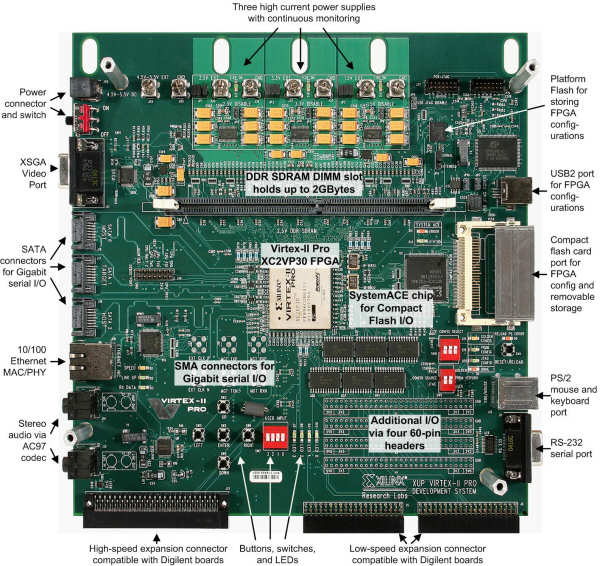
\includegraphics{./figuras/V2.jpg}
 % V5.jpg: 1000x805 pixel, 72dpi, 35.28x28.40 cm, bb=0 0 1000 805
  \caption{Tarjeta de desarrollo Virtex-II Pro Development System}
 \label{XUPV502}
\end{figure}


La lista detallada de características de la tarjeta de desarrollo \emph{XUPV2}
puede ser consultada en la dirección : 
\begin{center}
 \url{http://www.xilinx.com/univ/xupv2p.html}
\end{center}


 





% \chapter{MicroBlaze}

La tarjeta de desarrollo \emph{XUPV5} soporta procesadores
denomimados \emph{softcores} como el procesador
MicroBlaze\footnote{Microblaze es un \emph{soft processor} descrito en VHDL,
es una herramienta muy potente para desarrollar proyectos relacionados con
arquitecturas paralelas, codiseño, control y en toda investigación
sobre software y estudio de metodologías de desarrollo.} de
Xilinx, estos procesadores son descritos en VHDL o Verylog.

\section{Arquitectura MicroBlaze}

El procesador MicroBlaze de 32 bits ha sido desarrollado con unos requisitos muy
estrictos de ocupación y prestaciones, debido a la limitación de los recursos
disponibles en una FPGA. Soluciones arquitectónicas, como la supeescalaridad o
la supersegmentación no resultan adecuadas en un entorno lógico reprogramable,
cuando el objetivo es un diseño compacto. Del mismo modo, la frecuencia de
operación final se ve limitada por los retardos de interconexión en la FPGA.

\begin{figure}[h!]
 \centering
 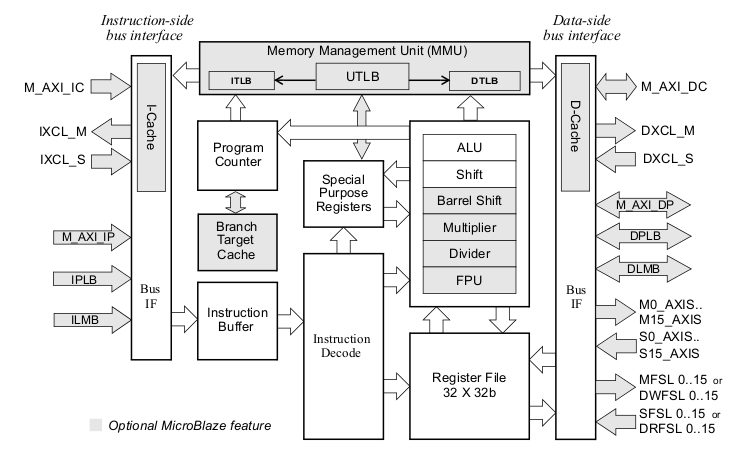
\includegraphics[scale=.55]{./figuras/ublaze.png}
 % ublaze.png: 743x451 pixel, 72dpi, 26.21x15.91 cm, bb=0 0 743 451
   \caption{Diagrama de bloques MicroBlaze}
 \label{MicroBlaze}
\end{figure}

\subsection{Conjunto de instrucciones}

La restricción de espacio fuerza a un diseño sencillo, que encaja perfectamente
con la idea de las arquitecturas tipo RISC\footnote{RISC, acrónimo de \emph{
reduced instruction set computer} es un tipo de diseño de CPU utilizado en
microprocesadores que tienen instrucciones de tamaño fijo y presentadas en un
reducido número de formatos y sólo las instrucciones de carga y almacenamiento
acceden a la memoria de datos.}, donde el limitado número de
instrucciones permite simplificar la unidad de descodificación. En el caso de
MicroBlaze, el número total de instrucciones que soporta son 87, si se
consideran diferentes las instrucciones que operan con valores inmediatos de
aquellas que realizan la misma operación con registros. Adicionalmente, cada
instrucción se ha elegido para que el tamaño de la ALU también sea reducido. Las
instrucciones que requieran un procesamiento complejo habrán de realizarse en un
hardware específico, diseñado utilizando los restantes recursos de la FPGA. El
mecanismo de conexión de estos co-procesadores con Microblaze se especifica en
el protocolo FSL(\emph{Fast Simplex Link}).

\subsection{Pipeline}


Una arquitectura RISC aumenta fácilmente su rendimiento por medio de la
segmentación \emph{pipeline}\footnote{\emph{Pipeline}, consiste en ir
transformando un flujo de datos en un proceso comprendido por varias fases
secuenciales, siendo la entrada de cada una la salida de la anterior.}. En el
caso de MicroBlaze, el número de etapas de pipeline es 3, ejecutando una
instrucción por ciclo de reloj. Como contrapartida, la segmentación debe
incorporar mecanismos para evitar los problemas relacionados con los saltos de
programa. En un salto, la pila está llena de instrucciones que no corresponden
con el flujo de ejecución.

\begin{figure}[h!]
 \centering
 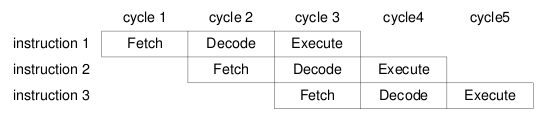
\includegraphics[scale=.60]{./figuras/ciclo.png}
 % ciclo.png: 559x121 pixel, 72dpi, 19.72x4.27 cm, bb=0 0 559 121
    \caption{3 Etapas de \emph{Pipeline: Fetch, Decode y Execute}}
 \label{Ciclo Fetch}
\end{figure}


Estos riesgos están tratados por hardware en MicroBlaze: cada vez que se produce
un salto, el pipeline se vacía cuando el salto se hace efectivo. En el
repertorio se incluyen un cierto número de instrucciones de salto que permiten
la ejecución de la instrucción que les precede, con el objetivo de reducir la
penalización de vaciado. Esta técnica es conocida como \emph{Delay Slots}.

\subsection{Registros Internos y Caché}

Las FPGAs actuales disponen de memoria distribuida con un tiempo de acceso
corto, cuando son utilizadas por la lógica cercana. Este tipo de memoria es
utilizada por MicroBlaze para materializar sus 32 registros internos, el
contador de programa y el registro de estado. Este último sólo contiene el bit
de acarreo, habilitación de cachés, indicador de estado de parada
(\emph{break}), error en el FSL y bit de excepción producida por división por
cero. Además de estos registros internos, MicroBlaze utiliza un buffer de 16
instrucciones mapeado en los registros de desplazamiento. Este recurso es
fundamental para un buen rendimiento del procesador. Por ejemplo, en caso de que
no disponer de multiplicador y/o divisor hardware, se aprovecha el tiempo que
tarda en ejecutarse esta instrucción (32 ciclos) para tener preparadas las
siguientes instrucciones.

La utilización de cachés es una práctica habitual en arquitecturas modernas; el
diseño de MicroBlaze no es una excepción. Pero en este caso, la utilización y
configuración de los tamaños de caché pueden ser fijados por el usuario. Para
ello, existe el siguiente conjunto de opciones a la hora de configurar el
procesador: habilitación de caché de instrucciones y/o datos, tamaño, rango de
direcciones y tamaño de palabra, aunque esta ultima opción solo es valida para
la caché de datos. Opciones no configurables por el usuario son tamaño
de los bloques de caché, la política de sustitución de bloques o el grado de
asociatividad de la caché.

Todas estas opciones se especifican antes de sintetizar el diseño. Las cachés
son de tipo asociativo, por lo cual es necesario el calcular el número de bits
de la dirección (\emph{tag bits}) que especifican bloques contenidos en caché,
mediante la siguente ecuación:
$$ tag bits = log_2(memoriacacheable) - log_2(tamañocaché) $$

Las cachés utilizan los bloques de RAM fijos (BRAM) que contiene la FPGA. Sin
embargo, códigos compactos también pueden mapearse en BRAM. Por lo tanto, la
utilización de cachés será necesaria en aquellos casos donde el código o los
datos utilizado por MicroBlaze residan fuera de la FPGA.

\subsection{Buses del Sistema}

MicroBlaze sigue el modelo de arquitectura Harvard, donde datos e instrucciones
son almacenados en memorias diferentes. De nuevo, gracias a la capacidad de
reconfiguracion de las FPGAs, es posible configurar el sistema con diferentes
opciones sobre los buses, pudiéndose reducir de este modo el tamaño final del
sistema. MicroBlaze utiliza el estándar \emph{CoreConnect} creado por IBM, para
conectar diferentes elementos en un circuito integrado. Un aspecto interesante
es que \emph{CoreConnect} permite reducir la carga capacitiva del bus,
repartiéndola entre varios buses. Así, se consiguen mayores rendimientos, dado
que los retardos de pistas globales son muy importantes en FPGAs.

El estándar define tres tipos de buses, cada uno con unas características de
velocidad y conectividad:

\begin{itemize}
 \item LMB (\emph{Local Memory Bus}): Bus síncrono de alta velocidad, utilizado
para conectar periféricos y los bloques de memoria interna de la FPGA. Solo
admite un maestro en su implementación para MicroBlaze y puede ser utilizado
tanto para instrucciones como para datos. Este bus es compatible con el PLB
(\emph{Processor Local Bus}) incluido en el estándar \emph{CoreConnect}, pero a
diferencia de éste, el LMB no admite varios maestros ni tamaños de palabra
diferentes a 32 bits.
 
  \item OPB (\emph{On-chip Peripheral Bus}): Bus síncrono utilizado para
conectar periféricos con tiempos de acceso variables. Soporta varios maestros y
la conectividad de muchos periféricos es sencilla gracias a su identificación
por multiplexación distribuida. Soporta transferencias de tamaño de palabra
dinámico.

 \item 	DCR (Device Control Register): Bus síncrono diseñado para una conexión
tipo anillo de periféricos con ancho de banda muy bajo. Solo soporta un maestro
y está diseñado para minimizar el uso de lógica interna.
\end{itemize}

Además de estos tres buses existe otra alternativa para comunicarse con el
procesador MicroBlaze. Se trata de un protocolo de comunicación denominado FSL
(\emph{Fast Simplex Link}) mencionado anteriormente, que permite la comunicación
con el procesador a través de sus propios registros internos. El periférico
actuaría a modo de co-procesador y la conexión se realiza de manera sencilla a
través de unos registros de desplazamiento de 32 bits de ancho. La comunicación
con estas \emph{FIFOs} se realiza con dos instrucciones específicas del
repertorio, que realizan las funciones de push y pop de estas memorias de
desplazamiento. MicroBlaze soporta hasta 16 dispositivos conectados con este
protocolo.


\subsection{Interrupciones y excepciones}

El procesador MicroBlaze contiene una línea de interrupciones, la cual al ser
activada hace que el procesador ejecute una rutina de manejo de interrupciones
que ha de ser especificada al compilador. Las excepciones se tratan de forma
similar. Cuando una de ellas ocurre, se paraliza el procesamiento de
instrucciones y se ejecuta una rutina de manejo de excepciones. En el caso de
que el sistema necesite manejar más de una interrupción, será necesario la
utilización de un periférico específico (\emph{OPB Interrupt Controller}), que
se encarga de multiplexar e identificar las diferentes fuentes de
interrupción\cite{microblaze}.


















\chapter{Diseño del \emph{hardware}}

\section{Introducción}

\emph{The Embedded Development Kit} (EDK) es un entorno de desarrollo integrado
para el diseño de sistemas empotrados. Este kit preconfigurado incluye
\emph{Xilinx Platform Studio} y el kit de desarrollo de software, así como toda
la documentación e IP que requieren para el diseño de FPGAs con procesadores
PowerPC integrados.

\section{Plataforma de \emph{hardware}}

La plataforma de \emph{hardware}, incluye uno o más procesadores, además de
una variedad de periféricos y los bloques de memoria. Estos bloques utilizan una
red de interconexión para comunicarse. El comportamiento de cada procesador o
núcleo periférico se pueden personalizar\cite{Beto}.


Para el diseño del \emph{hardware} se hará uso de la herramienta \emph{Xilinx
EDK 8.2.02 Build EDK\_Im\_Sp2.4}, para la detalles de la instalación se puede
consultar el \emph{Apéndice A}.

\section{Diseño y configuración del sistema de \emph{hardware}}

\begin{enumerate}
 \item Creación de un nuevo Proyecto, \emph{figura} \ref{Nuevo proyecto en
Xilinx EDK}.
  \begin{figure}[h!] 
  \centering
  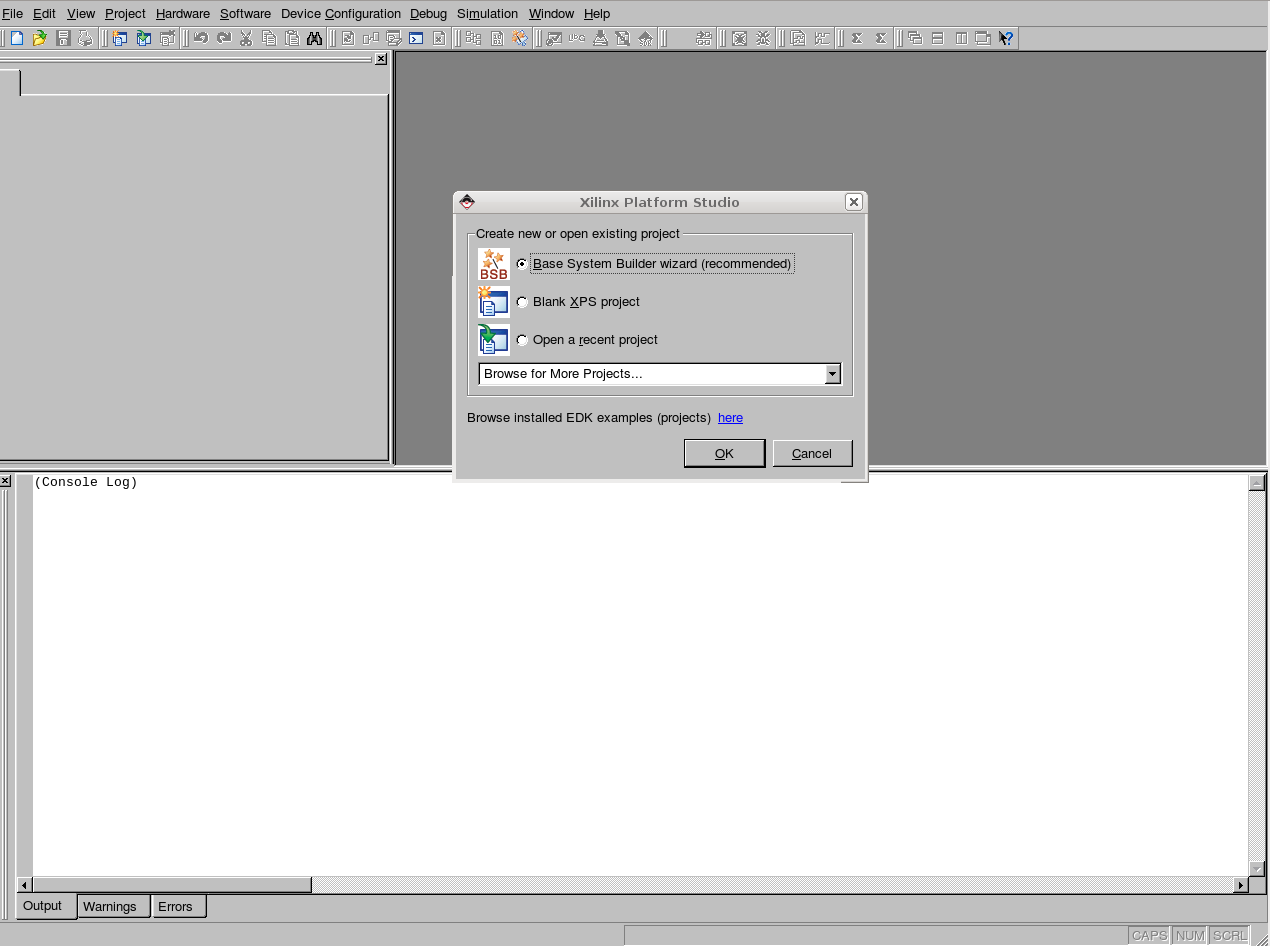
\includegraphics[scale=.25]{./figuras/EDK0.png}
  % capas.png: 607x522 pixel, 72dpi, 21.41x18.41 cm, bb=0 0 607 522
  \caption{Nuevo proyecto en Xilinx EDK}
  \label{Nuevo proyecto en Xilinx EDK}
  \end{figure}
 \item Selección del directorio destino, \emph{figura} \ref{Selección del
directorio destino}.
  \begin{figure}[h!] 
  \centering
  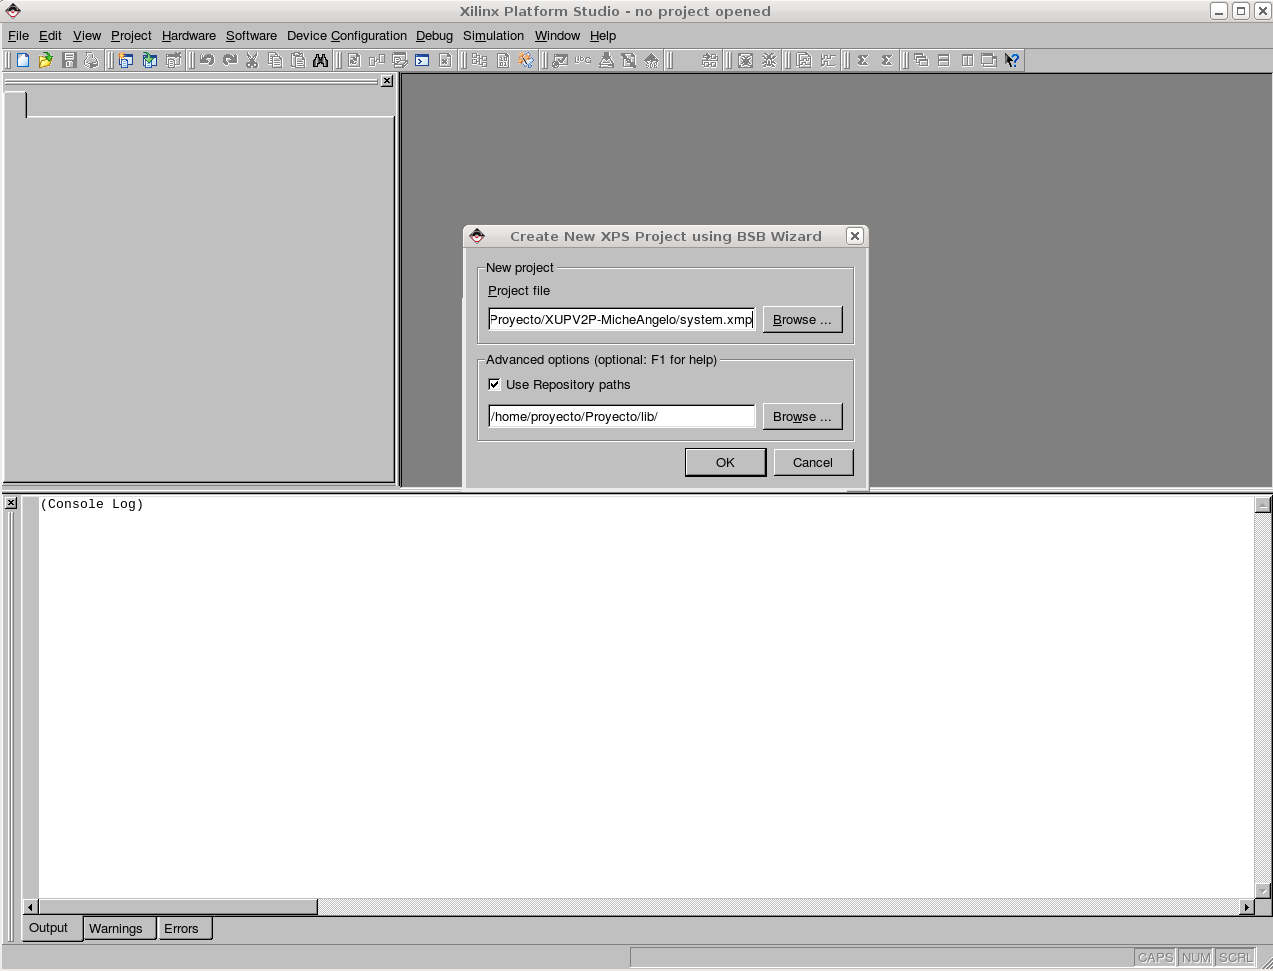
\includegraphics[scale=.25]{./figuras/EDK1.png}
  % capas.png: 607x522 pixel, 72dpi, 21.41x18.41 cm, bb=0 0 607 522
  \caption{Selección del directorio destino}
  \label{Selección del directorio destino}
  \end{figure}
 \item Ajuste del \emph{Project Peripheral Repositories} a los contenidos\\
``lib\_xupv2p\_edk\_10\_1\_sp3.zip'' que puede descargarse de la pagina de
 \emph{diligent}
 \url{http://www.digilentinc.com/Products/Detail.cfm?Prod=XUPV2P}. 
  Este archivo es necesario para que XPS reconozca las características de la
tarjeta, \emph{figura} \ref{Selección del directorio destino}.
 \item Seleccione crear un nuevo diseño con \emph{I would like to create a new
design} como se muestra en la \emph{figura} \ref{Selección de un nuevo diseño}.
  \begin{figure}[h!] 
  \centering
  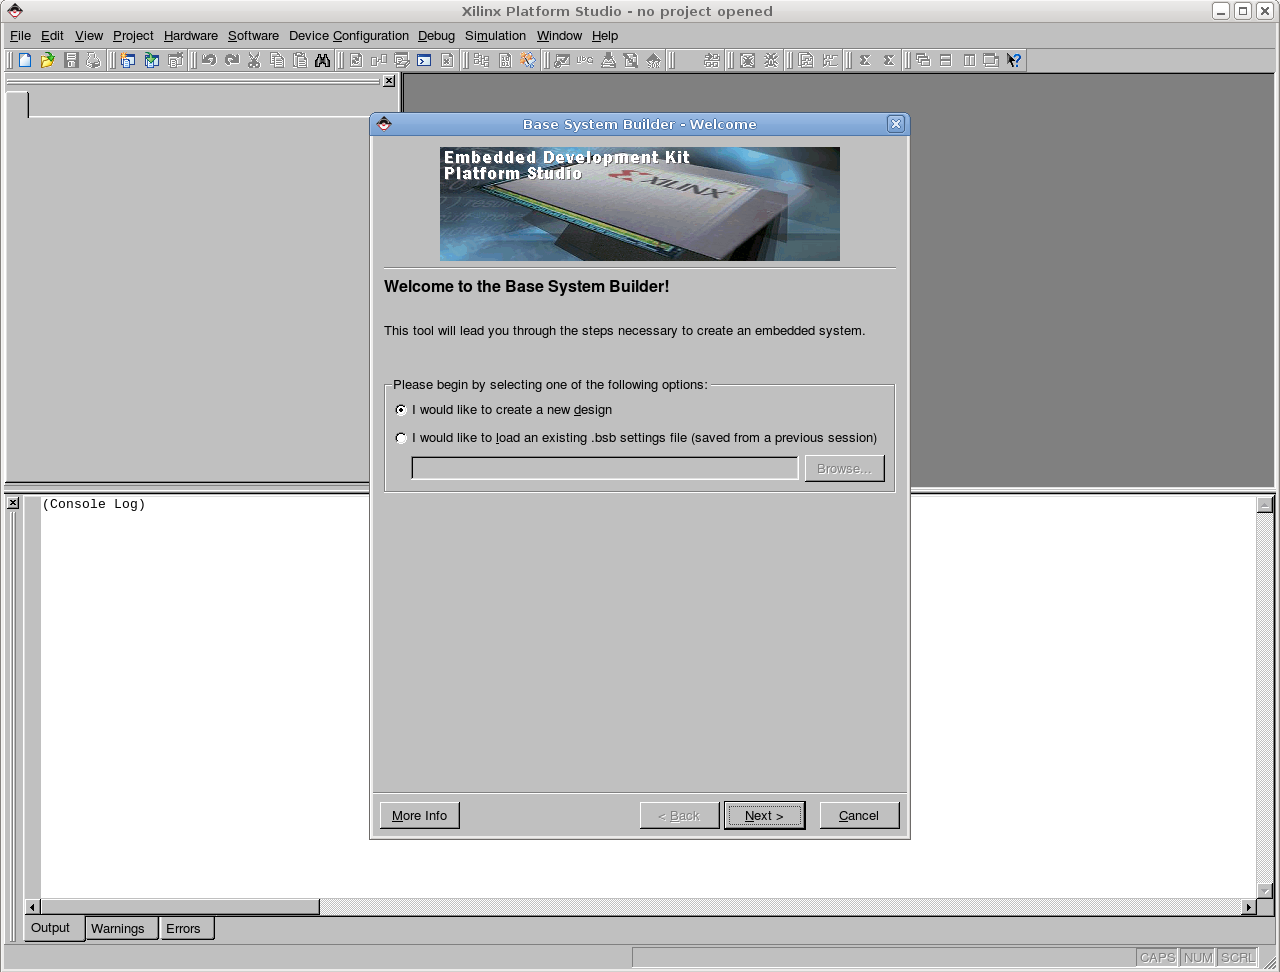
\includegraphics[scale=.25]{./figuras/EDK2.png}
  % capas.png: 607x522 pixel, 72dpi, 21.41x18.41 cm, bb=0 0 607 522
  \caption{Selección de un nuevo diseño}
  \label{Selección de un nuevo diseño}
  \end{figure}
 
  
 \item Seleccione Vendor ``Xilinx'' esto ajustará automáticamente el modelo
 adecuado: ``XUP Virtex-II Pro Development System'', \emph{figura}
\ref{Selección de tarjeta de desarrollo}.
  \begin{figure}[h!] 
  \centering
  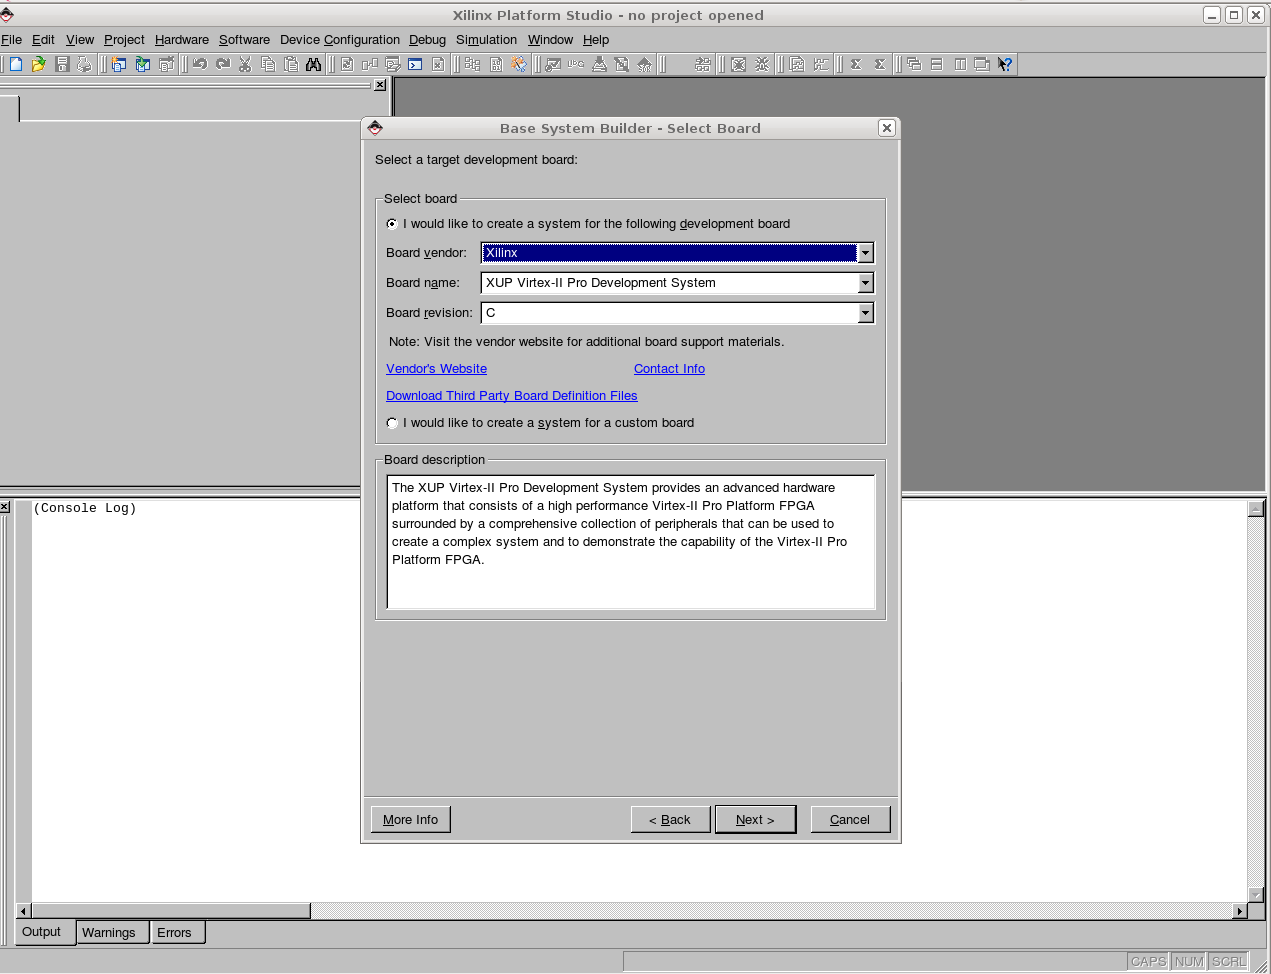
\includegraphics[scale=.25]{./figuras/EDK3.png}
  % capas.png: 607x522 pixel, 72dpi, 21.41x18.41 cm, bb=0 0 607 522
  \caption{Selección de tarjeta de desarrollo}
  \label{Selección de tarjeta de desarrollo}
  \end{figure}
    
  \item Seleccione PowerPC, como se menciona en las características de la
tarjeta de desarrollo la tarjeta XUPV2P cuenta con un procesador PowerPC405 sin
unidad de punto flotante, \emph{figura}
\ref{Selección de procesador}.
  \begin{figure}[h!] 
  \centering
  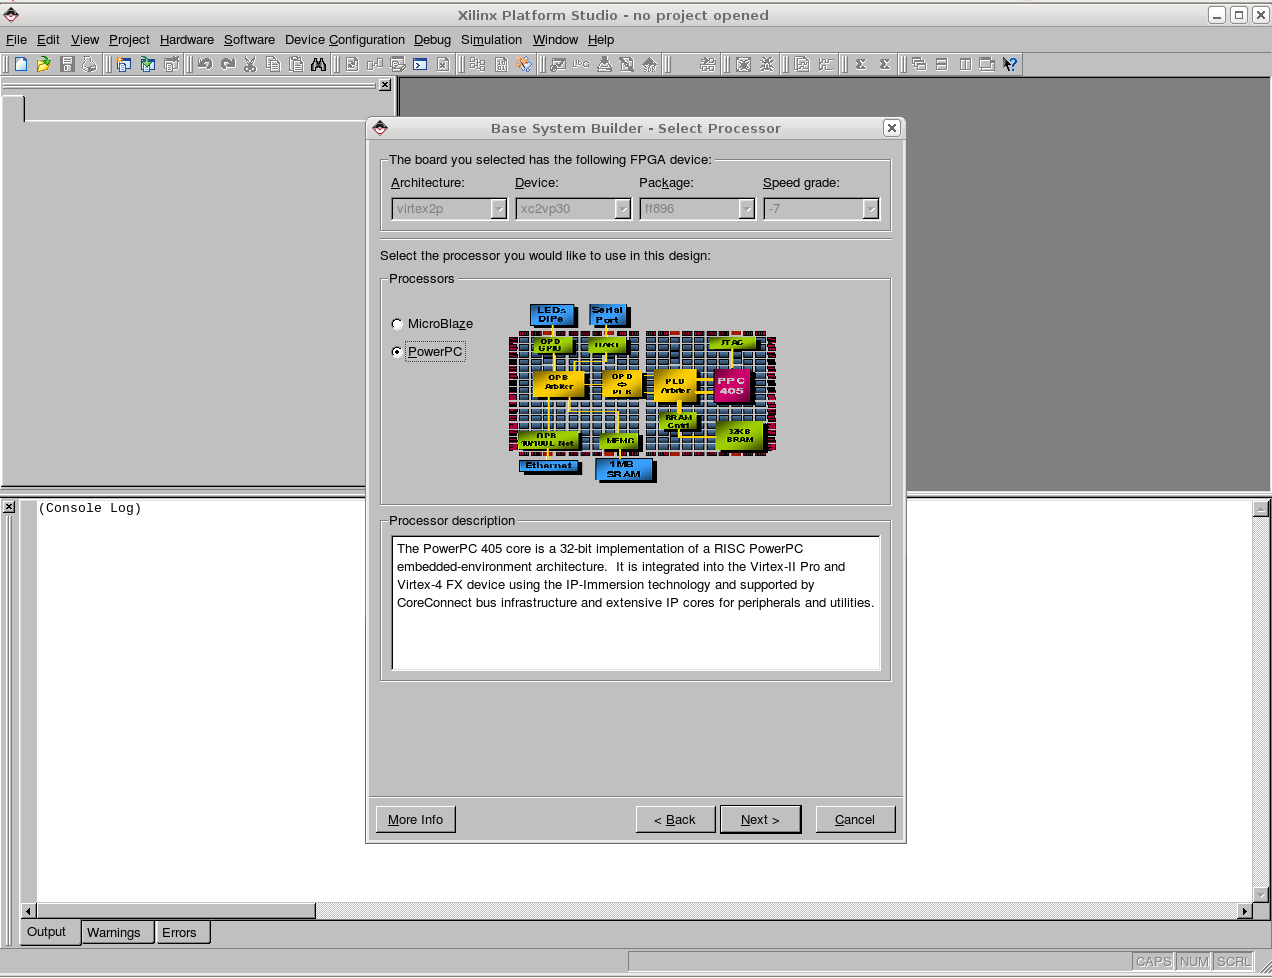
\includegraphics[scale=.25]{./figuras/EDK4.png}
  % capas.png: 607x522 pixel, 72dpi, 21.41x18.41 cm, bb=0 0 607 522
  \caption{Selección de procesador}
  \label{Selección de procesador}
  \end{figure}
 
  
 \item Aumentar la frecuencia de la CPU a 300 MHz. Habilitar la caché. Es
posible aumentar la frecuencia a 400MHz en pasos posteriores, pero requiere
consideraciones especiales y no es posible aumentar la velocidad del bus
principal (100MHz) así que el aumento de la frecuencia no incide
significativamente en el rendimiento, \emph{figura}
\ref{Configurando el procesador PowerPC}.
  \begin{figure}[h!] 
  \centering
  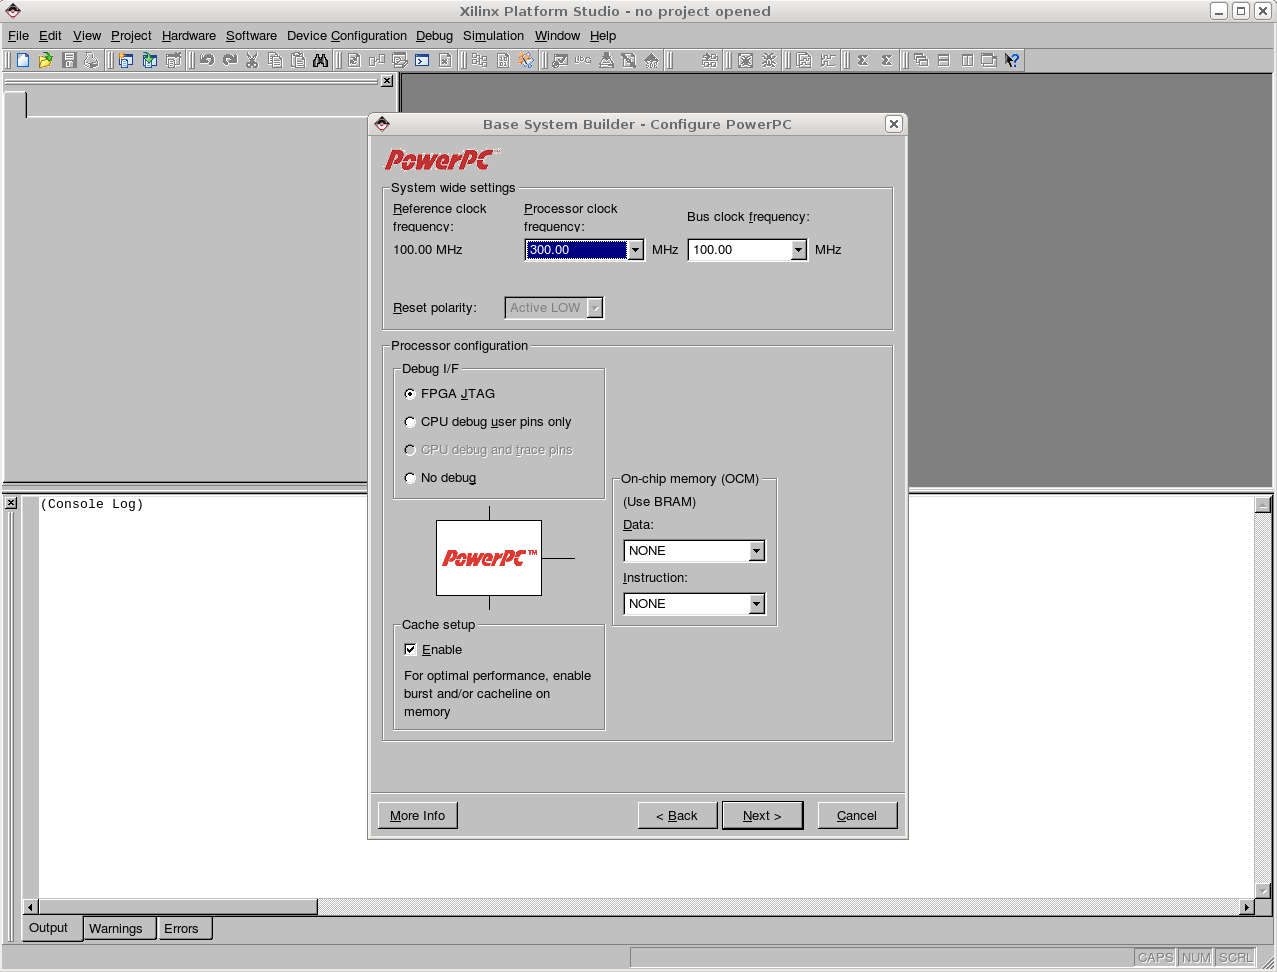
\includegraphics[scale=.25]{./figuras/EDK5.png}
  % capas.png: 607x522 pixel, 72dpi, 21.41x18.41 cm, bb=0 0 607 522
  \caption{Configurando el procesador PowerPC}
  \label{Configurando el procesador PowerPC}
  \end{figure}
  
  
\item Aumentar la velocidad de transmisión RS232 a 9600 Baudios y seleccione
\emph{Use interrupt} para cada periférico. Es posible aumentar la velocidad de
transmisión, esta es la minima recomendada, \emph{figura}
\ref{Configuracón del RS232}.
  \begin{figure}[h!] 
  \centering
  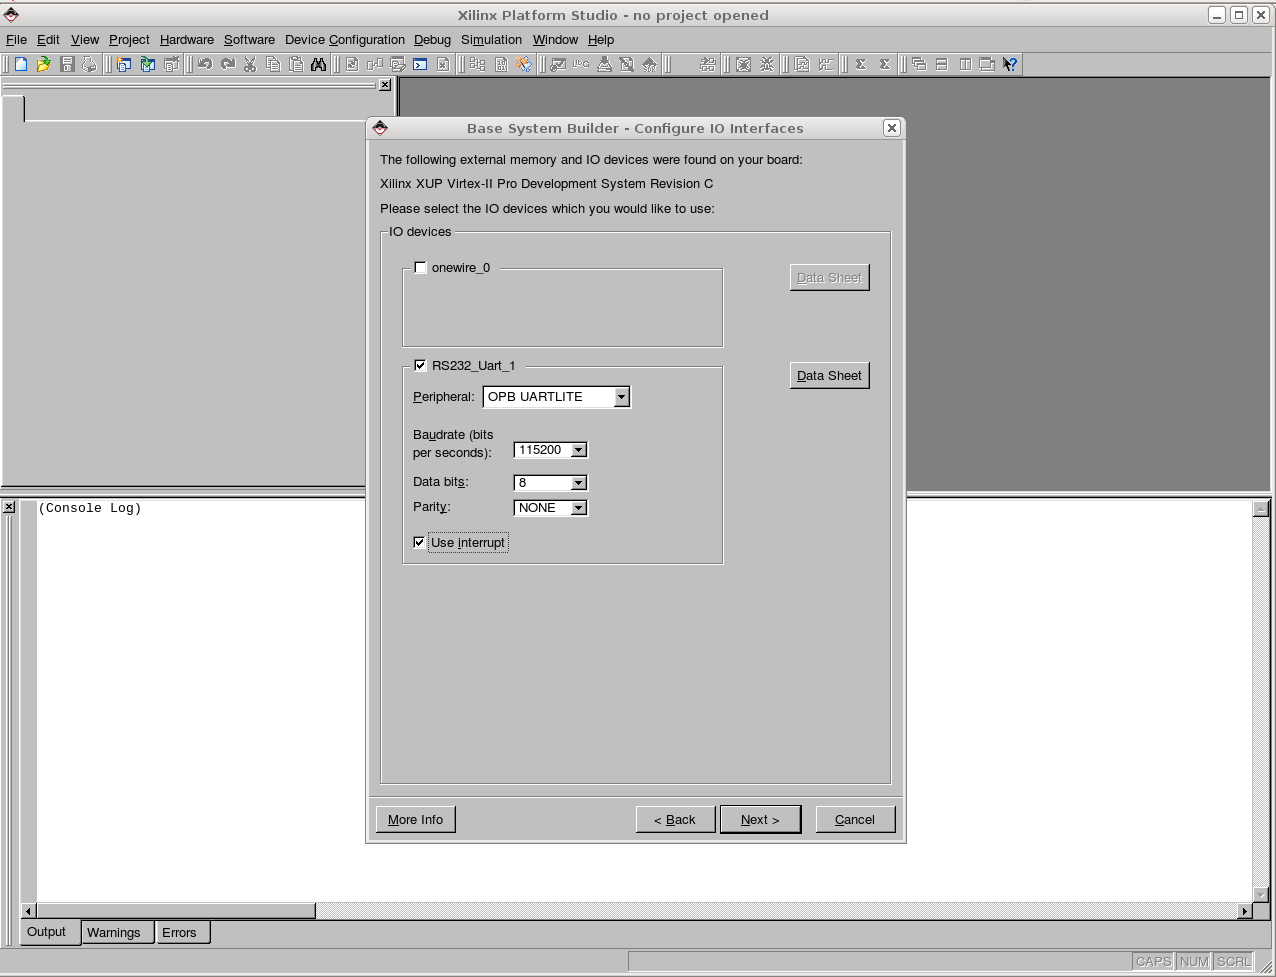
\includegraphics[scale=.25]{./figuras/EDK6.png}
  % capas.png: 607x522 pixel, 72dpi, 21.41x18.41 cm, bb=0 0 607 522
  \caption{Configuracón del RS232}
  \label{Configuracón del RS232}
  \end{figure}
 
   
\item Seleccione ``Ethernet\_MAC'' y seleccione ``OPB ETHERNETLITE'' y Active
interrupción. Este ``OPB ETHERNETLITE'' se puede obtener desde la pagina de la
empresa ``Xilinx'' sin costo alguno, en la  \emph{figura}
\ref{lic} se puede ver el estado de la licencia.
  \begin{figure}[h!] 
  \centering
  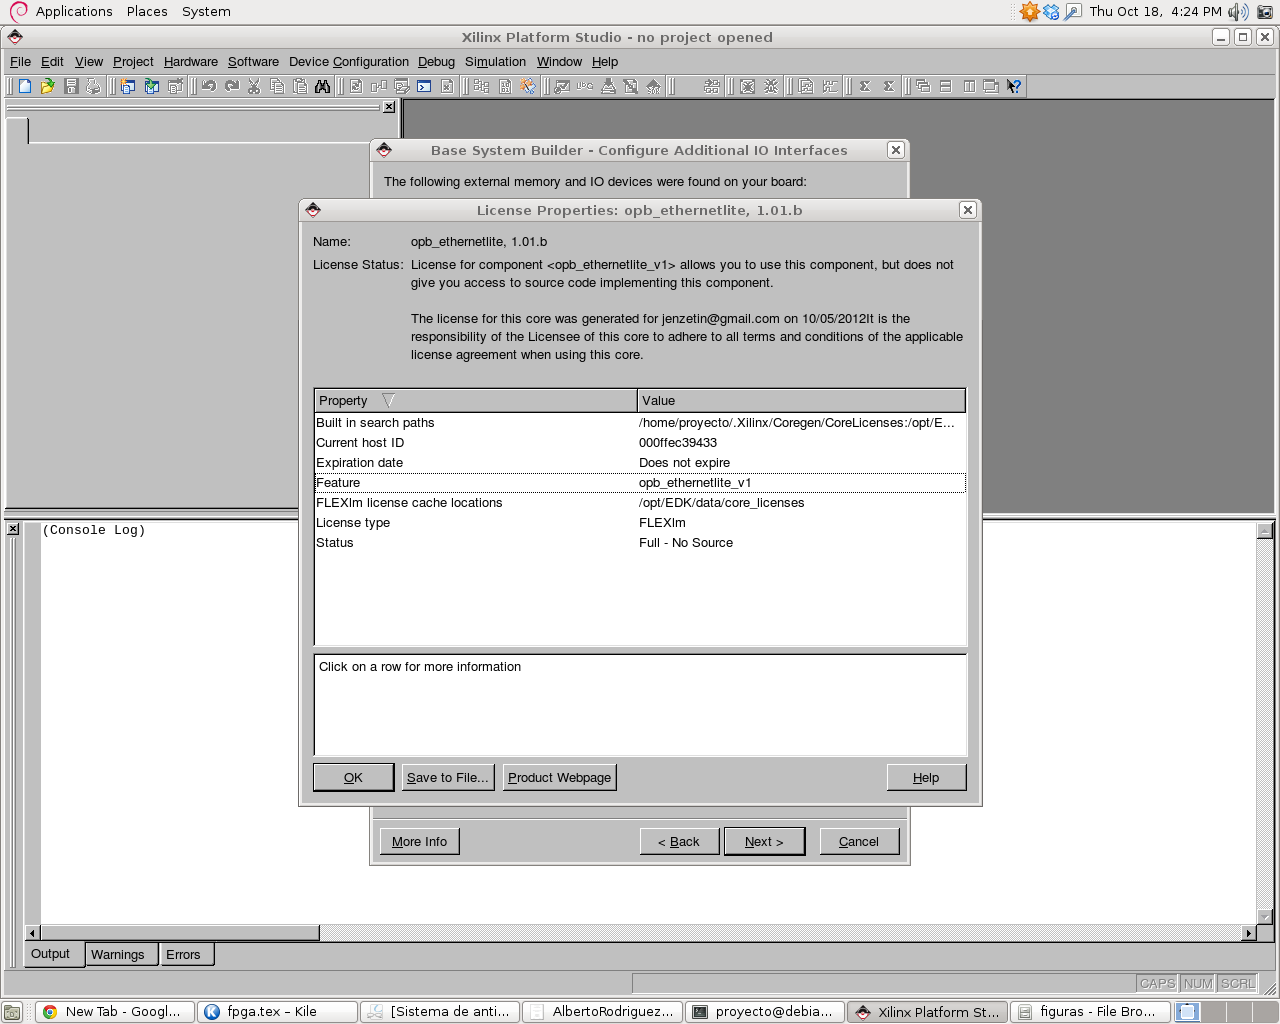
\includegraphics[scale=.25]{./figuras/lic.png}
  % capas.png: 607x522 pixel, 72dpi, 21.41x18.41 cm, bb=0 0 607 522
  \caption{Estado de la licencia}
  \label{lic}
  \end{figure}
  
  
\item Seleccione SysACE\_CompactFlash y active interrupción,  \emph{figura}
\ref{Selección del SysACE}.
  \begin{figure}[h!] 
  \centering
  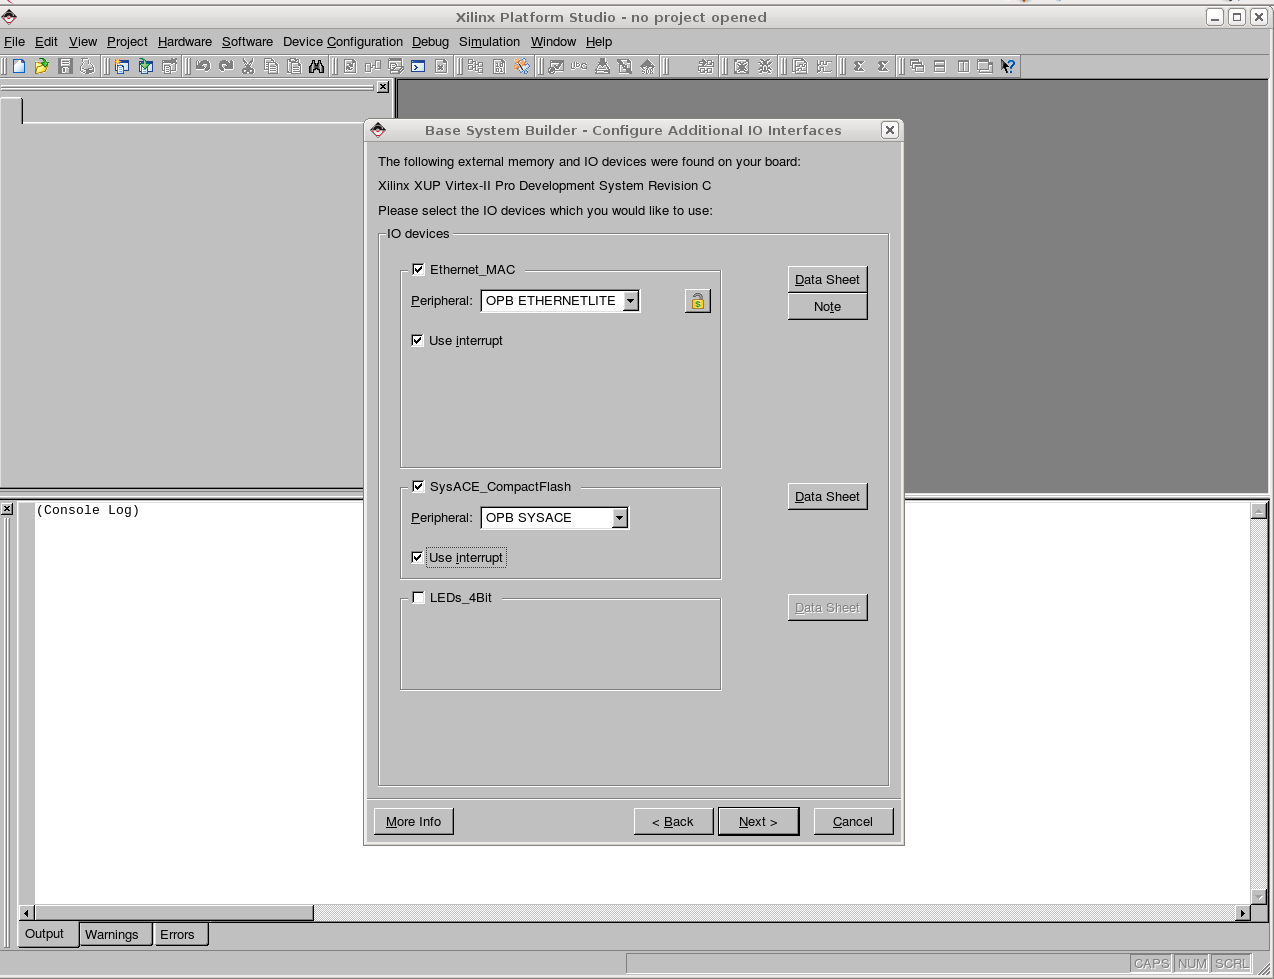
\includegraphics[scale=.25]{./figuras/EDK7.png}
  % capas.png: 607x522 pixel, 72dpi, 21.41x18.41 cm, bb=0 0 607 522
  \caption{Selección del  Ethernet\_MAC y SysACE}
  \label{Selección del SysACE}
  \end{figure}
  
  
\item Seleccione la memoria DDR disponible, en mi caso 256MB. Deseleccione el
resto del hardware. Deseleccione la interrupción,  \emph{figura}\ref{Selección
de Dispositivo de Memoria DDR}.
  \begin{figure}[h!] 
  \centering
  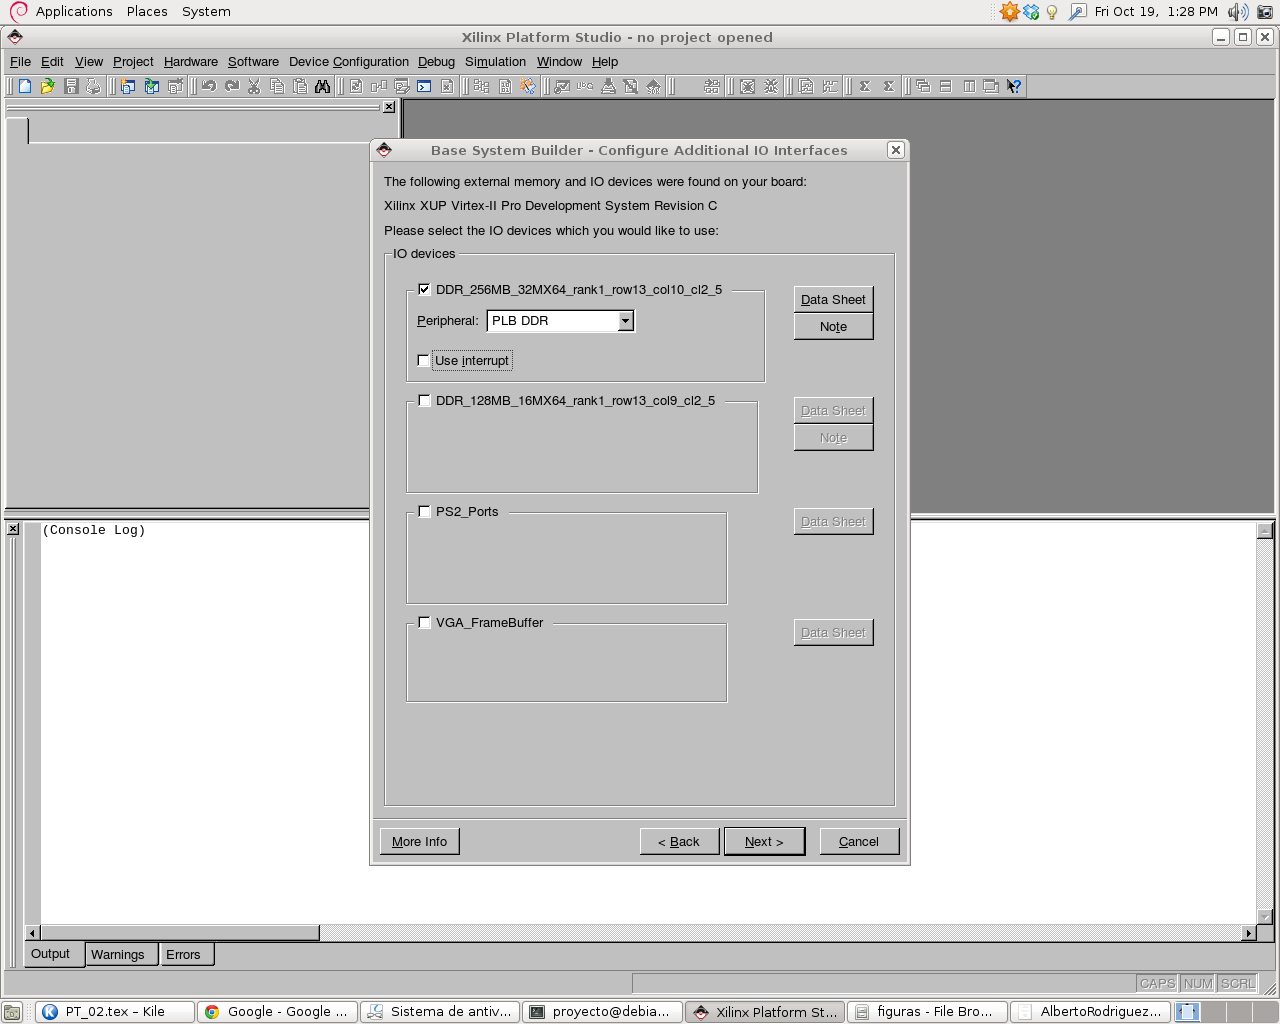
\includegraphics[scale=.25]{./figuras/EDK8.png}
  % capas.png: 607x522 pixel, 72dpi, 21.41x18.41 cm, bb=0 0 607 522
  \caption{Selección de Dispositivo de Memoria DDR}
  \label{Selección de Dispositivo de Memoria DDR}
  \end{figure}
  
  
\item Elija 128 kB de RAM. No elija 8 kB, ya que esto no es compatible con el
Virtex- II PRO. Se debe de contar  con BRAM para que el \emph{bootloop} del
procesador PPC405 funcione correctamente. El \emph{bootloop} es el proceso
mediante el cual procesador busca y carga el programa que ejecutara desde la
dirección \emph{0xfffffffc}, esto se muestra en la
\emph{figura}\ref{Configuracón de BRAM}.
  \begin{figure}[h!] 
  \centering
  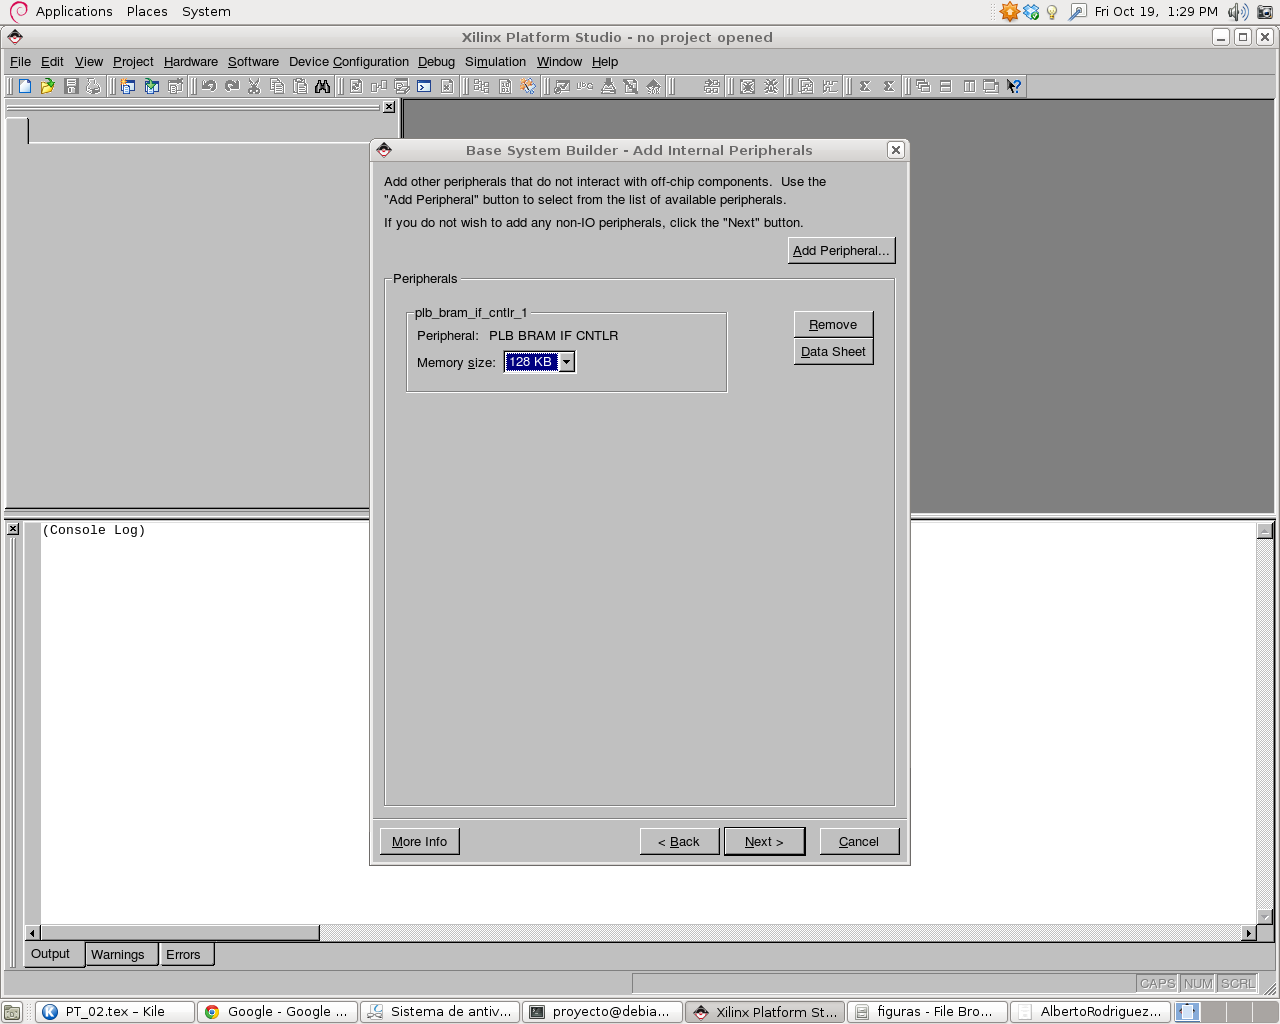
\includegraphics[scale=.25]{./figuras/EDK9.png}
  % capas.png: 607x522 pixel, 72dpi, 21.41x18.41 cm, bb=0 0 607 522
  \caption{Selección de Dispositivo de Memoria DDR}
  \label{Configuracón de BRAM}
  \end{figure}

\item Habilitar ICACHE y DCACHE (Instrucciones y datos respectivamente) para
DDR\_SRAM. En código C de Xilinx esto permite usar las macros
``XCache\_EnableICache'' y ''XCache\_EnableDCache'' para habilitar la cache y
teóricamente aumentar el desempeño, la configuración se mustra en la
\emph{figura}\ref{Selección de lineas de Caché}.
  \begin{figure}[h!] 
  \centering
  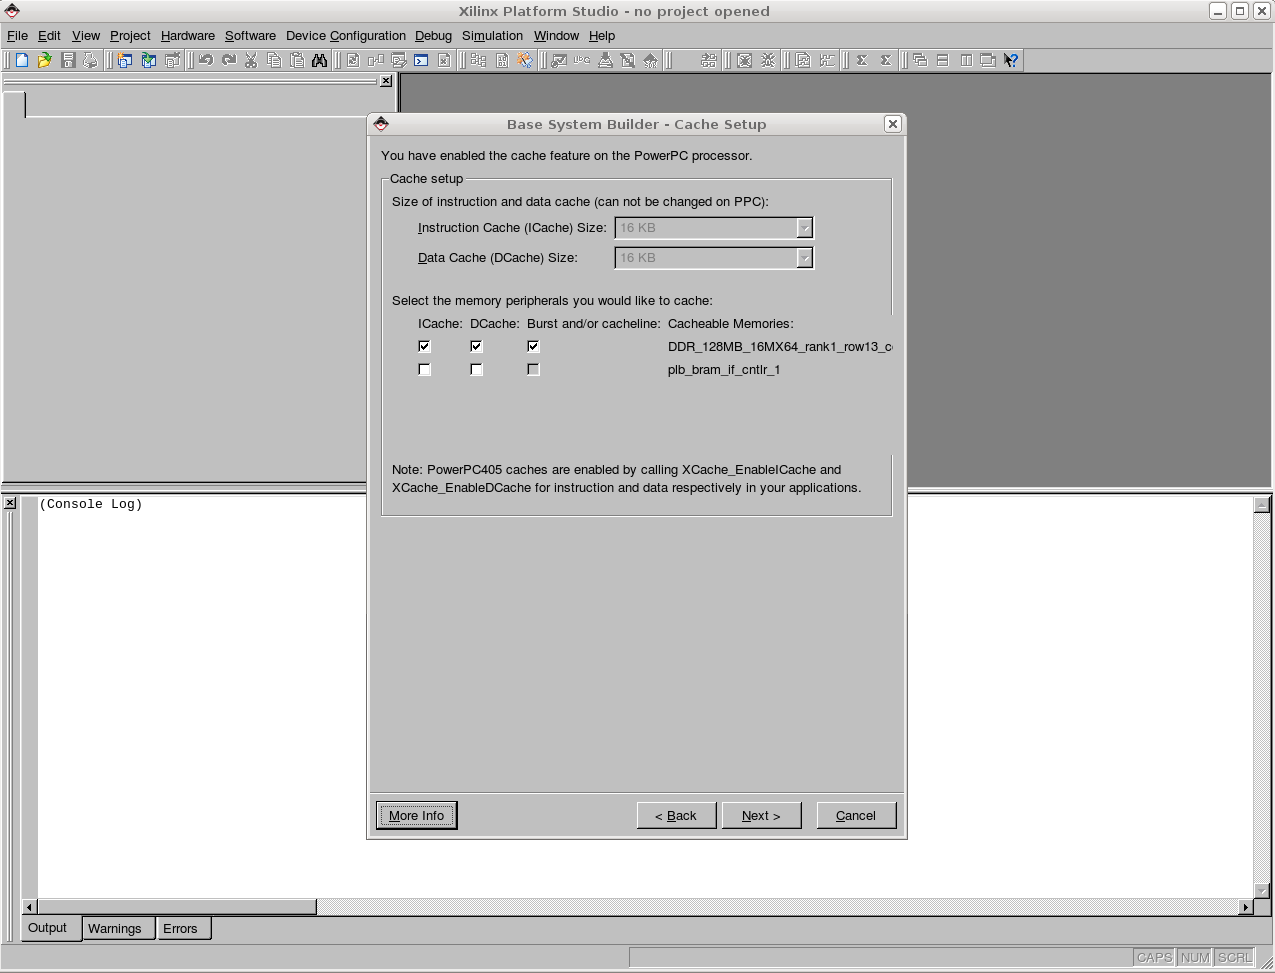
\includegraphics[scale=.25]{./figuras/EDK10.png}
  % capas.png: 607x522 pixel, 72dpi, 21.41x18.41 cm, bb=0 0 607 522
  \caption{Selección de lineas de Caché}
  \label{Selección de lineas de Caché}
  \end{figure}
  
  
\item Seleccione \emph{TestMemory}, \emph{TestMemory} permitirá saber que la
plataforma hardware funciona aunque sea en un nivel muy básico. Ya no es
necesario configurar más \emph{hardware}, esto se muestra en la
\emph{figura}\ref{Selección de programa de prueba}.
  \begin{figure}[h!] 
  \centering
  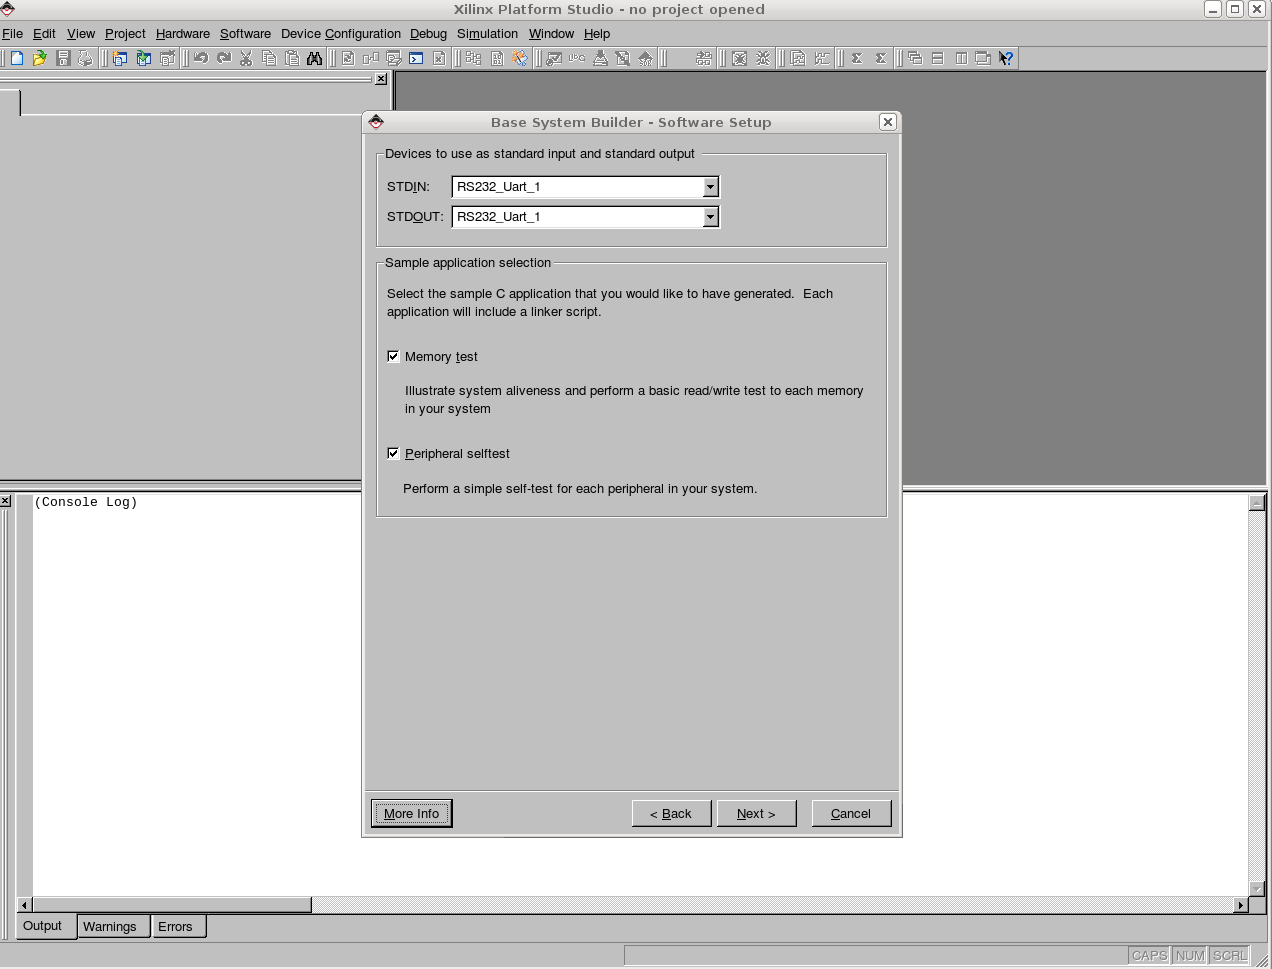
\includegraphics[scale=.25]{./figuras/EDK11.png}
  % capas.png: 607x522 pixel, 72dpi, 21.41x18.41 cm, bb=0 0 607 522
  \caption{Selección de programa de prueba}
  \label{Selección de programa de prueba}
  \end{figure}
  
  
\item Mantenga los datos, instrucciones y \emph{Heap/Stack} en la BRAM. Es
necesario para poder ser alcanzados en el \emph{BootLoop} del PPC405,
\emph{hardware}, esto se muestra en la
\emph{figura}\ref{Selección de división del programa en memoria}.
  \begin{figure}[h!] 
  \centering
  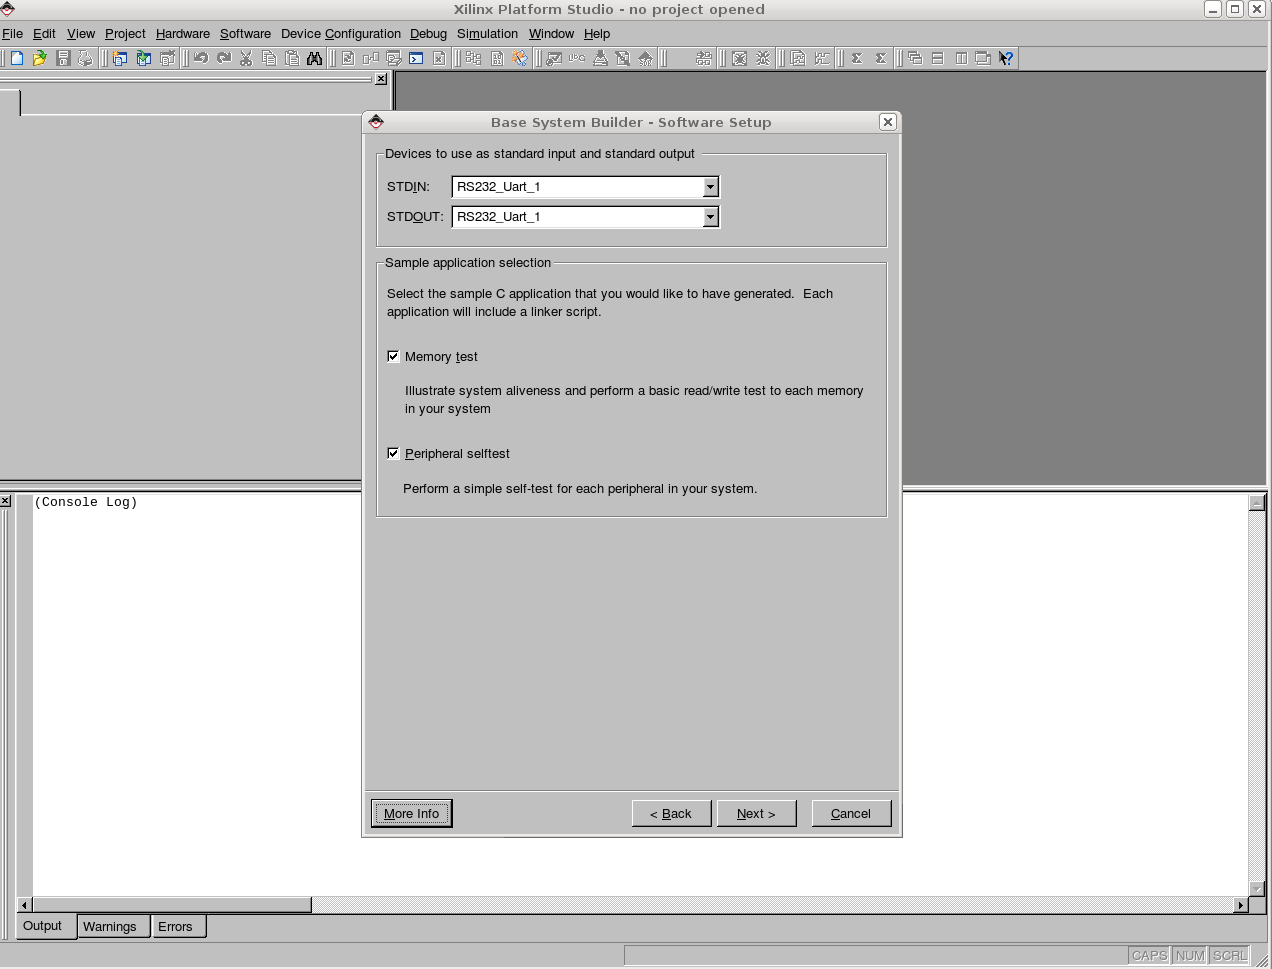
\includegraphics[scale=.25]{./figuras/EDK11.png}
  % capas.png: 607x522 pixel, 72dpi, 21.41x18.41 cm, bb=0 0 607 522
  \caption{Selección de división del programa en memoria}
  \label{Selección de división del programa en memoria}
  \end{figure}
  
  
\item Generación del \emph{hardware}, \emph{figura}\ref{Generación de hardware}.
  \begin{figure}[h!] 
  \centering
  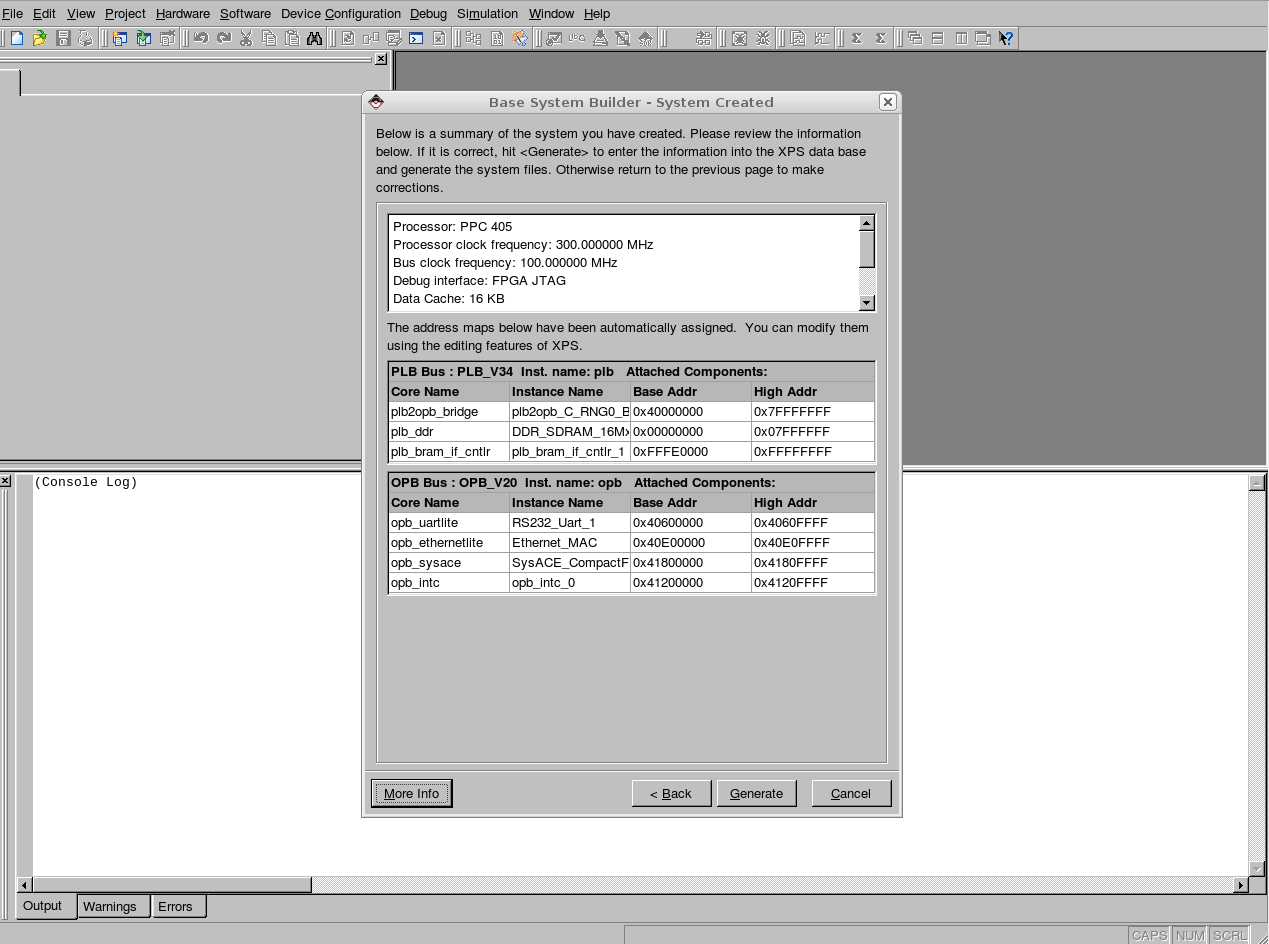
\includegraphics[scale=.25]{./figuras/EDK13.png}
  % capas.png: 607x522 pixel, 72dpi, 21.41x18.41 cm, bb=0 0 607 522
  \caption{Generación de \emph{hardware} }
  \label{Generación de hardware}
  \end{figure}
  
  
\item El siguiente paso es activar el doble buffer (también conocido como
``ping-pong'' buffers) para el núcleo opb\_ethernetlite (doble clic sobre
``Ethernet\_MAC'' de la \emph{``System Assembly View''}),
\emph{figura}\ref{Configuración del OPB EthernetLite}.
  \begin{figure}[h!] 
  \centering
  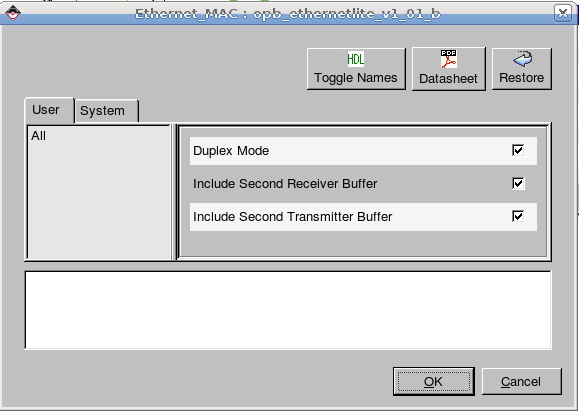
\includegraphics[scale=.25]{./figuras/pingpong.png}
  % capas.png: 607x522 pixel, 72dpi, 21.41x18.41 cm, bb=0 0 607 522
  \caption{Configuración del OPB\_EthernetLite}
  \label{Configuración del OPB EthernetLite}
  \end{figure}
  
  
\item Generación del proyecto( Opción de menú: \emph{``Device Configuration:
Update Bistream''}).
\item Habilite el \emph{bootloop} en la BRAM, dando click derecho en pestaña de
aplicaciones y seleccionando \emph{``Mark to initialize BRAM''},
\emph{figura}\ref{Confuración del bootloop}.
  \begin{figure}[h!] 
  \centering
  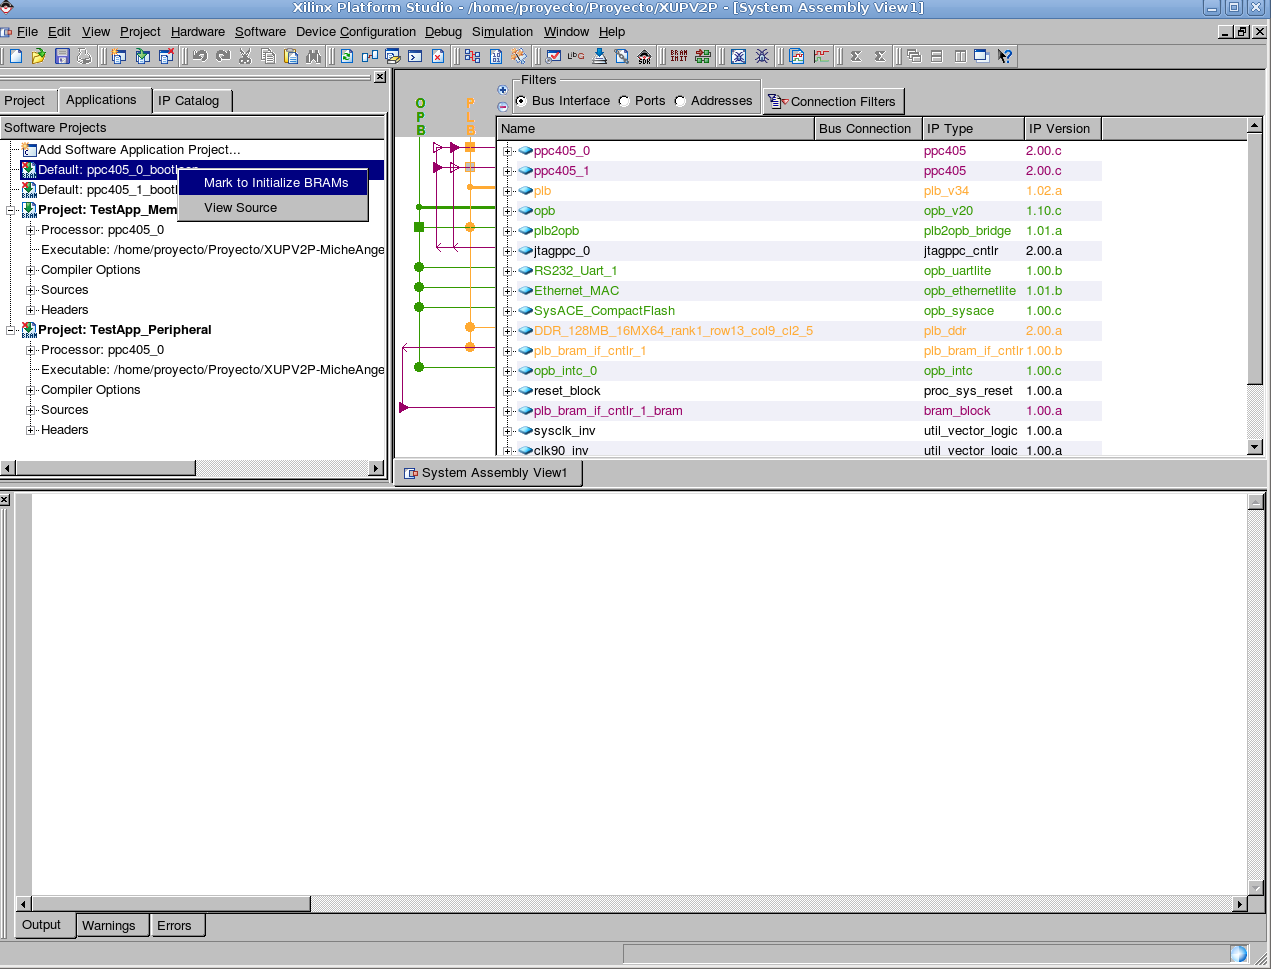
\includegraphics[scale=.25]{./figuras/bootloop.png}
  % capas.png: 607x522 pixel, 72dpi, 21.41x18.41 cm, bb=0 0 607 522
  \caption{Confuración del bootloop}
  \label{Confuración del bootloop}
  \end{figure}

\item Generar el árbol de dispositivos de Linux. Cuando haya terminado de
ejecutar el software de pruebas básicas, es hora de volver a configurar el
software en el proyecto de XPS para generar un árbol de dispositivos, necesario
para compilar un kernel de Linux a la medida. 

\item   Menú ``Software: Software Platform Settings...'' a
continuación, seleccione ``device-tree``, como el sistema operativo,
\emph{figura}\ref{devicetree}.
  \begin{figure}[h!] 
  \centering
  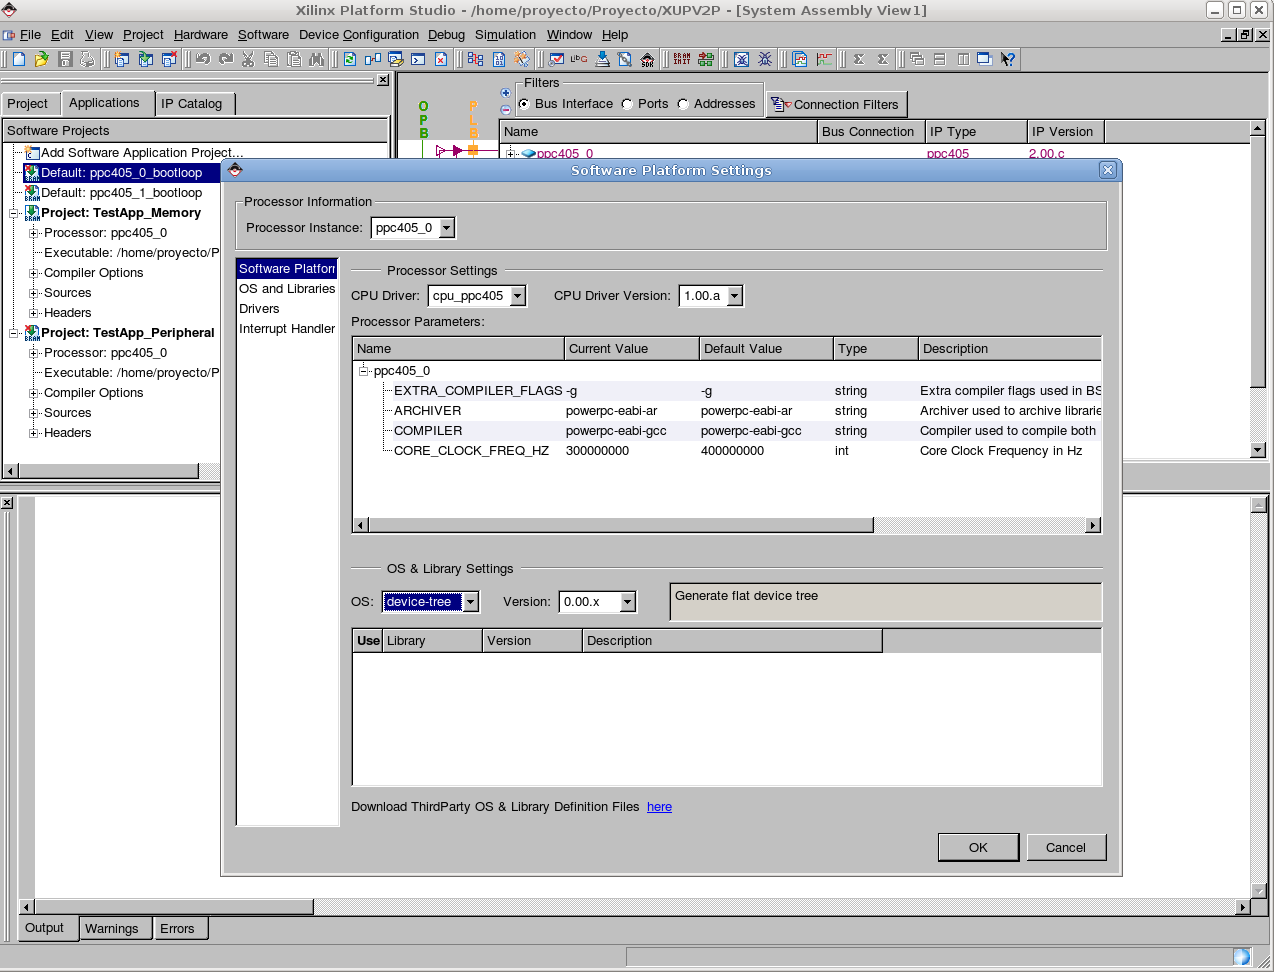
\includegraphics[scale=.25]{./figuras/devicetree.png}
  % capas.png: 607x522 pixel, 72dpi, 21.41x18.41 cm, bb=0 0 607 522
  \caption{Selección Device Tree}
  \label{devicetree}
  \end{figure}
  
  
\item Ajuste \emph{''console device''} a su UART. Actualizar \emph{``bootargs''}
para incluir \emph{console = ttyUL0, 115200}, \emph{figura}\ref{uart}.
  \begin{figure}[h!] 
  \centering
  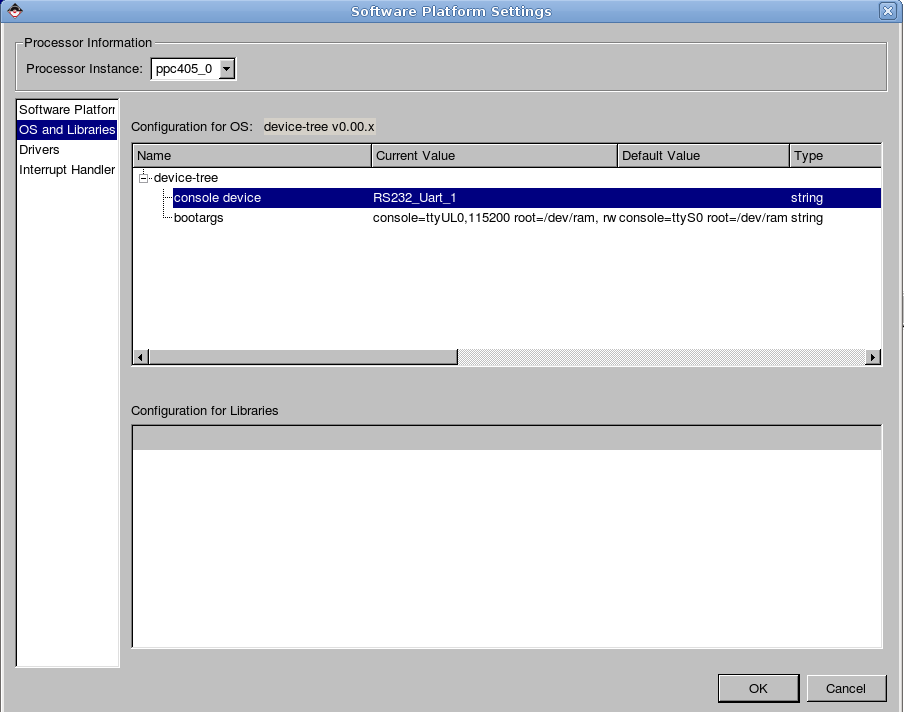
\includegraphics[scale=.25]{./figuras/uart.png}
  % capas.png: 607x522 pixel, 72dpi, 21.41x18.41 cm, bb=0 0 607 522
  \caption{BootArgs Kernel Command Line estática}
  \label{uart}
  \end{figure}
  
  
\item Generar el árbol de dispositivos, haga clic en el menú: \emph{``Software:
Generate Libraries and BSPs''}. El siguiente archivo se creará dentro de su
directorio del proyecto EDK: ./ppc405\_0/libsrc/device-tree/xilinx.dts. Este
archivo (xilinx.dts) se utilizará para ayudar a construir el kernel de Linux.

\end{enumerate}

El diseño final se puede apreciar en la figura\cite{system}, generada por el EDK

  \begin{figure}[h!] 
  \centering
  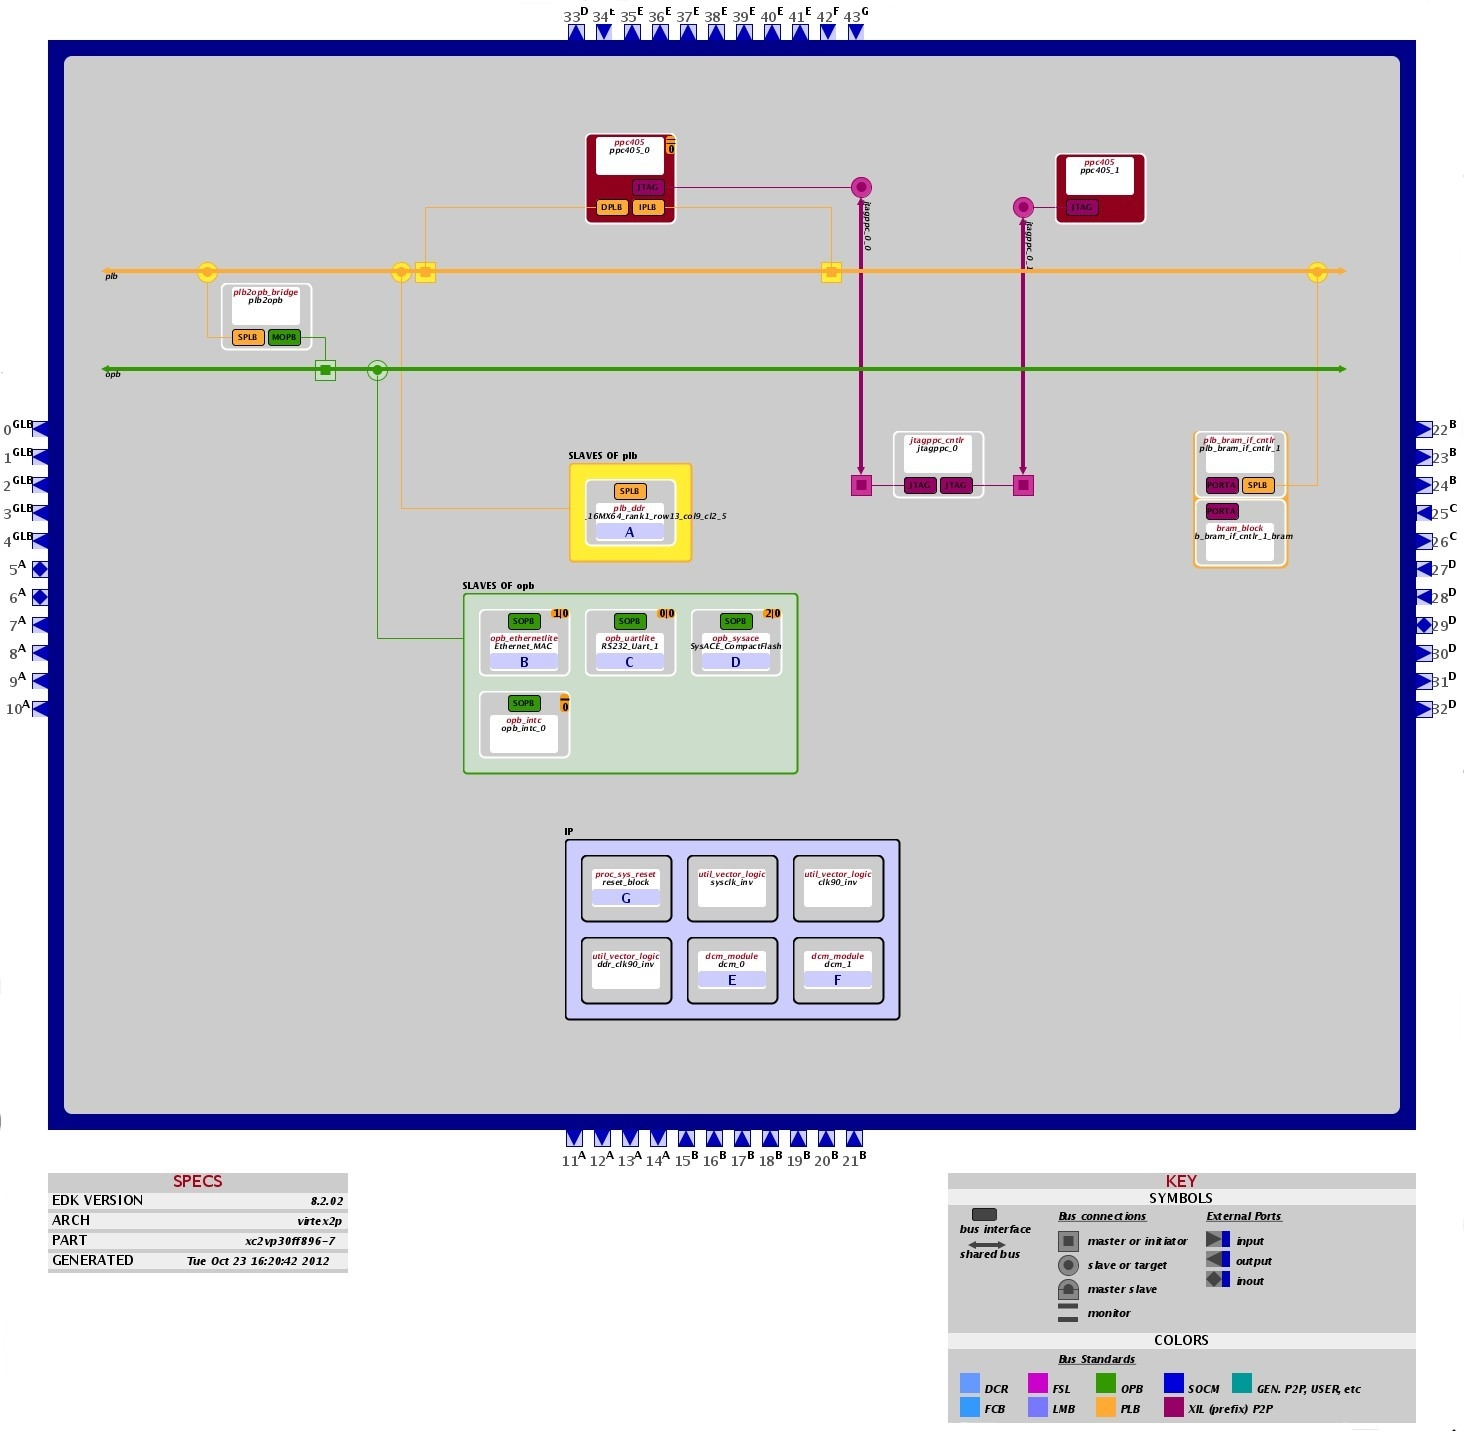
\includegraphics[scale=.40]{./figuras/system.jpg}
  % capas.png: 607x522 pixel, 72dpi, 21.41x18.41 cm, bb=0 0 607 522
  \caption{Diagrama de bloques del \emph{hardware} creado}
  \label{system}
  \end{figure}

\clearpage \newpage

\section{\emph{Device Tree File}}

El archivo xilinx.dts contine una descripción detallada del \emph{hardware}, un
mapa de memoria que permite acceder por DMA, el archivo ``xilinx.dts''
configurado se muestra en el \emph{Apéndice B}.


\chapter{Sistema Operativo}

\section{Introducción}

Un sistema de cómputo está compuesto de uno o más procesadores, una memoria
principal, discos, interfaces de red y otros dispositivos de entrada/salida. Al
ser un sistema complejo es necesario contar con una capa de \emph{software}
llamada sistema operativo, cuya labor es administrar todos los dispositivos y
proporcionar a los programas de usuario una interfaz sencilla para comunicarse
con el \emph{hardware}\cite{tanenbaum}.

Un sistema operativo puede definirse entonces como un conjunto de programas,
escrito en uno o más lenguajes de programación, utilizando diferentes
paradigmas de programación:

\begin{itemize}

 \item Lenguaje ensamblador dependiente de la arquitectura objetivo
 \item Lenguaje de mediano nivel no dependiente de la arquitectura
 \item Lenguajes interpretados o scripts, no dependiente de arquitectura
  objetivo
 
\end{itemize}

Su objetivo es proporcionar a los programas de usuario un
modelo de computadora mejor, más simple y encargarse de la administración de
todos los recursos.

\begin{figure}[ht]
 \centering
 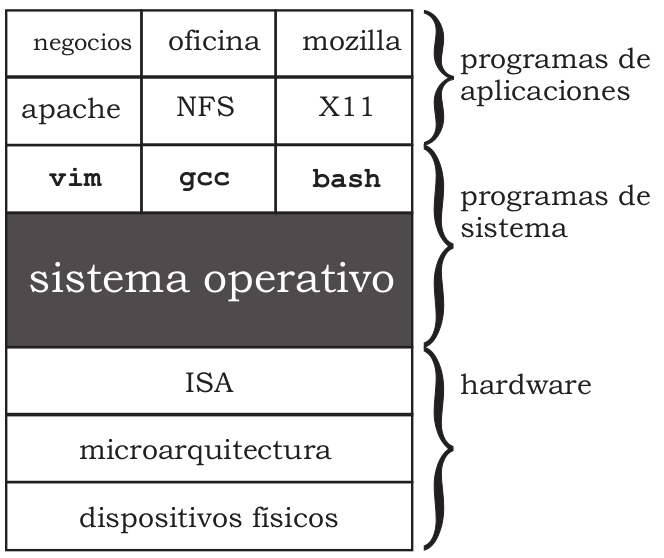
\includegraphics[scale=.50]{./figuras/capas.png}
 % capas.png: 607x522 pixel, 72dpi, 21.41x18.41 cm, bb=0 0 607 522
 \caption{Sistema de cómputo en capas}
 \label{Sistema de cómputo en capas}
\end{figure}


El sistema operativo tiene como misión administrar todos los elementos de un
sistema complejo, por tanto, el sistema operativo efectúa un reparto controlado
de los procesadores, memorias y dispositivos de entrada/salida, entre los
diversos programas que compiten por obtener estos recursos.

El sistema operativo (SO) permite lanzar aplicaciones a través de
procesos\footnote{Proceso, unidad de actividad que se caracteriza por la
ejecución de una secuencia de instrucciones, un estado actual, y un conjunto de
recursos del sistemas asociados\cite{tanenbaum}} o hilos\footnote{Hilo,  es la
unidad de procesamiento más pequeña que puede ser planificada por un sistema
operativo.} y vigilará que los recursos sean utilizados de forma equitativa
entre los procesos.

Para poder realizar estas tareas es necesario tener una jerarquía de ejecución,
esta jerarquía puede establecerse con:

\begin{itemize}

 \item Procesos con privilegos limitados
 \item Procesos con privilegos otorgados temporalmente
 \item Procesos con mayores privilegios
 
\end{itemize}

Para lograr que el sistema operativo logre su objetivo, es necesario que el
procesador tenga al menos dos modos de operación:

\begin{itemize}

 \item Modo \emph{kernel}, o supervisor, permite accesar a todo el
\emph{hardware} y
  permite la ejecución de cualquier instrucción.
 \item Modo usuario, o modo real, solo permite la ejecución de un conjunto
  reducido de instrucciones\cite{nsistemas}.
 
\end{itemize}

\section{Linux}


Linux tiene su origen en Unix, éste apareció en los años sesenta, desarrollado
por los investigadores Dennis Ritchie y Ken Thompson, de los Laboratorios
Telefónicos Bell.

Andrew Tanenbaum desarrolló un sistema operativo parecido a Unix (Minix)
para enseñar a sus alumnos el diseño de un sistema operativo. Debido al enfoque
docente de Minix, Tanenbaum nunca permitió que éste fuera modificado, ya que
podrían introducirse complicaciones en el sistema para sus alumnos.

Un estudiante finlandés llamado Linus Torvalds, constatando que no era posible
extender Minix, decidió escribir su propio sistema operativo compatible con
Unix.

En aquellos momentos el proyecto GNU (\emph{GNU's Not Unix}), que Richard
Stallman había iniciado hacía ya casi diez años, comprendía un sistema básico
casi completo. La excepción más importante era el \emph{kernel} o núcleo, que
controla el \emph{hardware}.

Torvalds decidió aprovechar el sistema GNU y completarlo con su propio núcleo,
que bautizó como Linux (\emph{Linux Is Not UniX}).

El \emph{kernel} es el componente central del sistema operativo. Su funciones
son principalmente administrar el \emph{hardware} de manera coherente y justa
mientras se le otorga un nivel de abstracción familiar, a través de las
APIs\footnote{ API acrónimonimo de \emph{Application Programming Interface}es el
conjunto de funciones y procedimientos que ofrece cierta biblioteca para ser
utilizado por otro software como una capa de abstracción.}, a las
aplicaciones de nivel de usuario.

Entre otras tareas relevantes de un sistema operativo, el \emph{kernel} de Linux
maneja dispositivos, administra los acceso de E/S, controla los procesos y
administra el uso compartido de memoria. Dentro del \emph{kernel}, la interfaz
de bajo nivel es específica para cada configuración de hardware, sobre la cual,
el \emph{kernel} ejecuta y provee control directo de los recursos hardware.

Típicamente, los servicios de bajo nivel manejan operaciones específicas de el
CPU, operaciones de memoria específicas a la arquitectura, y provee interfaces
básicas para dispositivos. Los capa de alto nivel provee abstracciones comunes a
todos los sistemas Unix, incluyendo procesos, archivos, sockets y señales. Este
nivel de abstracción se mantiene constante aunque difiera el hardware.

Entre estos dos niveles de abstracción, el \emph{kernel} necesita lo que se
denomina componentes de interpretación para comprender e interactuar con datos
estructurados provenientes de, o hacia ciertos dispositivos. Los diferentes
tipos de sistemas de archivos y los protocolos de red son ejemplos de fuentes de
datos estructurados. El \emph{kernel} necesita interpretarlos e interactuar a
fin de proveer acceso a los datos provenientes desde estas fuentes o hacia las
mismas.

Los servicios brindados por el \emph{kernel} no son soporte suficiente para
cargar y ejecutar las aplicaciones. Es necesario contar con librerías, éstas
proveen APIs familiares y abstracciones de servicios que interactúan con el
\emph{kernel} en nombre de las aplicaciones para obtener la funcionalidad
deseada.

La librería principal, utilizada en la mayoría de las aplicaciones Linux, es la
librería C GNU (\textbf{glibc}). Típicamente las librerías son enlazadas
dinámicamente en el momento en el que se ejecutan las aplicaciones. Esto es, no
son parte de las aplicaciones binarias, sino que se cargan dentro del espacio de
memoria de las aplicaciones durante el inicio de las mismas. Esto permite a
varias aplicaciones utilizar una misma instancia de una librería en vez de
realizar una copia en memoria por cada aplicación que se ejecuta.

Según lo expuesto anteriormente es lógico pensar la conveniencia de enlazar
dinámicamente las librerías, sin embargo, en los sistemas empotrados esto no es
del todo cierto. El motivo radica en que las aplicaciones no utilizan la
librería C en forma completa, sino que dependiendo de la aplicación puede
utilizar partes de la librería y no otras. De este modo, en algunas aplicaciones
parte de la librería se encuentra en la misma aplicación binaria. Este es el
fundamento por el cual es preferible utilizar un enlazamiento estático, sin
embargo nos encontramos con un inconveniente, para sistemas Linux empotrados la
librería \textbf{glibc} consume demasiados recursos de la memoria RAM del
sistema, por este motivo, reemplazar esta librería puede significar un ahorro de
espacio en memoria. Usualmente se la reemplaza por librerías alternativas
diseñadas para sistemas empotrados.

\subsection{El \emph{kernel} de Linux}

El \emph{kernel} Linux es distribuido bajo la licencia GNU GPL por lo que su
capacidad de evolución es una cualidad que posee desde su surgimiento, hecho por
el cual su desarrollo es muy activo, brindando soporte para cientos de
protocolos de red, decenas de arquitecturas de \emph{hardware} y por supuesto,
obteniendo un rendimiento eficiente y robusto\cite{emiliano}.

Una clasificación generalmente utilizada para clasificar a los sistemas
operativos tiene que ver con el modo de compartir el espacio de memoria. Se
diferencian tres tipos, de tiempo real, monolíticos y microkernel.
De forma resumida las características son las siguientes:

\begin{itemize}
 \item \emph{Realtime}, El espacio de direcciones es plano o lineal, no posee
protección de memoria entre las aplicaciones y el \emph{kernel}, es decir, el
núcleo del \emph{kernel}, el subsitema del \emph{kernel} y las aplicaciones
comparten el mismo espacio de memoria. Se denominan \emph{Realtime} debido a que
no hay sobrecarga por llamadas al sistema, pasaje de mensajes o copia de datos.

   \item Monolítico, está diferenciado el espacio de memoria de usuario y
\emph{kernel}. Las aplicaciones que operan en el espacio de usuario lo hacen
sobre direcciones de memoria virtuales por lo tanto no pueden corromper la
memoria de otras aplicaciones o del \emph{kernel}. Sin embargo, los componentes 
del \emph{kernel} comparten el mismo espacio de direcciones y por ende, un
\emph{drive} o módulo mal programado puede causar la inestabilidad del sistema.
La mayoría de os sistemas operativos Unix son de este tipo.                    
            

  \item Microkernel,  hace uso de un pequeño SO que provee los servicios básicos
y el resto del \emph{kernel} se ejecuta como aplicaciones. La clave del
microkernel surge a partir de un esquema robusto de paso de mensajes.

\end{itemize}

Cuando un programa es ejecutado en modo usuario este no puede acceder
directamente a programas o estructuras de datos del \emph{kernel}, sin embargo,
cuando el mismo se ejecuta en modo \emph{kernel} estas restricciones no existen.


\subsection{Sistema de archivos}

El sistema de archivos es el encargado de realizar la organización y
almacenamiento de los archivos en los diferentes dispositivos disponibles en el
sistema. En función de las características del dispositivo de almacenamiento y
del tipo de información que se va a guardar es preferible utilizar un sistema de
archivos u otro.

Linux da soporte a varios sitemas de archivos, dentro de los más utilizados se
encuentran ext2, ext3, etc. Estos sistemas de archivos son manejados
por una capa denominada Sistema de Archivos Virtual (VFS\footnote{VFS, es una
capa de abstracción encima de un sistema de archivos más concreto. El propósito
de un VFS es permitir que las aplicaciones cliente tengan acceso a diversos
tipos de sistemas de archivos concretos de una manera uniforme. Puede ser
utilizada para tender un puente sobre las diferencias en los sistemas de
archivos de Windows, de Mac OS y Unix, de modo que las aplicaciones pudieran
tener acceso a archivos en los sistemas de archivos locales de esos tipos sin
tener que saber a qué tipo de sistema de archivos están teniendo acceso.}). Esta
capa de abstracción provee una visión consistente de los datos almacenados en
diferentes dispositivos del sistema. Esta visión es lograda separando el nivel
de usuario de los sistemas de archivos, utilizando llamadas estándar al
sistema, permitiendo sistemas de archivos lógicos sobre cualquier dispositivo
físico. Por lo tanto esta capa abstrae los detalles físico del dispositivo
permitiendo un acceso a los mismos a través de archivos de una maner
consistente.

Por debajo de esta capa VFS, el \emph{kernel} interactúa con dispositivos de E/S
a través de controladores de dispositivos. Estos controladores se encuentran
incluidos en el \emph{kernel} y consisten en estructuras de datos y funciones
que controlan uno o más dispositivos como discos rígidos, teclados, mouses,
monitores, interfaces de red, dispositivos SCSI.

Uno de los propósitos fundamentales de los controladores de dispositivos es
aislar los programas de usuario del acceso a estructuras de datos críticas del
\emph{kernel} y dispositivos de \emph{hardware}. Además, un controlador de
dispositivo oculta al usuario la complejidad y variabilidad de un dispositivo
\emph{hardware}. Por ejemplo, un programa que quiere escribir datos en un disco
rígido no tiene en cuenta si el mismo posee sectores de 512 bytes o 1024 bytes.
El usuario simplemente abre el archivo y realiza el comando de escritura. El
controlador manejará los detalles y aislará al usuario de las complejidades y
riesgos de programar directamente sobre el dispositivo de \emph{hardware}. Estos
controladores proveen la representación de los dispositivos a través de
archivos, en GNU/Linux y sistemas operativos Unix todo \emph{hardware} es
representado por un archivo.

Linux posee la capacidad de agregar y quitar componentes del \emph{kernel} en
tiempo de ejecución. Como hemos descrito anteriormente, el \emph{kernel} Linux
posee una estructura de \emph{kernel} monolítico, con una interfaz para agregar
y quitar módulos de controladores de dispositivos dinámicamente luego del
arranque del mismo. Esta característica no solo agrega flexibilidad al usuario,
sino que además, en sistemas empotrados adquiere una especial importancia debido
a su capacidad de actualización y adaptación a dispositivos de E/S
nuevos\cite{understanding}.

Todo dispositivo, ya sea que se encuentre en un sistema empotrado o una PC de
escritorio, necesita al menos un sistema de archivos. La principales razones de
esto son:

\begin{itemize}
 \item Las aplicaciones poseen programas separados, independientes por ende
necesitan espacio de almacenamiento en un sistema de archivos.
 \item Los dispositivos de bajo nivel también son accedidos mediante archivos.
\end{itemize}

\section{\emph{Embedded Linux}}

Linux empotrado, del inglés: \emph{Embedded Linux} se refiere al uso de un
sistema operativo basado en Linux en un sistema empotrado, como por ejemplo
teléfonos móviles, robots, servidores, dispositivos electrónicos y aplicaciones
industriales con microcontroladores y microprocesadores\cite{embedded}.

Para implementar un sistema Linux empotrado en un dispositivo de
\emph{hardware}, se debe conocer en términos generales la arquitectura del
mismo, es decir, el tipo de micro-procesador que posee, la cantidad de memoria,
los buses que soporta, los componentes que posee la tarjeta de desarrollo,
etc. Esta información es de vital importancia, ya que al preparar el sistema
Linux que se ejecutará en el dispositivo, se debe compilar con soporte
para esas características. La tarea de construir un sistema operativo
basado en Linux que se ejecute en este dispositivo objetivo se debe
realizar mediante compilación cruzada.

\subsection{¿Por qué \emph{Embedded Linux}?}
 
\subsubsection{Independiencia de Proveedores}

Selecionar un sistema operativo propietario para la construcción de este
proyecto podría limtar la vida útil del mismo, la falta de  soporte por parte
del proveedor resultaría en mayor tiempo de desarrollo, \emph{Embedded Linux}
es un sistema operativo independiente el cual comparte muchas caraceristícas
con sistemas operativos propietarios como puden ser el \emph{kernel},
librerias, utilidades básicas, etc.

\subsubsection{Variedad de \emph{hardware} soportado}

Debido al crecimiento exponencial de componentes para sistemas embebidos las
dificultades para dar soporte a todos estos componentes a  aumentado
considerablemente,\emph{Embedded Linux} soporta multiples arquitecturas y
dispositivos de entrada y salida, además es aceptado en univeridades como una
herramienta de desarrollo e investigación lo que ayuda  a mantener una gran
variedad de \emph{hardware} soportado por el \emph{kernel}.

\subsubsection{Bajo Costo}

\emph{Embedded Linux} conlleva bajos costos en su desarrollo , capacitación y
mantenimiento, además todas las herramientas como compiladores, \emph{linkers},
librerias, \emph{shells} pueden ser descargadas a través de internet de forma
libre,

\subsection{\emph{Open Source}}

Una de las principales razones por las que Linux es tan popular es que es de
código abierto, Linux tiene  ventajas del \emph{Open
Source}\cite{raghavan2005embedded} como:
\begin{itemize}
 \item Hay miles de desarrolladores contibuyendo a la mejora continua del
 \emph{kernel} de Linux y otras aplicaciones.
 \item Asegura un soprte global durante el proceso de desarrollo.
 \item Amplia disponibilidad de código  y controladores de dispositivos de
 \emph{hadware}.
 \item Las aplicaciones y utilidades integradas con Linux tienen una naturaleza
\emph{Open Source}, teniendo todos los beneficios antes mencionados. 
\end{itemize}
















\chapter{Compilación del \emph{kernel}}

\section{Introducción}

La compilación se refiere al proceso de traducción de un lenguaje de alto nivel
a otro funcionalmente equivalente, expresado en lenguaje ensamblador de una
arquitectura específica\cite{compilacion}. Durante este capítulo se explica la
técnica para crear una toolchain que genere binarios para la plataforma PPC405.


\section{El proceso de compilación}

El proceso de compilación es el proceso por el cual se traducen las
instrucciones escritas en un determinado lenguaje de programación a lenguaje
máquina. Además de un traductor, se pueden necesitar otros programas para crear
un programa objeto ejecutable. Un programa fuente se puede dividir en módulos
almacenados en archivos distintos. La tarea de reunir el programa fuente a
menudo se confía a un programa distinto, llamado preprocesador. El preprocesador
también puede expandir abreviaturas, llamadas a macros, a proposiciones del
lenguaje fuente.

\begin{figure}[ht]
 \centering
 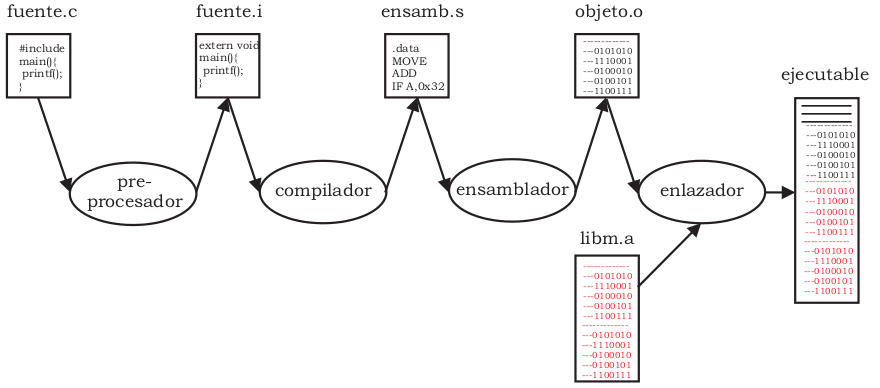
\includegraphics[scale=.45]{./figuras/compilacion.png}
 % capas.png: 607x522 pixel, 72dpi, 21.41x18.41 cm, bb=0 0 607 522
 \caption{El proceso de compilación}
 \label{El proceso de compilación}
\end{figure}

Este proceso se compone internamente de varias etapas mostradas a continuación:

\begin{itemize}
 \item Análisis léxico, se encarga de la reducción del texto del programa en
  \emph{tokens}:
    \begin{itemize}
      \item identificadores
      \item separadores operadores
      \item constantes
    \end{itemize}

  \item Análisis sintáctico, se encarga del análisis de símbolos para
  reconocer la estructura de programa:
  \begin{itemize}
   \item indentificador = expresión
   \item indentificador + constante
  \end{itemize}
  
  \item Análisis semántico, realiza la asociación de identificadores con zonas
  de memoria y la asociación de tipos de datos.

  \item Generación de código, Asocia las sentencias con secuencias de
  instrucciones.
  
  \item Optimización de código, consiste en mejorar el código intermedio, de
  modo que resulte un código máquina más rápido de ejecutar.

\end{itemize}

\section{Compilación cruzada}

Si un compilador es capaz de compilar un programa para otra arquitectura en la
cual se está ejecutando, se dice que es un compilador cruzado. En este proceso
se identifica al equipo que realiza la compilación mediante el término
\emph{Host} o Huesped y al dispositivo que ejecuta el software, como sistema
\emph{Target} u Objetivo\cite{building}.

\subsection{Sistema huesped}

La implementación de un entorno de compilación cruzada nos brinda la
posibilidad de aprovechar los recursos que disponemos en una PC. Esta tarea se
ha llevado a cabo sobre una PC de escritorio con las siguientes características:

\begin{itemize}
 \item 2 Procesadores Intel(R) Core(TM) 2 Duo 3.16GHz
 \item Memoria 1.9 GiB
 \item Sistema Operativo Debian GNU/Linux 6.0.5 (squeeze)
 \item Kernel Linux 2.6.32-5-amd64
\end{itemize}


\subsection{Sistema objetivo}

El sistema objetivo es la tarjeta de desarrollo XUPV2, dentro de ella se
cuenta con un FPGA Xilinx Virtex-II Pro 50 con las siguientes características:

  \begin{itemize}
  \item FPGA Virtex-2 Pro XC2VP30  con 30,816 celdas lógicas, 136 18-bit
multiplicadores,
  2,448Kb bloques de RAM y 2 Procesadores PowerPC.
  \item DDR SDRAM DIMM de hasta  2Gbytes de RAM
  \item Puerto Ethernet 10/100
  \item Puerto USB2 
  \item Lector de tarjetas Compact Flash
  \item Puerto de video XSGA
  \item Audio Codec
  \item Puertos SATA, S/2 y RS-232
  \end{itemize}
   
\begin{figure}[ht]
 \centering
 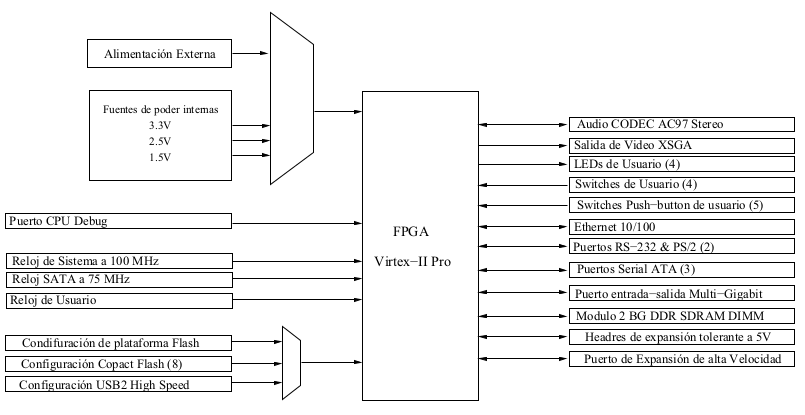
\includegraphics[scale=.50]{./figuras/virtex.png}
 % capas.png: 607x522 pixel, 72dpi, 21.41x18.41 cm, bb=0 0 607 522
 \caption{Diagrama a bloques de la tarjeta Virtex-II Pro 50}
 \label{Diagrama a bloques de la tarjeta Virtex-II Pro 50}
\end{figure}

Estas características proporcionan un gran número de posibilidades para
el desarrollo de aplicaciones y, puesto que existen hoy en día herramientas de
software que ayudan a la programación, compilación, sıntesis, simulación y
depuración tanto de hardware como de software, se obtiene una alta flexibilidad
de desarrollo, permitiendo a los usuarios centrarse en el diseño y tomando la
responsabilidad de dicho diseño para obtener el máximo provecho de los
recursos\cite{alvarado}.



\subsection{GNU \emph{toolchain}}

GNU toolchain es un término que agrupa a una serie de proyectos que contienen
las herramientas de programación producidas por el proyecto GNU. Estos proyectos
forman un sistema integrado que es usado para programar tanto aplicaciones como
sistemas operativos.

El GNU toolchain es un componente vital en el desarrollo del núcleo Linux, el
desarrollo del BSD y software para sistemas empotrados.

Cualquier compilador requere librerías de soporte (como
\emph{libc}\footnote{\emph{libc}, es una recopilación de ficheros cabecera y
bibliotecas con rutinas, estandarizadas por un comité de la Organización
Internacional para la Estandarización (ISO), }) además de bianrios
(ensambladores y \emph{linkers}), una \emph{toolchain} requiere estos mismos
componentes también, una \emph{toolchain} tiene los componentes enlistados a
continuación:
\begin{itemize}
 \item \emph{Binutils}, es un conjunto de programas necesarios para el enlace,
 ensable y compilación.
 \item Compilador GNU, compilador básico de lenguaje C, usado para obtener un
código objeto.
 \item Librerías C GNU, esta librería implementa llamadas al sistema, cualquier
aplicación desarrollada necesita ser ligada a esta librería base.
\end{itemize}

\section{Construyendo una \emph{toolchain}}

Los pasos para construir una \emph{toolchain} se citan a continuación:
\begin{enumerate}
 \item Decidir el sistema objetivo.
 \item Decidir versiones de \emph{kernel/gcc/glibc/binutlis}.
 \item Compilar \emph{binutlis}.
 \item Obtener los \emph{kernel headers} para la plataforma objetivo.
 \item Compilar una versión minima de \emph{gcc}.
 \item Construir \emph{glibc}.
 \item Recompilar \emph{gcc}.
\end{enumerate}

\section{Fuentes del \emph{kernel}}

El \emph{kernel} de Linux puede obtenerse desde muchos repositorios, sin
embargo la fuente principal para descarga se encuentra disponible en
\emph{http://www.kernel.org/} en donde se puede descargar la versión actual
disponible así como también versiones anteriores.

\subsection{linux-xlnx}

\emph{linux-xlnx} es una rama del \emph{kernel} mantenida por la empresa
Xilinx, la cual tiene actualizados una serie de parches y ofrece soporte para
una amplia gama de periféricos presentes en sus tarjetas de desarrollo.

Para obtener este \emph{kernel} se usa el siguiente comando:

\begin{verbatim}
 Proyecto@debian$ git clone git://git.xilinx.com/linux-2.6-xlnx.git
\end{verbatim}



\section{Configuración del \emph{kernel}}


El \emph{kernel} de Linux debe de ser compilado con la ayuda de una
\emph{toolchain} que nos permita alcanzar la arquitectura objetivo
(\emph{PowerPC 405}).

La \emph{toolchain} usada en este proyecto para compilar el \emph{kernel} esta
descrita en el protecto terminal \emph{``Plataforma para la ejecución paralela
en un sistema embebido basado en FPGA''}\cite{Beto}, para cargar las variables
de entorno necesarias para el uso de la \emph{toolchain} se ejecuta el siguiente
\emph{script}:


\begin{verbatim}
 Proyecto@debian$ source
/home/Proyecto/Crosstool/powerpc-405-linux-uclibc/loadembenv.sh
\end{verbatim}


\lstinputlisting[caption=Archivo loadembenv.sh,language=sh]
{./code/loadembenv.sh}


El archivo ``.config'' se usa para controlar las partes del \emph{kernel} que
serán incluidas, se debe de ser muy cuidadoso con la configuración del
\emph{kernel}, si se selecciona algún componente de manera errónea la
compilación puede fallar.

No es  recomendable editar el archivo ``.config'' directamente, existen
programas que ayudan a la configuración de este archivo como
\emph{makmenuconfig} y \emph{make xconfig}, el archivo ``.config''
configurado se muestra en el \emph{Apéndice B}.

Una vez que se configura el \emph{kernel}, se procede a la compilación con el
siguiente comando:
\begin{verbatim}
  Proyecto@debian$ make simpleImage.virtex405-nombre_del_proyecto
\end{verbatim}


\section{system.ace}


\emph{System Advanced Configuration Environment} (System ACE) es una tecnología
que proporciona un ahorro sustancial en el desarrollo y el costo por bit de
almacenamiento.

\begin{figure}[ht]
 \centering
 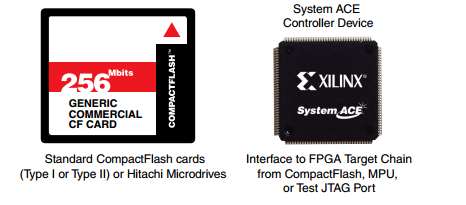
\includegraphics[scale=.70]{./figuras/SystemACE.png}
 % capas.png: 607x522 pixel, 72dpi, 21.41x18.41 cm, bb=0 0 607 522
 \caption{SystemACE}
 \label{SystemACE}
\end{figure}

La tarjeta de desarrollo \emph{XUPV2P} puede hacer la carga por
\emph{system.ace} de los archivos ELF (\emph{Executable and Linkable Format}),
el archivo ``simpleImage.virtex405-micheangeloEXT2.elf'' generado en la
compilación del \emph{kernel} se encuentra en la ruta
\emph``/arch/powerpc/boot/'' del directorio del \emph{kernel}.

Para generar el ``systme.ace'' se utiliza el siguiente archivo de configuración:

\lstinputlisting[caption=Archivo xupGenaceEXT2.opt,language=C]{
./code/xupGenaceEXT2.opt}

Y se procede con el comando:
\begin{verbatim}
 Proyecto@debian$ xmd -tcl genace.tcl -opt xupGenaceEXT2.opt
\end{verbatim}

El comando anterior genera el archivo ``system.ace'' el cual contiene la
configuración del \emph{kernel} que funcionará en la tarjeta, este archivo
junto con la configuración obtenida al diseñar el \emph{hardware} en el archivo
``xilinx.dts'' determinará la forma de arranque de nuestro sistema embebido.







\chapter{\emph{Root File System}}


\section{Introducción}

El sistema de archivos \emph{root file system} se encuentra localizado en la
misma partición en donde esta el directoio \emph{root} y es el sistema de
archivos en donde cualquier otro sistema de archivos serán montados.

Una partición es una seción lógica independiente de una unidad de
almacenamiento, un sistema de archivos es una jerarquia de directorios
utilizada para organizar los archivos de un istema de cómputo, en Linux, se
comienza con el directoio \emph{root}, el cual contiene una serie de
subdirectorios,cada uno  a su vez contiene directorios adicionales, etc. 


El contenido exacto del \emph{root file system}  puede variar en cada sistema
de cómputo, pero puede inclur los archivos necesarios para el arranque del
sistema, asi como también los archivos necesarios para montar otros sistemas de
archivos. El contenido del directorio \emph{root} junto con una cantidad mínima
de directorios incluyen los directorios \emph{/boot, /dev, /etc, /bin, /sbin}.

El  \emph{root file system} es generalmente pequeño, lo que ayuda a evitar que
el sistema de archivos sea corrupto, Un sistema de archivos corrupto puede
evitar el arranque del sistema\cite{rootfs}.

\section{\emph{BuildRoot}}

\emph{BuildRoot} es una serie de archivos de configuración que permiten la
creacion de un entorno de compilación cruzada mediante el uso de una
\emph{toolchain}, \emph{BuildRoot} es capaz de construir un sitema de archivos
(\emph{root file system}) o una imagen de Linux, ambas funciones pueden ser
usadas de forma independiente.

Además \emph{BuildRoot} proveé una inferstructura que permite reproducir el
proceso de desarrollo de un \emph{root file system}, esto es particularmente
útil cuando es necesario depurar, actualizar o agregar parches a un sistema de
archivos creado anteriormente\cite{buildroot}.

\emph{BuildRoot} se pude obtener suando Git\footnote{Git, es un software de
control de versiones diseñado por Linus Torvalds, pensando en la eficiencia y la
confiabilidad del mantenimiento de versiones de aplicaciones cuando estas tienen
un gran número de archivos de código fuente.} a travéz del siguiente comando :
\begin{verbatim}
  Proyecto@debian: git clone git://git.buildroot.net/buildroot
\end{verbatim}

\subsection{Configuración y uso general}

\emph{BuildRoot} tiene un configuración similar a la del \emph{kernel} de
Linux, por lo que se puede generar la configuración desde un asistente
ejecutando:
\begin{verbatim}
  Proyecto@debian: make menuconfig
\end{verbatim}

El archivo de configuración ``.config'' de \emph{BuildRoot}  se muestra en el
\emph{Apéndice B}.

Una vez que se han configurado todos los componentes que tendrá el \emph{root
file system} se procede a compilar el sistema de archivos con el comando:
\begin{verbatim}
  Proyecto@debian: make 
\end{verbatim}

Este comando realizará los siguientes pasos:
\begin{itemize}
 \item Descargara las fuentes necesarias.
 \item Configurará, instalará o importará la \emph{toolchain} que usara para
compilar los paquetes seleccionados en la configuración.
 \item Constriurá e instalará los paquetes objetivo.
 \item Creará el sistema de archivos en el formato seleccionado (\emph{ext2}
para este protecto).
\end{itemize}

La salida generada por \emph{BuildRoot} será almacenada en el directorio
\emph{``output/''}, este directorio contiene a su vez los siguientes
directorios:
\begin{itemize}
 \item \emph{``images/''}, en donde se encuentran todas las las imagenes 
guardadas
(kernel, sistema de archivos).
 \item \emph{``build/''}, contiene todos los compenentes que serán construidos.
 \item \emph{``staging/''}, contiene una jerarquía similar  ala que se generará
 el \emph{root file system}.
 \item \emph{``target/''}, contiene el \emph{root file system} completo.
 \item \emph{``host/''}, contiene las herramientas necesarias para la
compilación del \emph{root file system} desde el sistema huesped.
 \item \emph{``toolchain/''}, contiene los componentes de la \emph{toolchain}.
\end{itemize}




\chapter{Primer entorno generado}

\section{Introducción}

Una vez que se ha realizado la compilación del \emph{kernel} y se ha creado el
\emph{root file system} se cuenta con los recursos necesarios para realizar
pruebas sobre la tarjeta de desarrollo \emph{XUPV2P}.

\section{Formato de la \emph{compact flash}}

La \emph{compact flash}  deberá de tener  dos particiones para su correcto
funcionamiento en este proyecto, la primera partición será en formato FAT16 y en
donde estará localizado el archivo ``system.ace'', la segunda en formato
\emph{ext2} en donde se encontrará el \emph{root file system}.

La primera partición deberá de ser formateada bajo un sistema operativo
\emph{Windows} con la herramienta \emph{mkdosfs}\footnote{\emph{mkdosfs} es el
comando para crear un sistema MS-DOS FAT32 archivos bajo Linux, y como tal
similar en uso a mkfs.} con el siguiente comando:

\begin{verbatim}
 mkdosfs -s 64 -F 16 -R 1 F:
\end{verbatim}

Esta partición contendra el \emph{root file system} genrado anteriormente.

A la segunda partición se le asignará un formato \emph{ext2}, en esta partición
deberá de ser copiado el \emph{system.ace}.

\section{Modificación del \emph{device tree}}

Para poder juntar el \emph{kernel} con el \emph{root file system} generado será
necesario hacer modificaciones en el archivo ``xilinx.dts''  modificando la
siguiente linea  :

\begin{lstlisting}[caption=Archivo ``xilinx.dts'' ]
		bootargs = "console=ttyUL0,115200 root=/dev/ram, rw";
\end{lstlisting}
por :
\begin{lstlisting}[caption=``xilinx.dts'' ]
		bootargs = "console=ttyUL0,115200 root=/dev/xs`2 rw ip=dhcp";
\end{lstlisting}

Esta nueva configuración  permite al sistema montar el \emph{root file system}
desde la tarjeta \emph{compact flash}, además solicita a un servidor dhcp una
dirección IP. Debido a las modificaciones hechas al archivo ``xilinx.dts'' es
necesario recompilar el kernel y generar de nueva cuenta el
archivo ``system.ace''.


\section{Configuración de terminal}

Una vez que se han realizado las operaciones anteriores y se han copiado los 
archivos a la tarjeta \emph{compact flash} se proceden a realizar pruebas en
la tarjeta de desarrollo, para ello es necesario configurar una consola remota,
en este proyecto se hizo uso de \emph{Minicom}\footnote{Minicom es un programa
de módem basado en texto y emulación de terminal para sistemas operativos
\emph{UNIX}, originalmente escrito por Miquel Van Smoorenburg, y modelado de
acuerdo con el popular programa de MS-DOS Telix.}, la configuración se realiza
con los siguientes comandos:

\begin{verbatim}
  Proyecto@debian$sudo minicom -s
              +-----[configuration]------+
            | Filenames and paths      |
            | File transfer protocols  |
            | Serial port setup        |
            | Modem and dialing        |
            | Screen and keyboard      |
            | Save setup as dfl        |
            | Save setup as..          |
            | Exit                     |
            | Exit from Minicom        |
            +--------------------------+
    +----------------------------------------------------------+
    | A -    Serial Device      : /dev/USB0                    |
    | B - Lockfile Location     : /var/lock                    |
    | C -   Callin Program      :                              |
    | D -  Callout Program      :                              |
    | E -    Bps/Par/Bits       : 115200 8N1                   |
    | F - Hardware Flow Control : Yes                          |
    | G - Software Flow Control : No                           |
    |                                                          |
    |    Change which setting?                                 |
    +----------------------------------------------------------+
    
\end{verbatim}

\section{Arranque del sistema}

En este punto se tiene configurada la terminal para poder acceder a la tarjeta
de desarrollo, una vez que se coloca la \emph{compact flash} se enciende el
sistema el cual genera una salida mostrada en el el \emph{Apéndice B}.

Durante el arranque del sistema se generan llaves para la conexión via remota,
esto se puede observar de la siguente manera:

\begin{verbatim}
 Generating RSA Key...
Generating public/private rsa1 key pair.
Your identification has been saved in /etc/ssh_host_key.
Your public key has been saved in /etc/ssh_host_key.pub.
The key fingerprint is:
d7:2c:95:b1:0d:21:b1:db:2c:4d:ae:55:c9:14:77:5c 
The key's randomart image is:
+--[RSA1 2048]----+
|          o.+.ooE|
|           o O oo|
|          . = =  |
|           @ .   |
|        S = O    |
|         . =     |
|          .      |
|                 |
|                 |
+-----------------+
\end{verbatim}

Una vez que se han generado la llaves y el sistema a arrancado se inicia una
sesión como administrador del sistema:

\begin{verbatim}
 XUPV2P-MicheAngelo login: root
[root@XUPV2P-MicheAngelo /]#
\end{verbatim}

Como adminustrador del sistema se verifican los recursos disponibles:

\begin{verbatim}
[root@XUPV2P-MicheAngelo ~]# uname -a
Linux XUPV2P-MicheAngelo 3.2.0 
#6 Wed Oct 17 16:16:35 CDT 2012 ppc GNU/Linux
[root@XUPV2P-MicheAngelo ~]# cat /proc/cpuinfo 
processor       : 0
cpu             : Virtex-II Pro
clock           : 300.000000MHz
revision        : 8.160 (pvr 2001 08a0)
bogoppc        : 600.00
timebase        : 300000000
platform        : Xilinx Virtex
model           : testing
Memory          : 256 MB
[root@XUPV2P-MicheAngelo ~]# cat /proc/meminfo 
MemTotal:         252820 kB
MemFree:          242268 kB
Buffers:             240 kB
Cached:             6376 kB
SwapCached:            0 kB
Active:             4308 kB
Inactive:           3116 kB
Active(anon):        824 kB
Inactive(anon):        8 kB
Active(file):       3484 kB
Inactive(file):     3108 kB
Unevictable:           0 kB
Mlocked:               0 kB
HighTotal:             0 kB
HighFree:              0 kB
LowTotal:         252820 kB
LowFree:          242268 kB
SwapTotal:             0 kB
SwapFree:              0 kB
Dirty:                16 kB
Writeback:             0 kB
AnonPages:           816 kB
Mapped:             2012 kB
Shmem:                24 kB
Slab:               3584 kB
SReclaimable:        780 kB
SUnreclaim:         2804 kB
KernelStack:         216 kB
PageTables:          128 kB
NFS_Unstable:          0 kB
Bounce:                0 kB
WritebackTmp:          0 kB
CommitLimit:       62408 kB
Committed_AS:       2264 kB
VmallocTotal:     890880 kB
VmallocUsed:         160 kB
VmallocChunk:     890684 kB
[root@XUPV2P-MicheAngelo ~]#   
\end{verbatim}

\section{Compilación cruzada para Virtex-II Pro}

Gracias a \emph{buildroot} se cuenta ya con un entorno de compilación cruzada
capaz de generar archivos binarios que pueden ejecutarse desde la  tarjeta de
desarrollo de forma nativa, para poder compilar una aplicación para el entorno
generado es necesario configurar un par de variables de entorno :

\begin{lstlisting}[caption=Variables de entorno para compilación cruzada',]
export TOOLCHAIN_PPC=/opt/toolchains-ppc/buildroot-2011.05
export PATH=$TOOLCHAIN_PPC/output/host/usr/bin:$PATH
 
export AR=$TOOLCHAIN_PPC/output/host/usr/bin/ppc-linux-ar
export AS=$TOOLCHAIN_PPC/output/host/usr/bin/ppc-linux-as
export CC=$TOOLCHAIN_PPC/output/host/usr/bin/ppc-linux-gcc
export CPP=$TOOLCHAIN_PPC/output/host/usr/bin/ppc-linux-cpp
export CXX=$TOOLCHAIN_PPC/output/host/usr/bin/ppc-linux-g++
export LD=$TOOLCHAIN_PPC/output/host/usr/bin/ppc-linux-ld
export GCC=$TOOLCHAIN_PPC/output/host/usr/bin/ppc-linux-gcc
export NM=$TOOLCHAIN_PPC/output/host/usr/bin/ppc-linux-nm
\end{lstlisting}

Se procede a escribir una aplicación para probar la compilación cruzada:
\lstinputlisting[caption= Holavirtex.c,language=C]{./code/Holavirtex.c}

Ahora es  posible realizar la compilación cruzada desde el sistema huesped (x86)
hasta el sistema objetivo \emph{PPC045}, a través del binario
\emph{ppc-linux-gcc}, además vamos a agregar el \emph{flag static} para crear un
binario estático.
\begin{verbatim}
 ppc-linux-gcc /tmp/helloworld.c -static -s -o /tmp/helloworld-ppc
\end{verbatim}

El ejecutable generado debe de ser copiado y ejecutado en la tarjeta de
desarrollo como se indica :

\begin{verbatim}
 Proyecto@debian$ scp /tmp/helloworld-ppc root@192.168.1.1:/
\end{verbatim}

Y desde \emph{minicom} se ejecuta la aplicación:

\begin{verbatim}
 [root@XUPV2P-MicheAngelo ~]#  ./helloworld-ppc
 Hola Virtex!
 Hola Virtex!
 Hola Virtex!
 Hola Virtex!
 Hola Virtex!
 [root@XUPV2P-MicheAngelo ~]#
\end{verbatim}




\chapter{Virus}

\section{Introducción}

Un virus, es un \emph{software} o un fragmento de \emph{software} introducido
subrepticiamente en la memoria de una computadora que, al activarse, destruye
total o parcialmente la información almacenada, esta diseñado para propagarse de
un equipo a otro e interferir en el funcionamiendo de los mismos\cite{lehtinen}.

Los virus comienzan a ejecutarse cuando inicia el programa que lo contiene. El
virus puede reproducirse asi mismo, en mucho casos los virus necesitan
reproducirse para poder ser una verdadera amenaza. Los virus pueden
reporducirse de forma inmediata o hasta que algún evento que propicie su
reproducción. Por ejemplo, en una fecha exacta ( como con el famoso virus
\emph{Friday the 13th\footnote{\emph{Friday the 13th}, fue un virus
que consistía en borrar cada programa que fuera ejecutado en una
computadora, cada dia viernes 13.}})

Recientemente  fue necesario que un usuario actuvará un virus ejecutando un
programa corrupto, el cual pudo ser abierto desde algun archivo oculto en un
correo electrónico. La mayoria de los lectores de correo electrónico actuales
tienen la posibilidad de incluir archivos adjuntos dentro del correo
electrónico, por lo que atacantes buscan incluir \emph{malware} en estos
archivos.

La información es hoy la materia prima de las organizaciones. Tener información
ayuda a tomar decisiones con seguridad y rapidez. Por tanto, proteger la
información en todo momento y permitir el acceso a ella sólo para las personas
que la necesiten y que, además, sea fiable, es un tema fundamental.

Los virus inform\'aticos son hoy una realidad reconocida por las empresas,
quienes saben que es un problema que mina su productividad, ya que sus
computadoras est\'an constantemente expuestas a vulnerabilidades de sus sistemas
de seguridad.

Actualmente los FPGAs son dispositivos que permiten la implementaci\'on de
complejos sistemas de seguridad basados en \emph{hardware} o \emph{software}
ofreciendo a los desarrolladores una alta gama de posibilidades de implementar
sus sistemas en ellos.

\section{¿Qué es el  \emph{malware}?}

\emph{Malware}, es un \emph{software} o un fragmento de \emph{software}
diseñado para causar daños a los sistemas de cómputo, la expresión que viene de
la union de las palabras \emph{malicious} y \emph{software}, es un termino
general que cubre diferentes tipos de \emph{software} dañino\cite{avoine}.

El malware destructivo utiliza herramientas de comunicación conocidas para 
distribuir ``gusanos'' que se envían por correo electrónico y mensajes 
instantáneos, virus Troyanos que provienen de ciertos sitios Web y archivos 
infectados de virus que se descargan de conexiones P2P\footnote{Peer-to-Peer, 
red de pares, red entre iguales, red entre pares o red punto a punto (P2P, por 
sus siglas en inglés) es una red de computadoras en la que todos o algunos 
aspectos funcionan sin clientes ni servidores fijos, sino una serie de nodos que 
se comportan como iguales entre sí. Es decir, actúan simultáneamente como 
clientes y servidores respecto a los demás nodos de la red. Las redes P2P 
permiten el intercambio directo de información, en cualquier formato, entre los 
ordenadores interconectados.}. El malware también buscará explotar en silencio 
las vulnerabilidades existentes en sistemas.


\subsection{Tipos de malware}

\begin{itemize}

\item Virus. Es un programa que al ejecutarse, se propaga infectando a otros 
programas en la misma computadora.

\item Gusanos de Internet (\emph{worms}). Un gusano de Internet es un programa 
que se transmite a sí mismo, explotando vulnerabilidades en una red y así 
infectar otras computadoras.

\item Caballos de Troya (troyanos). Un troyano es un programa disfrazado como 
algo atractivo o inofensivo que invitan al usuario a ejecutarlo.

\item Puertas traseras (\emph{backdoors}). Una puerta trasera permite evadir 
los procedimientos normales de autenticación al conectarse a una computadora. 
Mediante un virus, un gusano de Internet o un troyano, se puede instalar una 
puerta trasera y así permitir un acceso remoto más fácil en el futuro.

\item \emph{Keyloggers}. Un keylogger es un programa que monitorea todo lo que 
el usuario teclea y lo almacena para un posterior envío. Por ejemplo, un número 
de tarjeta de crédito puede ser enviado al autor del programa y hacer pagos 
fraudulentos. La mayoría de los keyloggers son usados para recopilar claves de 
acceso y otra información sensible.

\item \emph{Botnets}. Las botnets son redes de computadoras controladas por un 
individuo con el fin de hacer envío masivo de spam o para lanzar ataques contra 
organizaciones afectando su ancho de banda impidiendo su correcto funcionamiento 
y usarlo como forma de extorsión.

\item \emph{Spyware}. Spyware es un programa que se instala en tu computadora, 
usualmente con el propósito de recopilar y luego enviar información a un 
individuo. 

\item \emph{Adware}. Son programas que muestran publicidad forma intrusiva e 
inesperada, usualmente en forma de ventanas emergentes (pop-up).

\item \emph{Ransomware}. También llamados secuestradores, son programas que 
cifran archivos importantes para el usuario, haciéndolos inaccesibles y así 
extorsionar al usuario para poder recibir la contraseña que le permita recuperar 
sus archivos.

\end{itemize}

\section{Antivirus}

Actualmente, existen multitud de sistemas de seguridad basados en
\emph{software}. Algunos proporcionan estabilidad aceptable y están integrados
en el sistema operativo, otros por ejemplo, son únicamente interfaces gráficas
que facilitan la tarea de gestionar la seguridad de un sistema de cómputo a la
mayoría de usuarios y, además, proporcionan seguridad por defecto para un uso
básico. Estos últimos, en entornos de mayor exigencia, no proporcionan una
respuesta fiable a un ataque informático.


\subsection{ClamAV}

ClamAV es una herramienta antivirus de código abierto (GPL) para sistemas UNIX.
ClamAV provee multiples  utilidades incluyendo  demonios felexibles y
escalables a  arquitecturas multinucleo, scanner a  travez de  lineas de
comandos y una  avanzada herramienta para actualizaciones automaticas.

\subsubsection{Caracteristicas}

\begin{itemize}
 \item Licencia  GNU (\emph{General Public License}, Version 2)
 \item Estandar de llamadas al sistema POSIX (\emph{Portable Operating System
Interface})
 \item Rapido escaneo
 \item Detección de mas de un millón de  virus, gusanos y troyanos incluyendo
virus de Macro Microdoft Office, \emph{malware} en dispositivos moviles y otras
amenazas.
\item Soporte para  escneo de  archivos  comprimidos incliyendo:
 \begin{itemize}
  \item Zip
  \item RAR
  \item 7Zip
  \item ARJ
  \item Tar
  \item CPIO
  \item Gzip
  \item Bzip2
 \end{itemize}
 
 \item Soporte para  escneo de  archivos portables ejecutables en plataformas de
32 y 64 bits incliyendo:
\begin{itemize}
 \item AsPack
 \item UPX
 \item PSG
 \item Petite
 \item wwpack32
\end{itemize}

\item  Soporte para archivos  ELF (32 y 64 bits)

\item  Soporta todos los  formatos de correo electronico

\item Soporte especial para formatos especiales  incluidos:
\begin{itemize}
 \item HTML
 \item RTF
 \item PDF
\end{itemize}
\item Actualizador de base de datos avanzado  con soporte para 
actualizaciones a travez de scripts, firmas digitales  y DNS.

\end{itemize}

\subsubsection{Plataformas Soportadas}

\subsubsection*{UNIX}

A partir de la  verisión 0.9 ClamAV soporta:
\begin{itemize}
 \item GNU/Linux
 \item Solaris
 \item FreeBSD
 \item OpenBSD
 \item Mac OS X
\end{itemize}

\subsubsection*{Windows}

Desde la  version 0.9  ClamAV tiene  una version nativa desarrollada bajo
Visual Stuido.




\chapter{Implementación de ClamAV}
% \section{Herramientas de seguridad en  \emph{hardware} y \emph{software}}

\section{Instalación en el sistema  huesped}

Antes  implementar el sistema de antivirus dentro de la tarejeta de desarrollo 
\emph{XUPV2}, fue necesario conocer y manejar  el sistema dentro de una 
arquitectura x86-64 (sistema  husped).

\subsection{Requerimientos de instalación}

Para la compilaci\'on e instalci\'on del antivirus ClamAV en platafomas  
basadas en \emph{UNIX} son requeridos los siguintes componentes:

\begin{itemize}

\item Biblioteca  zlib y zlib-devel. Es una biblioteca de compresión que 
proporciona compresión en la memoria y funciones de descompresión, como 
comprobaciones de integridad de los datos sin comprimir.

La compresión se puede hacer en un solo paso si la memoria intermedias son lo 
suficientemente grandes, o puede hacerse mediante llamadas repetidas de la 
función de compresión\cite{zlib}.


\item Compilador GCC. GCC es una distribución integrada de compiladores para 
varios lenguajes de programación . Estos lenguajes actualmente incluyen C, C + 
+, Objective-C, Objective-C + +, Java, Fortran, Ada, y Go.

La  abreviatura GCC tiene varios significados en el uso común. El actual 
significado oficial es \emph{``GNU Compiler Collection''}, que se refiere 
genéricamente a la suite completa de herramientas.

El nombre históricamente significaba \emph{``GNU C Compiler''}, y este uso es 
todavía común cuando el énfasis está en la compilación de programas en 
C\cite{gcc}.

\item Biblioteca bzip y bzip-devel. La biblioteca bzip comprime archivos 
usando el algoritmo de Burrows-Wheeler\footnote{BWT, acrónimo de 
\emph {Burrows–Wheeler transform}, también conocida como compresión por 
ordenación de bloques, es un algoritmo usado en técnicas de compresión de 
datos. } y codificación de Huffman \footnote{Codificación Huffman, es un 
algoritmo usado para compresión de datos. El término se refiere al uso de una 
tabla de códigos de longitud variable para codificar un determinado símbolo, 
donde la tabla ha sido rellenada de una manera específica basándose en la 
probabilidad estimada de aparición de cada posible valor de dicho símbolo.}.

\end{itemize}

\subsection{Instalación desde  el gestor  de paquetes del sistema  
huesped}

A continuaci\'on de  muestra como instalar  ClamAV en la arquitectura huesped:

\begin{itemize}
 \item Debian:
  \begin{verbatim}
   # apt-get update
   # apt-get install clamav
  \end{verbatim}

\end{itemize}

Estos comandos instalar\'an los siguientes paquetes: \textbf{clamav, 
clamav-base, clamav-freshclam, libbz2-1.0, libclamav1, libcurl3, libgmp3 
libidn11, ucf}

El paquete clamav-update nos crea una cron que se ejecutará cada tres horas para 
actualizar la base de datos del antivirus. Pero podemos ejecutarlo manualmente 
de la siguiente forma:

\begin{verbatim}
Proyecto@debian$ freshclam -v
Current working dir is /var/lib/clamav
Max retries == 3
ClamAV update process started at Sun May 26 13:32:16 2013
Using IPv6 aware code
Querying current.cvd.clamav.net
WARNING: Can't query current.cvd.clamav.net
WARNING: Invalid DNS reply. Falling back to HTTP mode.
Retrieving http://db.us.clamav.net/main.cvd
Trying to download http://db.us.clamav.net/main.cvd (IP: 64.22.33.90)
Downloading main.cvd [100%]
Loading signatures from main.cvd
Properly loaded 1044387 signatures from new main.cvd
main.cvd updated (version: 54, sigs: 1044387, f-level: 60, builder: sven)
Querying main.54.69.1.0.64.22.33.90.ping.clamav.net
Retrieving http://db.us.clamav.net/daily.cvd
Trying to download http://db.us.clamav.net/daily.cvd (IP: 64.22.33.90)
Downloading daily.cvd [100%]
Loading signatures from daily.cvd
Properly loaded 1298099 signatures from new daily.cvd
daily.cvd updated (version: 17271, sigs: 1298099, f-level: 63, builder: guitar)
Querying daily.17271.69.1.0.64.22.33.90.ping.clamav.net
Retrieving http://db.us.clamav.net/bytecode.cvd
Trying to download http://db.us.clamav.net/bytecode.cvd (IP: 64.22.33.90)
Downloading bytecode.cvd [100%]
Loading signatures from bytecode.cvd
Properly loaded 41 signatures from new bytecode.cvd
bytecode.cvd updated (version: 214, sigs: 41, f-level: 63, builder: neo)
Querying bytecode.214.69.1.0.64.22.33.90.ping.clamav.net
Database updated (2342527 signatures) from db.us.clamav.net (IP: 64.22.33.90)

\end{verbatim}

La configuraci\'on de ClamAV se encuentra en el archivo freshclam.conf que se 
muestra en  el \emph{Apéndice B}.

\subsection{Actualizaci\'on de firmas de virus en  ClamAV automáticamente}

Es siguiente script permite la actualizaci\'on de firmas de  manera automática 
en entornos \emph{``GNU/Linux''}


\lstinputlisting[caption=Archivo freshclam.sh,language=sh]
{./code/freshclam.sh}



\subsection{Uso de ClamAV}

Para escanear un fichero, el comando es ``clamscan'' y le indicamos el fichero:

\begin{verbatim}
Proyecto@debian$ clamscan system.ace 
system.ace: OK

----------- SCAN SUMMARY -----------
Known viruses: 2337113
Engine version: 0.97.8
Scanned directories: 0
Scanned files: 1
Infected files: 0
Data scanned: 13.55 MB
Data read: 13.48 MB (ratio 1.00:1)
Time: 5.464 sec (0 m 5 s)
Proyecto@debian$
\end{verbatim}

Para el escaneo de un directorio y todo su contenido, de manera recursiva, se 
utiliza el comando clamscan con la opción ``--r''.

\begin{verbatim}
Proyecto@debian$ clamscan -r XUPV2P-MicheAngelo/
----------- SCAN SUMMARY -----------
Known viruses: 2337113
Engine version: 0.97.8
Scanned directories: 85
Scanned files: 464
Infected files: 0
Data scanned: 163.50 MB
Data read: 238.35 MB (ratio 0.69:1)
Time: 10.768 sec (0 m 10 s)
Proyecto@debian$ clamscan -r XUPV2P-MicheAngelo/

\end{verbatim}

Para especificar que los archivos infectados solo sean movidos a un directorio 
de cuarentena, se utiliza el comando ``clamscan'' con la opción ``--move'' 
especificando un directorio que servirá como cuarentena. El directorio de 
cuarentena debe de existir previamente.

\begin{verbatim}
 Proyecto@debian$ clamscan --move=/home/Proyecto/Dropbox/UAM/PT/PT/Cuarentena/ 
/home/Proyecto/Dropbox/UAM/PT/PT/XUPV2P-MicheAngelo/
----------- SCAN SUMMARY -----------
Known viruses: 2337113
Engine version: 0.97.8
Scanned directories: 1
Scanned files: 30
Infected files: 0
Data scanned: 96.61 MB
Data read: 95.63 MB (ratio 1.01:1)
Time: 7.432 sec (0 m 7 s)
Proyecto@debian$ 
\end{verbatim}

Para especificar que los archivos infectados sean eliminados, se utiliza la 
opción ``--remove'' con el valor yes. Esta opción debe ser utilizada con 
precaución.

\begin{verbatim}
Proyecto@debian$ clamscan 
--remove=yes /home/Proyecto/Dropbox/UAM/PT/PT/XUPV2P-MicheAngelo/
----------- SCAN SUMMARY -----------
Known viruses: 2337113
Engine version: 0.97.8
Scanned directories: 1
Scanned files: 30
Infected files: 0
Data scanned: 96.61 MB
Data read: 95.63 MB (ratio 1.01:1)
Time: 7.432 sec (0 m 7 s)
Proyecto@debian$
\end{verbatim}

La salida del comando ``clamscan'' puede llegar a ser muy extensa. Si se 
desea que solo se muestre la información de los archivos infectados, se utiliza 
el comando clamscan con la opción ``--infected''.

\begin{verbatim}
Proyecto@debian$  clamscan --infected --remove=yes -r 
/home/Proyecto/Dropbox/UAM/PT/PT/XUPV2P-MicheAngelo/
----------- SCAN SUMMARY -----------
Known viruses: 2337113
Engine version: 0.97.8
Scanned directories: 85
Scanned files: 464
Infected files: 0
Data scanned: 163.50 MB
Data read: 238.35 MB (ratio 0.69:1)
Time: 10.779 sec (0 m 10 s)

\end{verbatim}

Para que el comando clamscan guarde la información de su actividad a fin de 
poder examinar posteriormente ésta a detalle, se puede utilizar éste con la 
opción ``--log'' especificando la ruta de un archivo donde se almacenará la 
bitácora de actividad.

\begin{verbatim}
Proyecto@debian$  clamscan --log=/home/Proyecto/clamscan.log  --infected 
--remove=yes -r 
/home/Proyecto/Dropbox/UAM/PT/PT/XUPV2P-MicheAngelo/


\end{verbatim}

El archivo tendr\'a el siguiente contenido:

\begin{verbatim}

----------- SCAN SUMMARY -----------
Known viruses: 2337113
Engine version: 0.97.8
Scanned directories: 85
Scanned files: 464
Infected files: 0
Data scanned: 163.50 MB
Data read: 238.35 MB (ratio 0.69:1)
Time: 10.779 sec (0 m 10 s)

\end{verbatim}


\subsection{Pruebas con ClamAV}

Por razones de seguridad no es aceptable que se envíen  virus reales para 
fines de prueba o demostración, es necesario un archivo que con seguridad 
pueda ser detectado para que el \emph{software} antivirus reaccione como 
si fuera un virus.

Existe un archivo de prueba de este tipo. Varios investigadores de antivirus ya 
han trabajado juntos para producir un archivo que  los antivirus 
``detecten'', como si se tratara de un virus.

Acordar un archivo para tales fines simplifica las cosas para los usuarios: en 
el pasado, la mayoría de los vendedores tenían sus propios archivos de prueba 
pseudo-virales que su producto sería reaccionar, pero que otros productos 
ignoraría.

\subsubsection{Archivo de pruebaAnti-\emph{Malware}}

El archivo ``eicar.com'' es un archivo DOS que consiste de caracteres ASCII con 
68 bytes de longitud.

\begin{verbatim}
 X5O!P%@AP[4\PZX54(P^)7CC)7}$EICAR-STANDARD-ANTIVIRUS-TEST-FILE!$H+H*
\end{verbatim}

\begin{verbatim}
Proyecto@debian$ cat eicar.com && clamscan eicar.com 
X5O!P%@AP[4\PZX54(P^)7CC)7}$EICAR-STANDARD-ANTIVIRUS-TEST-FILE!$H+H*
eicar.com: Eicar-Test-Signature FOUND

----------- SCAN SUMMARY -----------
Known viruses: 2337113
Engine version: 0.97.8
Scanned directories: 0
Scanned files: 1
Infected files: 1
Data scanned: 0.00 MB
Data read: 0.00 MB (ratio 0.00:1)
Time: 4.861 sec (0 m 4 s)
\end{verbatim}

\section{Instalación desde los archivos fuente en el sistema  huesped}

Para instalar la \'ultima  versi\'on de ClamAV desde las fuentes se debe de 
seguir el siguiente proceso:

\begin{itemize}
 \item Descargar la \'ultima  versi\'on disponible de ClamAV:
 \begin{verbatim}
 Proyecto@debian$ wget 
 http://downloads.sourceforge.net/clamav/clamav-0.97.8.tar.gz
 \end{verbatim}
 \item Se procede descomprimir el archivo fuente  ya  a crear  un   grupo y un 
usuario para ClamAV:
 \begin{verbatim}
  Proyecto@debian$ tar xzf clamav-0.97.8.tar.gz
  Proyecto@debian$ adduser clamav --no-create-home --disabled-password
 \end{verbatim}
 
  \item Para poder compilar ClamAV primero se deber\'a configurar el archivo 
``.config''
 \begin{verbatim}
  Proyecto@debian$./configure --enable-experimental
 \end{verbatim}
 Con lo que se obtiene la siguiente salida:
 
 \begin{verbatim}
 configure: Summary of detected features follows
              OS          : linux-gnu
              pthreads    : yes (-lpthread)
configure: Summary of miscellaneous  features
              check       : no (auto)
              clamuko     : yes
              fdpassing   : 1
              IPv6        : yes
configure: Summary of optional tools
              clamdtop    : -lncurses (auto)
              milter      : yes (disabled)
configure: Summary of engine performance features)
              release mode: yes
              jit         : yes (auto)
              mempool     : yes
configure: Summary of engine detection features
              autoit_ea06 : yes
              bzip2       : ok
              zlib        : /usr
              unrar       : yes
 \end{verbatim}

\item Se debe de comprobar que no   exista  ninguna   instalación previa en el 
sistema huesped:
\begin{verbatim}
 Proyecto@debian$ sudo make uninstall
\end{verbatim}
\item Se procede a la instalación:
\begin{verbatim}
 Proyecto@debian$ make install
\end{verbatim}
\item Para comprobar la correcta instalación de ClamAV se raliza una prueba con 
El archivo ``eicar.com''

\begin{verbatim}
 
\end{verbatim}


\end{itemize}

\section{Compilación cruzada de ClamAV desde el sistema huesped}

\subsection{Preparación del entorno de desarrollo con \emph{Buildroot}}

Se preparó un entorno de desarrollo con \emph{Buildroot}, de la misma forma 
que se  hizó para compilar las fuentes del \emph{kernel} lo cual nos permitió 
crear una \emph{toolchain} para compilar cruzadamente desde x86-64 hacía 
\emph{PowerPC} (la arquitectura objetivo).

\subsubsection{Sistema objetivo}

A continuación se muestran las  características del sistema objetivo:

  \begin{itemize}
  \item FPGA Virtex-2 Pro XC2VP30  con 30,816 celdas lógicas, 136 18-bit
multiplicadores,
  2,448Kb bloques de RAM y 2 Procesadores PowerPC.
  \item DDR SDRAM DIMM de hasta  2Gbytes de RAM
  \item Puerto Ethernet 10/100
  \item Puerto USB2 
  \item Lector de tarjetas Compact Flash
  \item Puerto de video XSGA
  \item Audio Codec
  \item Puertos SATA, S/2 y RS-232
  \end{itemize}
   
\begin{figure}[ht]
 \centering
 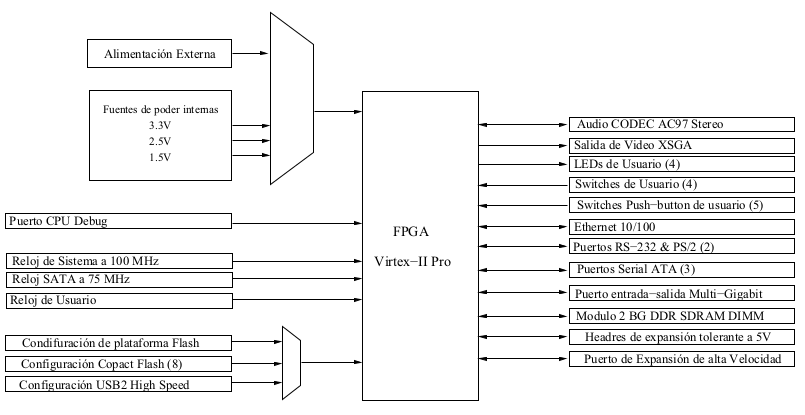
\includegraphics[scale=.50]{./figuras/virtex.png}
 % capas.png: 607x522 pixel, 72dpi, 21.41x18.41 cm, bb=0 0 607 522
 \caption{Diagrama a bloques de la tarjeta Virtex-II Pro 50}
 \label{Diagrama a bloques de la tarjeta Virtex-II Pro 50}
\end{figure}

\begin{verbatim}
#Host x86
#Creacion del directorio de trabajo y descargar buildroot
cd /opt
mkdir toolchains-mips
cd toolchains-mips
wget "http://buildroot.uclibc.org/downloads/buildroot-2011.05.tar.gz"
tar zxvf buildroot-2011.05.tar.gz
cd buildroot-2011.05
\end{verbatim}

Una de las  variables muy importantes para preparar el entorno de compilación, 
es determinar de forma correcta  la arquitectura, por se deben de verificar  
los parametros básicos de la tarejeta de desarrollo :

\begin{verbatim}
[root@XUPV2P-MicheAngelo ~]# cat /proc/cpuinfo                                  
processor       : 0                                                             
cpu             : Virtex-II Pro                                                 
clock           : 300.000000MHz                                                 
revision        : 8.160 (pvr 2001 08a0)                                         
bogomips        : 600.00                                                        
timebase        : 300000000                                                     
platform        : Xilinx Virtex                                                 
model           : testing                                                       
Memory          : 128 MB 
\end{verbatim}

Una vez que \emph{buildroot} genere la toolchain que se usará para la 
compilación de ClamAV se deberán de cambiar las variables de entorno a través 
de la ejecucion del siguiente script:


\lstinputlisting[caption=Archivo variables.sh,language=sh]
{./code/variables.sh}


Una vez  cargadas la variables de entorno de procede a preparar la instalación 
de   clamAV primero se deber\'a configurar el archivo ``.config''
\begin{verbatim}
 Proyecto@debian$./configure --enable-experimental
\end{verbatim}

Tras lo cual se obtiene la siguiente salida:
\begin{verbatim}
checking build system type... x86_64-unknown-linux-gnu
checking host system type... x86_64-unknown-linux-gnu
checking target system type... x86_64-unknown-linux-gnu
creating target.h - canonical system defines
checking for a BSD-compatible install... /usr/bin/install -c
checking whether build environment is sane... yes
checking for a thread-safe mkdir -p... /bin/mkdir -p
checking for gawk... no
checking for mawk... mawk
checking whether make sets $(MAKE)... yes
checking how to create a ustar tar archive... gnutar
checking for gawk... (cached) mawk
checking for a BSD-compatible install... /usr/bin/install -c
checking whether ln -s works... yes
checking whether make sets $(MAKE)... (cached) yes
checking for style of include used by make... GNU
checking for gcc... 
/home/Proyecto/buildroot-2013.05/output/host/usr/bin/powerpc-linux-gcc
checking for C compiler default output file name... a.out
checking whether the C compiler works... configure: error: in 
`/home/henry/buildroot-2013.05/clamav-0.97.8':
configure: error: cannot run C compiled programs.
If you meant to cross compile, use `--host'.
See `config.log' for more details.
\end{verbatim}


Este error en el archivo nos indica que  es necesario utilizar la bandera 
\emph{--host} si se requiere hacer una compilación cruzada.

Se procede nuevamente a  ejecutar el script  de autoconfiguración añadienendo 
la bandera \emph{--host} con la arquitectura objetivo:

\begin{verbatim}
 Proyecto@debian$./configure --host=ppc-unknown-linux-gnu 
--target=ppc-unknown-linux-gnu --enable-llvm CFLAGS="-O0"  --disable-nls 
--disable-libasprintf

\end{verbatim}


Una vez ejecutado el comando anterior se obtiene:

\begin{verbatim}
configure: Summary of detected features follows
              OS          : linux-gnu
              pthreads    : yes (-lpthread)
configure: Summary of miscellaneous  features
              check       : no (auto)
              fanotify    : yes
              fdpassing   : 0
              IPv6        : no
configure: Summary of optional tools
              clamdtop    : -lncurses (auto)
              milter      : yes (disabled)
configure: Summary of engine performance features)
              release mode: yes
              jit         : yes
              mempool     : no
configure: Summary of engine detection features
              autoit_ea06 : yes
              bzip2       : ok
              zlib        : /usr
              unrar       : yes
configure: WARNING:
****** WARNING:
****** You are cross compiling to a different host or you are
****** linking to bugged system libraries or you have manually
****** disabled important configure checks.
****** Please be aware that this build may be badly broken.
****** DO NOT REPORT BUGS BASED ON THIS BUILD !!!


\end{verbatim}

La salida completa del script  de autoconfiguración se muestra en el 
\emph{Apéndice B}.


Antes de continuar con el proceso de compilación es necesario desinstalar 
cualquier  verisión de ClamAV previamente instalada:

\begin{verbatim}
 Proyecto@debian$ sudo make uninstall
\end{verbatim}

Y se procede con la instalación para generar los binarios en la arquitectura 
huesped:

\begin{verbatim}
 Proyecto@debian$ sudo make
 Proyecto@debian$ sudo make install
\end{verbatim}


Debido a que se esta realizando una  compilación cruzada, es necesario depurar 
manualmente algunos de los archivos fuente.

Una vez  compilado los archivos fuente del antivirus ClamAV se debe de copiar 
la salida a los directorios correspondientes de la tarjeta a través de 
\emph{ssh} usando el comando  \emph{scp}.


El  antivirus ppuede ser probado en la tarjeta de desarrollo de la siguiente  
forma:

\begin{verbatim}
Proyecto@debian$ cat eicar.com && clamscan eicar.com 
X5O!P%@AP[4\PZX54(P^)7CC)7}$EICAR-STANDARD-ANTIVIRUS-TEST-FILE!$H+H*
eicar.com: Eicar-Test-Signature FOUND

----------- SCAN SUMMARY -----------
Known viruses: 2337113
Engine version: 0.97.8
Scanned directories: 0
Scanned files: 1
Infected files: 1
Data scanned: 0.00 MB
Data read: 0.00 MB (ratio 0.00:1)
Time: 4.861 sec (0 m 4 s)
\end{verbatim}


El archivo anterior es un archivo DOS que consiste de caracteres ASCII con 
68 bytes de longitud.

\begin{verbatim}
 X5O!P%@AP[4\PZX54(P^)7CC)7}$EICAR-STANDARD-ANTIVIRUS-TEST-FILE!$H+H*
\end{verbatim}


El antivirus  implementado  en la tarjeta deberá de  detectar esta y otras 
amenzas mientras  hace  una revisión programada ocn el comendo \emph{clamscan} 
en el sistema empotrado en la FPGA.














% \include{antispam}
% \include{openssh}



\appendix

%% Cap'itulos incluidos despues del comando \appendix aparecen como ap'endices
%% de la tesis.
\chapter{Instalaciòn Xilinx ISE y Xilinx EDK en Linux}\label{ApexA}



\section{Herramientas}

\begin{itemize}
 \item Linux Debian 6.0, Linux Fedora 17, CentOS 6.3
 \item Xilinx EDK 8.2.02 Build EDK\_Im\_Sp2.4
 \item Tarjeta de desarrollo NetFPGA
 \item Bibliotecas libusb y usb-driver
%  \item minicom
\end{itemize}


\section{Requerimeintos}

\section{Instalación del ISE y EDK}


Se deberá de  montar la imágen para acceder a los archivos. 
Para montar algún dispositivo o imágen se debe contar con privilegios de 
super-usuario:

  \begin{verbatim}	
   root@debian:~# mount -t iso9660 -o loop Xilinx_ISE_DS.iso /media/ 
  \end{verbatim}

La ruta de instalación será:

  \begin{verbatim}	
  #/mnt/setup 
  \end{verbatim}
  
\begin{figure}[ht]
  \begin{center}
 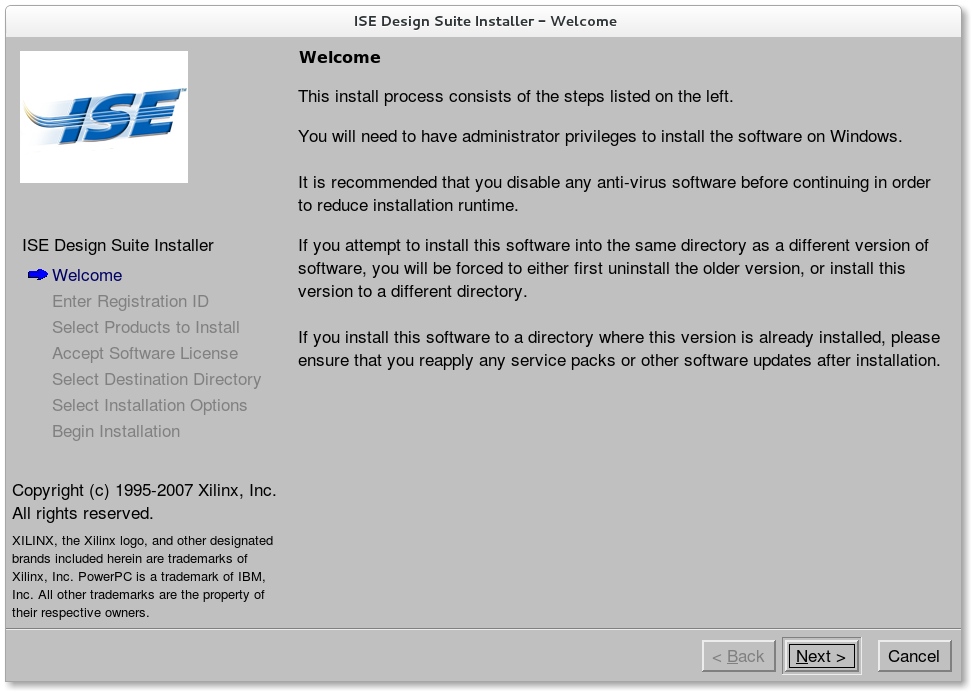
\includegraphics[scale=.40]{./figuras/Installer.png}
  \caption{Pantalla de instalaciòn ISE 8.2}
 \label{Pantalla instalaciòn ISE 8.2}
 % Installer.png: 971x691 pixel, 72dpi, 34.25x24.38 cm, bb=0 0 971 691
 \end{center}
\end{figure}

% Pass: 1472AKH27AD266UHKE980RNMB

En un sistema de escritorio personalizado la instalación creará un directorio
en su \emph{home} llamado Xilinx.

Seleccionamos solo los módulos que necesitamos:
\begin{itemize}
 \item Standalone Programming Tools
 \item ISE Design Tools
 \item Embedded Development Kit (EDK)
 \item ChipScope Pro
 \item PlanAhead Analysis Tool/PlanAhead Lite
\end{itemize}


\begin{figure}[ht]
  \begin{center}
 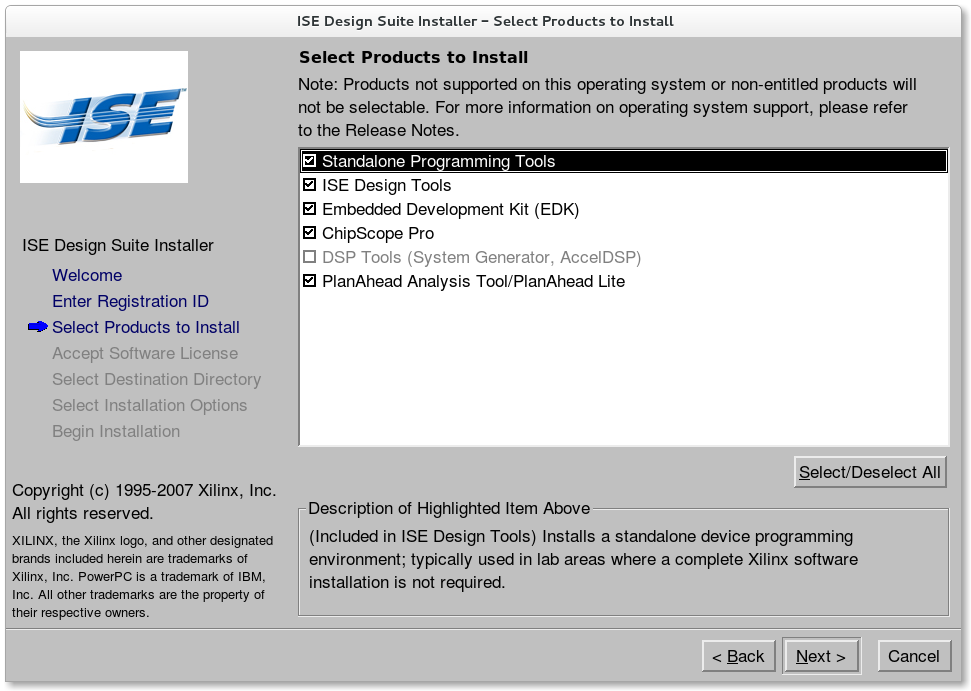
\includegraphics[scale=.40]{./figuras/Modules_install.png}
  \caption{Módulos a instalar}
 \label{Módulos a instalar ISE 8.2}
 % Installer.png: 971x691 pixel, 72dpi, 34.25x24.38 cm, bb=0 0 971 691
 \end{center}
\end{figure}

Se selecciona un directorio para a instalaciòn:

  \begin{verbatim}
  /opt/Xilinx/8.2 
  \end{verbatim}
  
  \begin{figure}[ht]
  \begin{center}
 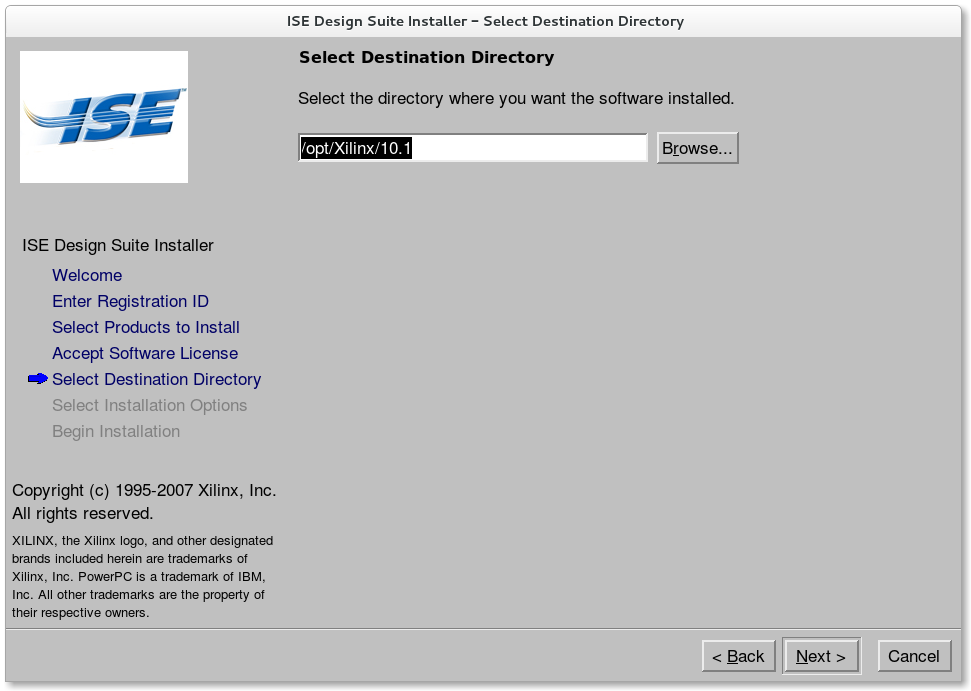
\includegraphics[scale=.40]{./figuras/Directory.png}
  \caption{Directorio de instalaciòn}
 \label{Directorio de instalaciòn ISE 8.2}
 % Installer.png: 971x691 pixel, 72dpi, 34.25x24.38 cm, bb=0 0 971 691
 \end{center}
\end{figure}

\section{Ejecución del ISE y EDK}


Para lanzar tanto ISE como el EDK, será necesario crear variables de ambiente
para la relación de sus aplicaciones, se han creado dos  \emph{scripts} que
facilitan la ejecución, \emph{ise.sh} permite la ejecución de ISE :

\lstinputlisting[caption=Archivo ise.sh,language=sh]{./code/ise.sh}

se agregan permisos de ejecución:

  \begin{verbatim}		
  root@debian:~$chmod +x ise.sh
  \end{verbatim}
 

\emph{edk.sh} permite la ejecución de EDK :

\lstinputlisting[caption=Archivo edk.sh,language=sh]{./code/edk.sh}

se agregan permisos de ejecución:

  \begin{verbatim}	
  Proyecto@debian:~$chmod +x edk.sh
  \end{verbatim}

 se edita el archivo \emph{.bashrc} quedando:
 \lstinputlisting[caption=Archivo .bashrc, language=sh,numbers=none,
]{./code/bashrc}
  
 
  
  se procede a ejecutar ISE :
  
    \begin{verbatim}		
  Proyecto@debian:~$ise
  \end{verbatim}
  
    \begin{figure}[ht]
  \begin{center}
 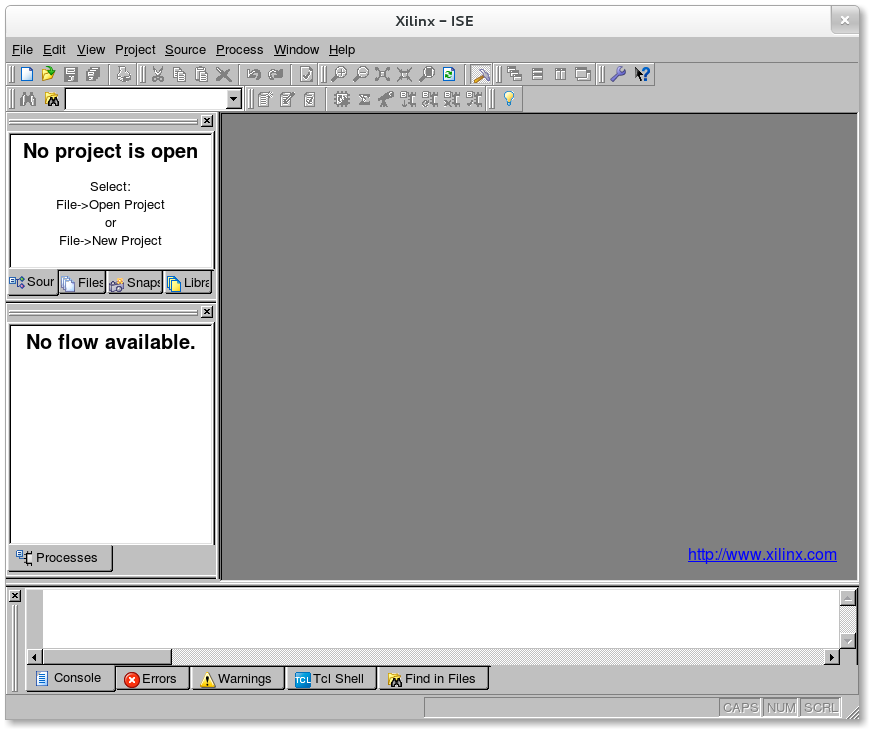
\includegraphics[scale=.40]{./figuras/ise.png}
  \caption{Ejecución de ISE 8.2}
 \label{Ejecución de ISE 8.2}
 % Installer.png: 971x691 pixel, 72dpi, 34.25x24.38 cm, bb=0 0 971 691
 \end{center}
\end{figure}

 por ultimo se ejecuta EDK :
 
     \begin{verbatim}		
  Proyecto@debian:~$edk
  \end{verbatim}
  
    \begin{figure}[ht]
  \begin{center}
 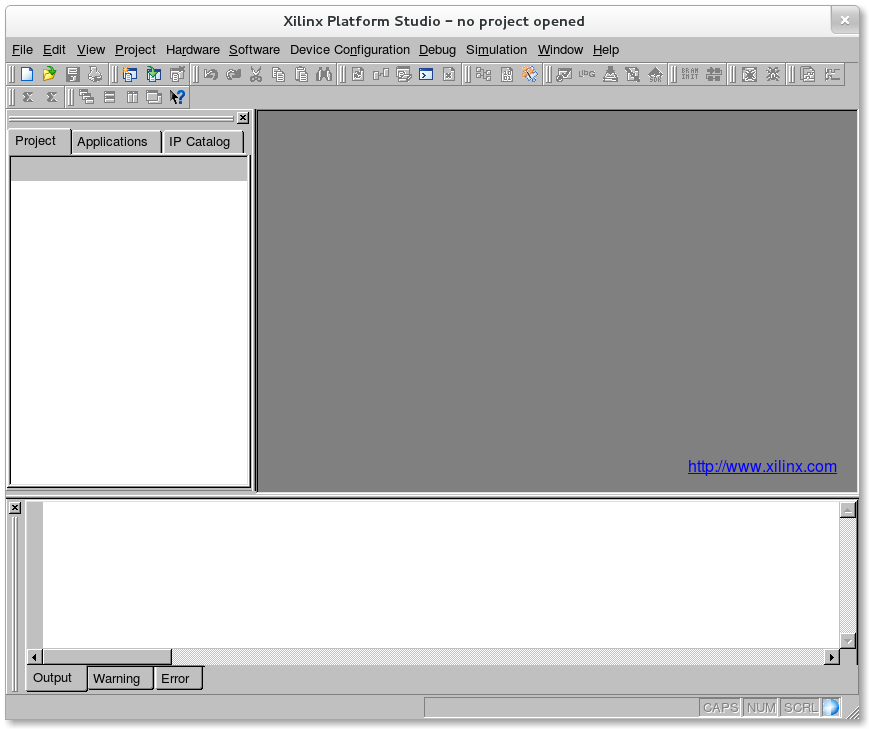
\includegraphics[scale=.40]{./figuras/edk.png}
  \caption{Ejecución de EDK 8.2}
 \label{Ejecución de EDK 8.2}
 % Installer.png: 971x691 pixel, 72dpi, 34.25x24.38 cm, bb=0 0 971 691
 \end{center}
\end{figure}
  
  


 
\chapter{Códigos Fuente}\label{ApexB}

\section{Archivo xilinx.dts}

\lstinputlisting[caption=Archivo xilinx.dts,language=C]{./code/xilinx.dts}

\newpage

\section{Archivo de configuración del \emph{kernel}}

\lstinputlisting[caption=Archivo de configuración del \emph{kernel}
.config,language=C]{./code/config_kernel}

\section{Archivo de configuración \emph{buildroot}}

\lstinputlisting[caption=Archivo de configuración de \emph{Buildroot}
.config,language=C]{./code/config_buildroot}

\section{Arranque del sistema}

\lstinputlisting[caption=Arranque del sistema,language=sh]{./code/xupv2salida}



\section{Script de autoconfiguración \emph{ClamAV}}
\lstinputlisting[caption=Script de AutoConfiguraci\'on 
ClamAV,language=sh]{./code/configure.txt}


\section{Archivo de configuración \emph{ClamAV}}
\lstinputlisting[caption=Configuraci\'on 
ClamAV,language=sh]{./code/freshclam.conf}




%% # Bibliograf'ia#

\bibliography{biblio}

\end{document}
